%\begin{filecontents}
%  @CONTROL{apsrev41Control,title="0"%,author="48",editor="1",pages="1",year="0"}
%\end{filecontents}
\RequirePackage[l2tabu, orthodox]{nag}
\RequirePackage{fixltx2e}
\RequirePackage{fix-cm}
\PassOptionsToPackage{pdftex,psdextra=true,
pdfversion=1.7,
pdfencoding=auto,
pdfnewwindow=true,
pdfusetitle=true,
psdextra=true,
%pdftoolbar=true,
%pdfmenubar=true,
bookmarks=true,
bookmarksnumbered=true,
bookmarksopen=true,
pdfpagemode=UseThumbs,
bookmarksopenlevel=1,
pdfpagelabels=false
}{hyperref}
\PassOptionsToPackage{usenames,dvipsnames}{xcolor}
\documentclass[aps,english,superscriptaddress,onecolumn,twoside,longbibliography,pra,floatfix,fleqn,nofootinbib]{revtex4-1}%


\usepackage[utf8]{inputenx}% for arXiv use encoding ansinew
\input{ix-utf8enc.dfu}
%\usepackage[utf8x]{inputenc}% for arXiv use encoding ansinew
%\usepackage{utf8mathlite}% custom style sheet for unicode-ish math
%\usepackage{newunicodechar}
%\newunicodechar{∫}{\int}
%\usepackage{unicode-math}
\usepackage[OT1]{fontenc}
\usepackage{ucs} %for unichar

\usepackage{amsfonts}
\usepackage{amssymb}
\usepackage{amsthm}
\usepackage[intlimits,fleqn]{amsmath}
%\usepackage{mathdots}
\usepackage{graphicx}%
\usepackage{placeins} %for FloatBarrier
\usepackage{afterpage} %for FloatBarrier in afterpage wrapper
%\usepackage{flushend}
%\usepackage{dblfloatfix}
\usepackage[normalem]{ulem} %for sout
\usepackage[raggedright,bf,nooneline]{subfigure}
\renewcommand{\thesubfigure}{\alph{subfigure}}
\usepackage{paralist}

%\usepackage{ellipsis}
\usepackage{float}% (not with floatrow)
\usepackage{wrapfig}
%\usepackage{floatrow}

\usepackage{marvosym} % for \Smiley and \Frowny
\usepackage{setspace}
\usepackage{array}
\usepackage{ragged2e}%for justifying text in tables
\usepackage{tabularx}
\def\tabularxcolumn#1{m{#1}}
\usepackage{booktabs}
%\usepackage{tabulary}
\newcolumntype{R}{>{\raggedleft\arraybackslash}X}
\newcolumntype{C}{>{\centering\arraybackslash}X}
\newcolumntype{L}{>{\raggedright\arraybackslash}X}
\newcolumntype{J}{>{\justifying\arraybackslash}X}
\usepackage{adjustbox}
\usepackage{multirow}
\newcolumntype{T}[2]{%
    >{\adjustbox{angle=#1,lap=\width-(#2)}\bgroup}%
    l%
    <{\egroup}%
}
\newcommand*\rot{\multicolumn{1}{T{90}{1em}}}% no optional argument here, please!

\setcounter{MaxMatrixCols}{30}
\providecommand{\U}[1]{\protect\rule{.1in}{.1in}}
%EndMSIPreambleData
\newtheorem{theorem}{Theorem}
\newtheorem{acknowledgement}[theorem]{Acknowledgement}
\newtheorem{algorithm}[theorem]{Algorithm}
\newtheorem{axiom}[theorem]{Axiom}
\newtheorem{claim}[theorem]{Claim}
\newtheorem{conclusion}[theorem]{Conclusion}
\newtheorem{condition}[theorem]{Condition}
\newtheorem{conjecture}[theorem]{Conjecture}
\newtheorem{corollary}[theorem]{Corollary}
%\newtheorem{corollary}{Corollary}[theorem] - subindexing, not used here
\newtheorem{criterion}[theorem]{Criterion}
\newtheorem{definition}[theorem]{Definition}
%\newtheorem{example}[theorem]{Example}
\newtheorem{exercise}[theorem]{Exercise}
\newtheorem{lemma}[theorem]{Lemma}
\newtheorem{notation}[theorem]{Notation}
\newtheorem{problem}[theorem]{Problem}
\newtheorem{prop}{Proposition}
\newtheorem{taut}{Tautology}
\newtheorem{remark}[theorem]{Remark}
\newtheorem{solution}[theorem]{Solution}
\newtheorem{summary}[theorem]{Summary}
%\newenvironment{proof}[1][Proof]{\noindent\textbf{#1.} }{\ \rule{0.5em}{0.5em}}

% hyperlink stuff
\usepackage[usenames,dvipsnames]{xcolor}
\definecolor{ultramarine}{RGB}{63, 0, 255}
\definecolor{medblue}{RGB}{0, 0, 100}
\definecolor{panblue}{RGB}{0,24,150}
\definecolor{carmine}{RGB}{150, 0, 24}
\usepackage[breaklinks=true]{hyperref}
\hypersetup{colorlinks,
linkcolor=carmine,
citecolor=medblue,
urlcolor=panblue,
anchorcolor=OliveGreen}
%\usepackage{url}
\usepackage{pdfpages}
\newcounter{includepdfpage}

\definecolor{purple}{RGB}{128,0,128}
\definecolor{PURPLE}{RGB}{128,0,128}
\definecolor{BLACK}{RGB}{0,0,0}
\definecolor{ultramarine}{RGB}{63, 0, 255}
\definecolor{medblue}{RGB}{0, 0, 100}
\definecolor{panblue}{RGB}{0,24,150}
\definecolor{carmine}{RGB}{150, 0, 24}
\definecolor{gray}{RGB}{150, 150, 150}

\newcommand{\purp}[1]{{\color{purple}{#1}\color{black}}}
\newcommand*{\mred}[1]{{\color{RawSienna}{\mathbf{#1}}}}
\newcommand*{\mblue}[1]{{\color{MidnightBlue}{\ensuremath{#1}}}}
\newcommand*{\mpurp}[1]{{\color{Plum}{\mathbf{#1}}}}
\newcommand*{\mgreen}[1]{{\color{OliveGreen}{\mathbf{#1}}}}
\newcommand*{\tred}[1]{{\color{carmine}{\textbf{#1}}}}
\newcommand*{\tblue}[1]{{\color{MidnightBlue}{\textbf{#1}}}}
\newcommand*{\tpurp}[1]{{\color{Plum}{\textbf{#1}}}}
\newcommand*{\tgreen}[1]{{\color{Sepia}{\textbf{#1}}}}

\newcommand{\quoteby}{\raise.17ex\hbox{$\scriptstyle\sim$}}

\usepackage{verbatim} %for comment command
\usepackage{units}% for nicefrac
\usepackage{xfrac}% for sfrac
\newcommand{\half}[1]{\nicefrac{#1}{2}}

%\usepackage{braket} %provide \bra and \Bra and \set and \Set etc...
%\newcommand{\brackets}[1]{\lbrace{#1\rbrace}}
%\newcommand{\brackets}{\Set}



\usepackage{microtype}
%\usepackage{MnSymbol}
%\usepackage{mathabx}

\usepackage[capitalise]{cleveref}
\Crefname{eqs}{Eqs.}{Eqs.}

\creflabelformat{eqs}{(#2#1#3)}
\crefrangelabelformat{equation}{(#3#1#4-#5#2#6)}
%\crefmultiformat{equation}{eqs.~(#2#1#3)}{ and~(#2#1#3)}{, (#2#1#3)}{ and~(#2#1#3)}
\Crefmultiformat{equation}{Eqs.~(#2#1#3}{,#2#1#3)}{,#2#1#3}{,#2#1#3)}
\crefrangelabelformat{eqs}{(#3#1#4-#5#2#6)}
\Crefmultiformat{eqs}{Eqs.~(#2#1#3}{,#2#1#3)}{,#2#1#3}{,#2#1#3)}
\Crefname{prop}{\textbf{Prop}.}{\textbf{Props}.}
\Crefname{taut}{\textbf{Taut}.}{\textbf{Tauts}.}
\Crefname{section}{Sec.}{Secs.}

%\Crefname{ineq}{Ineq.}{Ineqs.}
%\creflabelformat{ineq}{(#2#1#3)}
%\crefrangelabelformat{ineq}{(#3#1#4-#5#2#6)}
%\Crefmultiformat{ineq}{Ineqs.~(#2#1#3}{,#2#1#3)}{,#2#1#3}{,#2#1#3)}

%\Crefname{ineqs}{Ineqs.}{Ineqs.}
%\creflabelformat{ineqs}{(#2#1#3)}
%\crefrangelabelformat{ineqs}{(#3#1#4-#5#2#6)}
%\Crefmultiformat{ineqs}{Ineqs.~(#2#1#3}{,#2#1#3)}{,#2#1#3}{,#2#1#3)}

\newenvironment{topic}[1][]{\par\medskip\noindent\textbf{\rmfamily#1}}{\par\medskip\par}

\newcounter{step}[section]
\newenvironment{step}[1][]{\refstepcounter{step}\par\medskip
   \noindent \textbf{Step~\thestep}\rmfamily#1}{\par\medskip\par}
%\newenvironment{step}[1][Step]{\noindent\textbf{#1.} }{\ \rule{0.5em}{0.5em}}
\Crefname{step}{Step}{Steps}
\creflabelformat{step}{#2#1#3}
\crefrangelabelformat{step}{#3#1#4-#5#2#6}
\Crefmultiformat{step}{Steps.~#2#1#3}{,#2#1#3}{,#2#1#3}{,#2#1#3}
\renewcommand{\thestep}{\arabic{step}}


\newcounter{example}[section]
\newenvironment{example}[1][]{\refstepcounter{example}\par\medskip
   \noindent \textbf{Example~\theexample}\rmfamily#1}{\par\medskip\par}
%\newenvironment{step}[1][Step]{\noindent\textbf{#1.} }{\ \rule{0.5em}{0.5em}}
\Crefname{example}{Example}{Examples}
\creflabelformat{example}{#2#1#3}
\crefrangelabelformat{example}{#3#1#4-#5#2#6}
\Crefmultiformat{example}{Exmpls.~#2#1#3}{,#2#1#3}{,#2#1#3}{,#2#1#3}
\renewcommand{\theexample}{\arabic{example}}


\usepackage[intlimits,fleqn]{mathtools} %for mathclap and prescript and more. Learning to love this package. And DeclarePairDelimeter!
\DeclarePairedDelimiter{\ceil}{\lceil}{\rceil}
\DeclarePairedDelimiter{\floor}{\lfloor}{\rfloor}
\DeclarePairedDelimiter{\parens}{\lparen}{\rparen}
\DeclarePairedDelimiter{\parenths}{\lparen}{\rparen}
\DeclarePairedDelimiter{\abs}{\lvert}{\rvert}
\DeclarePairedDelimiter{\norm}{\lVert}{\rVert}
\DeclarePairedDelimiter{\braces}{\lbrace}{\rbrace}
\DeclarePairedDelimiter{\bracks}{\lbrack}{\rbrack}
\DeclarePairedDelimiter{\expec}{\langle}{\rangle}
\newcommand{\brackets}[1]{\braces*{#1}}

%\usepackage{nath} %automatically pair delimiters. Provides \inline and \displayed. Adjusts \frac and /

%\newcommand{\na}{\ensuremath{\mathring{a}}}
%\newcommand{\nb}{\ensuremath{\mathring{b}}}
%\newcommand{\nc}{\ensuremath{\mathring{c}}}
\newcommand{\na}{\ensuremath{\overline{a}}}
\newcommand{\nb}{\ensuremath{\overline{b}}}
\newcommand{\nc}{\ensuremath{\overline{c}}}

\newcommand{\naf}{\ensuremath{\lnot a}}
\newcommand{\nbf}{\ensuremath{\lnot b}}
\newcommand{\ncf}{\ensuremath{\lnot c}}

\newcommand{\n}[1]{\ensuremath{\overline{#1}}}
\newcommand{\ot}[1]{\ensuremath{\overline{#1}}}
\newcommand{\Nor}[1]{\operatorname{\mathsf{Nor}}\!\bracks*{#1}}

\newcommand{\larray}[1]{\ensuremath{\begin{array}{l}#1\end{array}}}
\newcommand{\lparens}[1]{\ensuremath{\parens*{\larray{#1}}}}
%\newcommand{\NamedFunction}[2]{\operatorname{\mathsf{#1}}\!\bracks*{#2}}
%\newcommand{\NamedFunction}[2]{\operatorname{\mathsf{#1}}\!\bracks*{\larray{#2}}}
\newcommand{\NamedFunction}[2]{\operatorname{\mathsf{#1}}\!\begin{bmatrix*}[l]#2\end{bmatrix*}}
%\newcommand{\SmallNamedFunction}[2]{\operatorname{\mathsf{#1}}\bracks{#2}}
\newcommand{\SmallNamedFunction}[3][]{{\operatorname{\mathsf{#2}}_{#1}}\bracks{#3}}
\newcommand{\nap}{\ensuremath{a'}}
\newcommand{\nbp}{\ensuremath{b'}}
\newcommand{\ncp}{\ensuremath{c'}}
\newcommand{\napp}{\ensuremath{a''}}
\newcommand{\nbpp}{\ensuremath{b''}}
\newcommand{\ncpp}{\ensuremath{c''}}

\newcommand{\p}[2][]{{P_{#1}}\parenths{#2}}
%\newcommand{\pdf}[1]{\operatorname{\mathsf{PDF}}\!\parenths{#1}}
\newcommand{\pdf}[2][]{{P_{#1}}\parenths{#2}}
\newcommand{\pdfp}[2][]{{P_{#1}}^{\prime}\parenths{#2}}
\newcommand{\pfunc}[1]{P_{#1}}
\newcommand{\An}[2][]{{\mathsf{An}_{#1}}\parenths{#2}}
\newcommand{\Pa}[2][]{{\mathsf{Pa}_{#1}}\parenths{#2}}
\newcommand{\Ch}[2][]{{\mathsf{Ch}_{#1}}\parenths{#2}}
\newcommand{\subgraph}[2][]{{\operatorname{\mathsf{SubDAG}}_{#1}}\parenths[\big]{#2}}
\newcommand{\ansubgraph}[2][]{{\operatorname{\mathsf{AnSubDAG}}_{#1}}\parenths[\big]{#2}}
\newcommand{\pasubgraph}[2][]{{\operatorname{\mathsf{PaSubDAG}}_{#1}}\parenths[\big]{#2}}
\newcommand{\nodes}[1]{\SmallNamedFunction{Nodes}{#1}}
\newcommand{\edges}[1]{\SmallNamedFunction{Edges}{#1}}
\newcommand{\namedand}[1]{\SmallNamedFunction{And}{#1}}
\newcommand{\namedor}[1]{\SmallNamedFunction{Or}{#1}}
%\newcommand{\aindep}{\ensuremath{\mathrel{\mathopen{\Lsh}{\scriptstyle\emptyset}\mathclose{\Rsh}}}}
\newcommand{\aindep}{\perp}

%\newcommand{\subsim}[1]{\substack{\textstyle #1\\[-0.3ex]\sim}}
%\newcommand{\subsim}{\utilde}
%\def\subsim#1{\mathord{\vtop{\ialign{##\crcr
%$\hfil\displaystyle{#1}\hfil$\crcr\noalign{\kern1.5pt\nointerlineskip}
%$\hfil\tilde{}\hfil$\crcr\noalign{\kern1.5pt}}}}}
\newcommand{\subsim}[1]{\tilde{#1}}

\newcommand{\cramp}[1]{\ensuremath{\mathord{#1}}}
%\newcommand{\cramp}[1]{\ensuremath{\mathopen{}#1\mathclose{}}} oldway. New way is better.
\newcommand{\eql}{\cramp{=}}
\newcommand{\neql}{\cramp{\neq}}

\usepackage{bm}
\newcommand{\setlambda}{\bm{\lambda}}


%%%% Tobias: to mark my edits and stuff
%\usepackage{showkeys}
\usepackage[draft]{fixme}
\newcommand{\btob}{\color{OliveGreen}}
\newcommand{\etob}{\color{black}}

% vertical spacing in multiline equations
\setlength{\jot}{6pt}



\let\stdsection\section
%\renewcommand\section{\clearpage\stdsection}%every section new page
%\usepackage{titlesec}

\makeatletter
\def\p@subsection{\thesection-}
\makeatother



\def\indep{\perp\!\!\!\!\perp}

\begin{document}

\title{The Inflation Technique for Causal Inference with Latent Variables}

\author{Elie Wolfe}
\email{ewolfe@perimeterinstitute.ca}
\affiliation{Perimeter Institute for Theoretical Physics, Waterloo, Ontario, Canada, N2L 2Y5}

\author{Robert W. Spekkens}
\email{rspekkens@perimeterinstitute.ca}
\affiliation{Perimeter Institute for Theoretical Physics, Waterloo, Ontario, Canada, N2L 2Y5}

\author{Tobias Fritz}
\email{fritz@mis.mpg.de}
\affiliation{Perimeter Institute for Theoretical Physics, Waterloo, Ontario, Canada, N2L 2Y5}
\affiliation{Max Planck Institute for Mathematics in the Sciences, Leipzig, Germany}

\date{\today}


\begin{abstract}

The fundamental problem of causal inference is to determine whether or not a given probability distribution over observed variables is compatible with some causal structure (which may incorporate latent variables).  
It is therefore valuable to be able to derive inequalities whose violation by a distribution witnesses the incompatibility of that distribution with the given causal structure.  We term these causal compatibility inequalities. 
Prominent examples are Bell inequalities and Pearl's instrumental inequality.
% but these each pertain to only a single specific causal structure.  
%Such inequalities arise in many fields.  
%The problem of causal inference via incompatibility witnesses comes up in many fields. Special causal compatibility inequalities are Bell inequalities (which distinguish non-classical from classical distributions) and Tsirelson inequalities (which distinguish quantum from post-quantum distributions), and Pearl's instrumental inequality. All of these are limited to very specific causal structures. 
%Analogues of such inequalities for more-general causal structures, i.e., necessary criteria for either classical or quantum distributions to be realizable from the structure, are highly sought after. 
We here introduce a technique for deriving such inequalities for arbitrary causal structures.
 It consists of blowing up or {\em inflating} the causal structure of interest to a new causal structure that can contain multiple copies of each of the original variables.
%, a process we call {\em inflation}.  
By construction, any causal compatibility inequality on the inflated structure can be translated into one for the original structure. Because inflation often introduces novel $d$-separation relations, it often generates easy opportunities for such translations. 
% {\em obvious} inequalities on the inflated structure which yield nonobvious inequalities for the original structure. 
\begin{comment}
The inflation map is defined in such a way that any causal compatability inequality on the inflated structure can be translated into one for the original structure.  It often introduces novel d-separation relations among the observed variables, which in turn lead to obvious inequalities for the inflated structure that are then translatable into nonobvious inequalities for the original structure. 
\end{comment}
%first \textit{inflating} the causal structure and then translating weak constraints on the inflated structure into stronger constraints on the original structure. 
%We provide several examples of how the technique is powerful enough to rederive known results, such as the Bell inequalities, and 
We demonstrate the technique's power by numerically deriving all of the constraints that it implies for a particular concrete example---an inflation of the so-called triangle scenario
---obtaining a set of causal compatibility inequalities that are provably stronger than those derived from other techniques.
%Concretely, we derive polynomial inequalities for the so-called Triangle scenario, and we show how all Bell inequalities also follow from our method. %analyze Pearl's instrumental inequality from our perspective. 
%We also show that if one is 
Given a {\em specific} probability distribution and a causal structure, our technique provides an efficient means of witnessing their incompatibility.
%can be used to efficiently witness their incompatibility.
%, without requiring explicit inequalities.
\begin{comment}
Furthermore, given both a causal structure and a specific probability distribution, our technique can be used to efficiently witness their incompatibility, without requiring explicit inequalities. The inflation technique is therefore both relevant and practical for general causal inference tasks with latent variables.
\end{comment}
Finally, we discuss how to identify, among the causal compatibility inequalities that the technique yields, those that remain necessary conditions on compatibility even for quantum (and post-quantum) generalizations of the notion of a causal model.
%a quantum generalization of the notion of a causal model as well as for a post-quantum generalization of the notion of a causal model (so-called generalized probabilistic theories).  
%Moreover, we show that our technique can be used to also derive causal compatibility inequalities for causal models that obey quantum theory and for causal models that are neither classical nor quantum but rather obey some generalized probabilistic theories.  
%Moreover, we show how our technique can be tuned to yield either classical witnesses (i.e., that may have quantum violations), or post-classical witnesses (i.e., that hold even in the context of general probability theories), depending on whether or not the inflation implicitly broadcasts the value of a  latent variable. 



\end{abstract}
\maketitle
\tableofcontents

\section{Introduction}

Given a joint probability distribution of some observed variables, the problem of \tblue{causal inference} is to determine which hypotheses about the causal mechanism can explain the given distribution. Here, a causal mechanism may comprise both causal relations among the observed variables, as well as among these and a number of unobserved variables.
%what causal relations could hold among the set of variables that includes these as well as a putative set of unobserved variables that act upon them. 
%, among the observed variables themselves or among these and a putative set of unobserved variables, could  this distribution.
%among these variables and possibly also some unobserved variables could have generated this distribution.
 Causal inference problems arise in a wide variety of scientific disciplines, from sussing out biological pathways to enabling machine learning \cite{pearl2009causality,spirtes2011causation,studeny2005probabilistic,koller2009probabilistic}. A closely related type of problem is to determine, for a given set of causal relations, the set of all distributions of observed variables that can be generated from them.   
A special case of both problems is the following decision problem: given a probability distribution and a hypothesis about the causal relations, determine whether the two are compatible: could the given distribution have been generated by the hypothesized causal relations? This is the problem that we focus on.
%solving the decision problem and for 
We develop necessary conditions for a given distribution to be compatible with a given hypothesis about the causal relations.

%\tblue{infeasibility criteria}, i.e., observable constraints such that the their violation implies the invalidity of the hypothesis as an explanation for observational data. 

In the simplest setting, the causal hypothesis consists of a directed acyclic graph (DAG) {\em all} of whose nodes correspond to observed variables. In this case, obtaining a verdict on the compatibility of a given distribution with the causal hypothesis is simple: the compatibility holds if and only if the distribution is Markov with respect to the DAG, which is to say that the distribution features all of the conditional independence relations asserted by $d$-separation with respect to the DAG. 
%(Recall that variables $X$ and $Y$ are conditionally independent given $Z$ if $P_{X,Y|Z}(xy|z) =P_{X|Z}(x|z) P_{Y|Z}(y|z) \;\forall z: P_{Z}(z)>0.$  We denote this in the conventional way:  $(X\indep Y\text{ }|\text{ }Z)$.) 
The compatible DAGs can be determined algorithmically solely from the distribution~\cite{pearl2009causality}.
%. \sout{ i.e.~without having an \emph{a priori} hypothesis}

A significantly more difficult case is when one considers a causal hypothesis which consists of a DAG whose nodes include \tblue{latent} (i.e., unobserved) variables, so that the set of observed variables is a strict subset of the nodes of the DAG. This case occurs, e.g.,~in situations where one needs to deal with the possible presence of unobserved confounders, and is particularly relevant for experimental design in statistics. 

It is useful to distinguish two varieties of this problem: (i) the causal hypothesis specifies that the latent variables are discrete and of a particular cardinality\footnote{The cardinality of a variable is the number of possible values it can take.}, and (ii) the nature of the latent variables is arbitrary.  

Consider the first variety of causal inference problem, where the cardinalities of the latent variables are all finite. Then the mathematical problem which one must solve to infer the distributions that are compatible with the hypothesis is a quantifier elimination problem for some finite number of quantifiers, as follows. The probabilities making up the distribution over the observed variables can all be expressed as functions of the parameters specifying the conditional probabilities of each node given its parents, many of which involve latent variables. If one can eliminate these unobservable parameters, then one obtains constraints that refer exclusively to the probability distribution over the observed variables.  This is a {\em nonlinear} quantifier elimination problem. While the Tarski-Seidenberg theorem provides an \emph{in principle} algorithm for an exact solution, the computational complexity of such quantifier elimination techniques is too large to be practical, except in particularly simple scenarios~\cite{LeeSpekkens}. Techniques for finding approximate solutions to nonlinear quantifier elimination may help~\cite{ChavesPolynomial}.

The second variety of causal inference problem, where the latent variables are arbitrary, is even more difficult, but also the case that has been the focus of most research and that motivates the present work. It is conceivable that inference problems of this variety can be expressed as quantifier elimination problems as well. This would be the case, for instance, if one could show that latent variables of a certain finite cardinality (as opposed to arbitrary latent variables) are sufficient to generate all the distributions compatible with that DAG\footnote{\citet{rosset2016finite} have an unpublished proof purporting to upper bound the cardinality of sufficiently general latent variables. We do not pursue the question here.}. At present, the problem of finding an algorithm for deciding compatibility in this second case---let alone an efficient algorithm---remains open.  Even if it {\em is} possible to achieve a reduction to the case of latent variables with finite cardinality, one would still be faced with the above nonlinear quantifier elimination problem. As such, heuristic techniques for obtaining nontrivial constraints, such as the one presented in this work, are more important in practice. 

If one allows for latent variables, then the condition that all of the conditional independence relations among the observed variables should be explained by the structure of the DAG is still a necessary condition for compatibility of a DAG with a given distribution, but in general it is no longer a sufficient condition for compatibility. Historically, the insufficiency of the conditional independence relations for causal inference in the presence of latent variables was first noted by Bell in the context of the hidden variable problem in quantum physics~\cite{bell1964einstein}. Bell considered an experiment for which considerations from relativity theory implied a very particular causal structure, and he derived an inequality that any distribution compatible with this structure, and compatible with certain constraints imposed by quantum theory, must satisfy.  Bell also showed that this inequality was violated by distributions generated from entangled quantum states with particular choices of incompatible measurements.
%\footnote{This violation has subsequently become known as \emph{quantum nonlocality}~\cite{Brunner2013Bell}.  
Later work, by Clauser, Horne, Shimony and Holte (CHSH) \cite{CHSHOriginal} showed how to derive inequalities directly from the causal structure. The CHSH inequality was the first example of a compatibility condition that appealed to the strength of the correlations rather than simply the conditional independence relations inherent therein.  Since then, many generalizations of the CHSH inequality have been derived for the same sort of causal structure~\cite{Brunner2013Bell}. The idea that such work is best understood as a contribution to the field of causal inference has only recently been put forward~\cite{WoodSpekkens,fritz2012bell,pusey2014gdag,BeyondBellII}, as has the idea that techniques developed by researchers in the foundations of quantum theory may be usefully adapted to causal inference\footnote{The current article being another example of the phenomenon \cite{ChavesNoSignalling,chaves2014informationinference,weilenmann2016entropic,kela2016covariance,ChavesPolynomial,TavakoliStarNetworks,RossetNetworks,TavakoliNoncyclicNetworks}.}.

Subsequent to Bell's work, Pearl derived an inequality, called the \tblue{instrumental inequality}~\cite{pearl1995instrumental}, which provides a necessary condition for the compatibility of a distribution with a causal structure 
known as the \emph{instrumental scenario} that applies, for instance, to certain kinds of noncompliance in drug trials. \citet{steudel2010ancestors} later derived an inequality which must hold whenever a distribution on $n$
variables is compatible with a causal structure where no set of more
than $c$ variables has a common ancestor, for arbitrary $n,c \in \mathbb{N}$.  Subsequent work has focused specifically on the case of $n=3$ and $c=2$, a causal structure that has been called the Triangle scenario~\cite{fritz2012bell,chaves2014novel}.

Recently, Henson, Lal and Pusey~\cite{pusey2014gdag} have found a sufficient condition for a DAG to be {\em interesting}, by which they mean that conditional independence relations do not exhaust the set  of constraints on the compatibility of a joint distribution over observed variables with the DAG. They also presented a catalogue of all potentially interesting DAGs having six or fewer nodes in~\cite[App.~E]{pusey2014gdag}, of which all but three were shown to be indeed interesting. The Bell scenario, the Instrumental scenario, and the Triangle scenario appear in the catalogue together with many others.   Furthermore, the fraction of DAGs that are interesting increases as the total number of nodes increases.  This highlights the need for moving beyond a case-by-case consideration of individual DAGs and for developing techniques for deriving constraints beyond conditional independence relations that can be applied to any interesting DAG, such as Shannon-type entropic inequalities~\cite{steudel2010ancestors,fritz2012bell,fritz2013marginal,chaves2014novel,chaves2014informationinference}. They can be derived for a given DAG with relative ease, via exclusively linear quantifier elimination, since conditional independence relations are linear equations at the level of entropies. They also have the advantage that they apply regardless of the cardinality of the observable variables. Recent work has also looked at non-Shannon type inequalities, potentially further strengthening the entropic constraints~\cite{weilenmann2016entropic,pianaar2016interesting}. However, entropic techniques are still wanting, since the resulting inequalities are often rather weak. For example, they are not sensitive enough to distinguish uniquely-quantum correlations from their classical causal counterparts~\cite{fritz2012bell,weilenmann2016entropic}\footnote{It should be noted that non-standard entropic inequalities can be obtained through a fine-graining of the causal scenario, namely by \emph{conditioning} on the distinct finite possible outcomes of root variables (``settings''), and these types of inequalities \emph{have} proven somewhat quantum-sensitive \cite{braunstein1988entropic,SchumacherInequality,chaves2014novel}. Such inequalities are still limited, however, in that they are only applicable to those DAGs which feature observable root nodes. The potential utility of entropic analysis where fine-graining is generalized to \emph{non}-root observable nodes is currently being explored by E.W. and Rafael Chaves. Jacques Pienaar has also alluded to similar considerations as a possible avenue for further research~\cite{pianaar2016interesting}.}.

%In contexts other than quantum theory, the latent nodes in causal structures are generally taken to represent hidden variables. This is not fully general, however, so we apply the retronym\footnote{Retronym (noun): a modification of an original term to distinguish it from a later development \cite{retronym}.} ``classical", as in classical causal structure and classical causal inference. The classical distributions of a given causal structure are defined as those which arise from it while restricting the latent nodes to be arbitrary (classical) random variables. Quantum distributions, by contrast, are those which are realizable if the latent nodes in the causal structure are allowed to be quantum systems. We hereafter take all causal structures and probability distributions to be classical, except where explicitly stated otherwise.

%From a physics perspective, therefore, tightly characterizing the set of observable probability distributions realizable from a causal structure is critical, in order to recognize and exploit the existence of distributions that can be realized quantumly but not classically. Few techniques are known for bounding this set of distributions which are simultaneously practical and applicable to general causal structures. Celebrated examples include the use of conditional independence relations (easy) \cite{pearl2009causality,spirtes2011causation,studeny2005probabilistic,koller2009probabilistic} and entropic inequalities (more advanced) \cite{fritz2013marginal,chaves2014novel,chaves2014informationinference}. In the presence of hidden variables, these criteria only rarely provide a tight characterization, and frequently fail to witness the non-classicality of quantum distributions.% Indeed, all the causal scenarios we shall consider here are instances where conventional causal compatibility criteria are found to be insufficient 

%Distinguishing quantum from classical correlations has historically been achieved through the use of Bell inequalities \cite{bell1966lhvm,GisinFramework2012,scarani2012device,Brunner2013Bell,BancalDIApproach}. Bell inequalities, however, are limited to very special causal scenarios involving \emph{only one} latent common cause variable, i.e.~Bell scenarios. A Bell scenario is also very special in that its realizable distributions admit characterization by a finite set of linear inequalities (after conditioning on the setting variables), i.e.~its realizable distributions comprise a convex polytope \cite{GisinFramework2012,FritzDuality}. %The nonconvexity of distributions realizable from a general structure is explicitly evidenced here. 
%Entirely new techniques, therefore, are required to derive quantum-sensitive incompatibility witnesses for more general causal scenarios \cite{fritz2012bell,pusey2014gdag,BeyondBellII}. 

Thus we here introduce a new technique for deriving necessary conditions for the compatibility of a distribution over observed variables with a given causal structure, which we term the {\em inflation technique}. Our technique is frequently capable of witnessing incompatibility when many other causal inference techniques fail. For example, in \cref{example:noWdist} of \cref{subsec:witnessingincompat} we prove that the tripartite ``W-type'' distribution is incompatible with the Triangle scenario, despite the incompatibility being invisible to other causal inference tools such as conditional independence relations, Shannon-type~\cite{fritz2013marginal,chaves2014novel,chaves2014informationinference} or non-Shanon-type entropic inequalities~\cite{weilenmann2016entropic}, or covariance matrices~\cite{kela2016covariance}.


The inflation technique works roughly as follows. For a given DAG under consideration, one can construct many new DAGs, termed {\em inflations} of this DAG. These duplicate one or more of the nodes of the original DAG, while preserving their ancestral subgraph.  Furthermore, the causal parameters that one adds to the inflated DAG are constrained to mirror those of the original DAG.  We show that if the distributions over certain subsets of the observed variables are compatible with the original DAG, then the same distributions over certain copies of those subsets in the inflated DAG are compatible with the inflated DAG.  Similarly, we show that any necessary condition for compatibility of a distribution with the inflated DAG translates into a necessary condition for compatibility with the original DAG.  Thus standard techniques for deriving inequalities, applied to the inflated DAG, can be supplemented with the inflation technique to derive surprisingly strong inequalities for the original DAG.  Concretely, we consider inequalities on the inflated DAG that are obtained from the \emph{mere existence of a joint distribution} on the inflated DAG, supplemented with independence constraints arising from the inflated causal structure.   We show how to derive a complete set of such inequalities by enumerating all facets of the associated \tblue{marginal polytope}. We also show how to compute a partial solution more efficiently by enumerating transversals of a certain hypergraph. Translating these back to the original DAG results in causal compatibility conditions in the form of nonlinear \emph{polynomial inequalities}.
% An inflated DAG naturally carries inflated models, and the existence of an inflated model implies inequalities which constrain the set of distributions on observable nodes compatible with the original causal structure. Polynomial inequalities can be obtained through \emph{linear} inequalities which are necessary conditions for a collection of given marginal distributions to arise from a joint distribution (marginal problem). For deriving such inequalities in turn, we have considered the methods of computing all facets of the marginal polytope via facet enumeration, and deriving looser constraints more efficiently by enumerating hypergraph transversals.

%, in which case we say that the inequalities are \emph{polynomial}. 
Together with the entropic techniques discussed above, our method is the first systematic tool for causal inference with latent variables that goes beyond observable conditional independence relations while not assuming any bounds on the cardinality of each latent variable. While our method can be used to systematically generate necessary conditions for compatibility with a given causal structure, we do not know whether the set of inequalities thus generated are also sufficient.  
%, and we currently have conflicting evidence on this question. On the one hand, our method rederives all Bell-type inequalities (\cref{sec:Bellscenarios}), but on the other hand 


%\color{purple} [R:We still need to say: That here we have only used ancestral independences in the inflated DAG, but that there are prospects for using arbitrary d-separation criteria as well as other features of the inflated model.  
% Finally, we discuss what applications our technique might have for causal models in quantum theory and generalized probabilistic theories.   
% Elie, could you try to write a first draft of this paragraph?  
 %I'm thinking that perhaps we could fold into this discussion a summary of the paper by referring to the appropriate section as we describe what is done in the paper.
% ]\color{black}

% We show how the no-broadcasting theorem governing quantum theory \cite{NoCloningQuantum1996,NoCloningGeneral2006} can be exploited in order to derive specifically quantum-sensitive infeasibility criteria.
While we present our technique primarily as a tool for standard causal inference, we also briefly discuss applications to {\em quantum} causal models and causal models within generalized probabilistic theories~\cite{fritz2012bell,pusey2014gdag,chaves2014informationinference,BeyondBellII}.  In particular, we discuss when our inequalities are also necessary conditions for a distribution over observed variables to be compatible with a given DAG within any generalized probabilistic theory. 

%\color{purple} [R: provide summary of paper] \color{black}

%While we present our technique primarily as a tool for standard causal inference, we also  comment on the extent to which the inequalities we derive are also necessary conditions on the compatibility of a distribution with a DAG for nonclassical generalizations of the notion of a causal model \cite{fritz2012bell,pusey2014gdag,chaves2014informationinference,BeyondBellII}.Some of the inequalities we derive require us to imagine that the value of a hidden variable can be distributed or \emph{broadcast} to many different observed variables.  The no-broadcasting theorem from quantum theory shows that this is not valid in the non-classical case, and from our perspective this is the reason for the existence of quantum violations of Bell inequalities. Moreover, our technique can also be applied in order to derive criteria that must be satisfied by all distributions that can be generated with latent nodes that are states in quantum theory or any other general probabilistic theory, simply by not assuming the possibility of broadcasting. 


%\section{Notation}
\section{Basic definitions of causal models and compatibility}\label{sec:definitions}

A \tblue{causal model} consists of a pair of objects: a \tblue{causal structure} and a set of \tblue{causal parameters}.  We define each in turn, 
%The causal structure specifies a directed acyclic graph (DAG).  Recall that a DAG $G$ 
but first recall the definition of directed acyclic graph (DAG). A DAG $G$ consists of a finite set of nodes $\nodes{G}$ and a set of directed edges $\edges{G}$, where a directed edge is an ordered pair of nodes. Later, each node will carry a random variable and a directed edge between two nodes corresponds to the possibility of a direct causal influence from one variable to the other. In this way, the edges implement causal relations.

Our terminology for the causal relations between the nodes in a DAG is the standard one. The parents of a node $X$ in $G$ are defined as those nodes from which an outgoing edge terminates at $X$, i.e. $\Pa[G]{X} = \{\:Y\:|\:Y\to X\:\}$. When the graph $G$ is clear from the context, then we also omit the subscript. Similarly, the children of a node $X$ in a given graph $G$ are defined as those nodes at which edges originating at $X$ terminate, i.e. $\Ch[G]{X} = \{\:Y\:|\: X\to Y\:\}$. If $\bm{U}$ is a set of nodes, then we put $\Pa[G]{\bm{U}} := \bigcup_{X\in\bm{U}} \Pa[G]{X}$ and $\Ch[G]{\bm{U}} := \bigcup_{X\in\bm{U}} \Ch[G]{X}$. The \tblue{ancestors} of a set of nodes $\bm{U}$, denoted $\An[G]{\bm{U}}$, are defined as those nodes which have a directed \emph{path} to some node in $\bm{U}$, \emph{including the nodes in $\bm{U}$ themselves}\footnote{Note the anti-colloquial self-inclusive definition of ``ancestors" here. We use this definition so that any correlation between two variables can always be attributed to a common ``ancestor'', folding the case whence one variable is e.g.~a parent of the other into the umbrella of common ancestry.}. %{\color{purple} R: Does Pearl include $U$ among the ancestors?  I wonder if ``ancestry'' might be better terminology.} 
Equivalently, $\An{\bm{U}} := \bigcup_{n\in\mathbb{N}} \mathsf{Pa}^n(\bm{U})$, where $\mathsf{Pa}^n(\bm{U})$ is inductively defined via $\mathsf{Pa}^0(\bm{U}) := \bm{U}$ and $\mathsf{Pa}^{n+1}(\bm{U}) := \mathsf{Pa}(\mathsf{Pa}^n(\bm{U}))$. 

A \tblue{causal structure} is a DAG $G$ that incorporates a distinction between two types of nodes: the set of observed nodes $\SmallNamedFunction{ObservedNodes}{G}$, and the set of latent nodes $\SmallNamedFunction{LatentNodes}{G}$.  %Following Ref.~[HensonLalPusey], we will term a DAG that incorporates this distinction a {\em generalized DAG}, or GDAG, and we will denote the observed nodes by triangles and the latent nodes by circles. 
Following~\cite{pusey2014gdag}, we will depict the observed nodes by triangles and the latent nodes by circles, as in~\cref{fig:TriMainDAG}.
%~\footnote{Unlike Ref.~[HensonLalPusey], who term these {\em generalized DAGs}, we will continue to refer to them as simply DAGs. }  
Henceforth, we will use the terms ``DAG'' and ``causal structure'' interchangeably, so that the specification of which variables are observed is considered to be part of the DAG.
% , unless explicitly stated otherwise.
We denote the variable living at a node $X\in\nodes{G}$ by the same letter $X$. Frequently we supplement the causal structure by a specification of the cardinalities of the observable variables at each node.
%Henceforth, we will assume that $G$ denotes not just a DAG, but also the information about which variables are observed and their cardinalities.
%whether it is continuous or discrete, and, if the latter, the cardinality of the set of possible values that the variable can take.

Moving towards causal models, we consider \tblue{causal parameters}. The set of causal parameters specifies, for each node $X$, the conditional probability distribution over the values of the random variable $X$, given the values of the variables $\Pa{X}$.  In the case of root nodes, we have $\Pa{X} = \emptyset$, and the conditional distribution is a plain distribution.
We write $\pfunc{Y|X}$ for the conditional distribution of a variable $Y$ given a variable $X$, while the particular conditional probability of the variable $X$ taking the value $x$ given that the variable $Y$ takes the values $y$ is denoted\footnote{Although our notation suggests that all variables are discrete, we do not make this assumption: all our equations are straightforward to write down in proper measure-theoretical notation.} $\pdf[Y|X]{y|x}$.    Therefore, a given set of causal parameters has the form
\begin{align}
 \{ \pfunc{A|\Pa[G]{A}} : A \in \SmallNamedFunction{Nodes}{G} \}.
\end{align}
%Therefore, a given set of causal parameters, denoted $F_G$, has the form
%\begin{align}
%F_G \equiv \{ \pfunc{A|\Pa[G]{A}} : A \in \SmallNamedFunction{Nodes}{G} \}.
%\end{align}
Finally, a \tblue{causal model} $M$ consists of a causal structure together with a set of causal parameters,
\[
	M = ( G,   \{ \pfunc{A|\Pa[G]{A}} : A \in \SmallNamedFunction{Nodes}{G} \}).
\]
A causal model specifies a joint distribution over all variables in the DAG via
\begin{align}\label{Markov}
P_{\nodes{G}} = \prod_{A\in \SmallNamedFunction{Nodes}{G}} \pfunc{A|\Pa[G]{A}},
\end{align}
where $\prod$ denotes the usual product of functions, so that $(P_X \times P_Y)(x,y) := P_X(x) P_Y(y)$. A distribution $P_{\nodes{G}}$ arises in this way if and only if it satisfies the Markov conditions associated to $G$.
%The subset of nodes of $G$ that are observed is denoted $\SmallNamedFunction{ObservedNodes}{G}$ and the rest are denoted $\SmallNamedFunction{LatentNodes}{G}$. 

The joint distribution over the observed variables is obtained from the joint distribution over all variables by marginalization over the latent variables 
\begin{align}\label{MarkovObserved}
P_{\SmallNamedFunction{ObservedNodes}{G}} =  \sum_{\{X :X \in\SmallNamedFunction{LatentNodes}{G}\}} P_{\SmallNamedFunction{Nodes}{G}},
\end{align}
where $\sum_X$ denotes marginalization over the variable $X$, so that $(\sum_X P_{XY})(y):= \sum_x P_{XY}(xy)$.
%if $P_Y:=\sum_X P_{XY}$, then $P_Y(y) = \sum_x P_{XY}(xy)$.

\begin{comment}
In addition to the notion of a causal model, it is useful to have a notion of a \tblue{causal hypothesis}, which we define to be a set of causal models.  
The most simple sort of causal hypothesis is one that includes the full set of causal models associated to a DAG $G$.  This is simply the hypothesis of a particular DAG, with no restriction on the set of parameters that supplements it.   Examples of more refined hypotheses are provided in Appendix~\ref{App:hypotheses}.
\end{comment}

A given distribution of observed variables is said to be \tblue{compatible} with a given causal structure if there is some choice of the causal parameters that yields the given distribution via Eqs.~\eqref{Markov} and \eqref{MarkovObserved}. Furthermore, a given set of marginal distributions of various subsets of observed variables is said to be compatible with a given causal structure if and only if there exists a joint distribution of observed variables that yields these marginals and is compatible with the causal structure.


%\section{Inflation: a tool for causal inference}
%\section{Witnessing incompatibility using the Inflation technique}
\section{The inflation technique for causal inference}

\subsection{Inflations of a causal model}

We now introduce the notion of \tblue{an inflation of a causal model}.  %Let $C_G$ denote a causal model associated to a DAG $G$.  
If a causal model lives on a DAG $G$, then an inflation of this model lives on an \tblue{inflation DAG} $G'$.  
%An inflation of this model is another causal model, denoted $C_{G'}$ and associated to a different DAG, $G'$.  
There are many possible choices of inflation DAGs $G'$ for a given $G$, forming a set $\SmallNamedFunction{Inflations}{G}$. The choice of $G'\in \SmallNamedFunction{Inflations}{G}$ is the only freedom in the inflation of a causal model.  Once a choice is made, the set of parameters of the inflated model $M'$ is fixed uniquely by the set of parameters of the original model $M$ by a function $M' = \SmallNamedFunction[G\to G']{Inflation}{M}$ that we define below. We begin by defining the condition under which a DAG $G'$  is an inflation of a DAG $G$.  This requires some preliminary definitions. 

The \tblue{induced subgraph} of $G$ obtained by restricting to a subset of nodes $\bm{V}\subseteq \SmallNamedFunction{Nodes}{G}$ will be denoted $\subgraph[G]{\bm{V}}$.
It consists of the nodes $\bm{V}$ and those edges of $G$ of which both endpoints are in $\bm{V}$. Of special importance to us is the 
\tblue{ancestral subgraph} of $\bm{V}$, denoted $\ansubgraph[G]{\bm{V}}$, which is the subgraph induced by the ancestry of $\bm{V}$, $\ansubgraph[G]{\bm{V}}\coloneqq\subgraph[G]{\An[G]{\bm{V}}}$. 

In an inflation DAG $G'$, every node behaves like a copy of a node of $G$. More precisely, the structure of being an inflation DAG also comprises a map $G'\to G$. We call the preimages of a node $A\in\nodes{G}$ the \emph{copies} of $A$ in $G'$, and denote them by $A_1,\ldots, A_k$. The subscript that indexes the copies is termed the \tblue{copy-index}.  When two objects (e.g.~nodes, sets of nodes, DAGs, etc\ldots) are the same up to copy-indices, then we use $\sim$ to indicate this, as in $A_i\sim A_j\sim A$. Other examples are that $\bm{U}\sim\bm{U'}$ for sets of nodes $\bm{U}\subseteq\nodes{G}$ and $\bm{U}'\subseteq\nodes{G'}$ if and only if $\bm{U'}$ contains exactly one copy of every node in $\bm{U}$, and similarly $\subgraph[G']{\bm{U}'}\sim\subgraph[G]{\bm{U}}$ means in addition that an edge is present between two nodes in $\bm{U}'$ if and only if it is present between the two associated nodes in $\bm{U}$.

In order to be an inflation, $G'$ must locally mirror the causal structure of $G$:
%, and a set of variables in $G'$ that differ only by copy-index are called a {\em copy set}.  
\begin{definition}
%The necessary condition on $G'$ for being an inflation of $G$ is that
The DAG $G'$ is said to be an \tblue{inflation} of the DAG $G$, that is, $G' \in \SmallNamedFunction{Inflations}{G}$, if and only if  for every node $A_i$ in $G'$, the ancestral subgraph of $A_i$ in $G'$ is equivalent, under removal of the copy-index, to the ancestral subgraph of $A$ in $G$,
\begin{align}\label{eq:definflationDAG}
G' \in\SmallNamedFunction{Inflations}{G} \quad\text{ iff }\quad \forall A_i\in \SmallNamedFunction{Nodes}{G'}:\; \ansubgraph[G']{A_i}\sim\ansubgraph[G]{A}.
\end{align}
\end{definition}
%Given this notational convention, we can formalize the condition for $G'$ to be an inflation of $G$ as follows:

To illustrate the notion of inflation, we consider the DAG of \cref{fig:TriMainDAG}, which is called the {\em Triangle scenario} (for obvious reasons) and which has been studied by many authors [\citealp{pusey2014gdag}~(Fig.~E\#8), \citealp{WoodSpekkens}~(Fig.~18b), \citealp{fritz2012bell}~(Fig.~3), \citealp{chaves2014novel}~(Fig.~6a), \citealp{Chaves2015infoquantum}~(Fig.~1a), \citealp{BilocalCorrelations}~(Fig.~8), \citealp{steudel2010ancestors}~(Fig.~1b), \citealp{chaves2014informationinference}~(Fig.~4b)].
%As an example, consider the Triangle scenario [\citealp{pusey2014gdag}~(Fig.~E\#8), \citealp{WoodSpekkens}~(Fig.~18b), \citealp{fritz2012bell}~(Fig.~3), \citealp{chaves2014novel}~(Fig.~6a), \citealp{Chaves2015infoquantum}~(Fig.~1a), \citealp{BilocalCorrelations}~(Fig.~8), \citealp{steudel2010ancestors}~(Fig.~1b), \citealp{chaves2014informationinference}~(Fig.~4b)]. The associated DAG, the shape of which explains the name, is depicted here in \cref{fig:TriMainDAG}. 
%The Triangle scenario is a correlation scenario in the sense of \citet{fritz2012bell}; see especially Sec. 2.3 there. 
Different inflations of the Triangle scenario are depicted in \cref{fig:TriFullDouble,fig:Tri222,fig:simpleinflation,fig:simplestinflation,fig:TriDagSubA2B1C1}.

\begin{figure}[h]
\centering
\begin{minipage}[t]{0.23\linewidth}
\centering
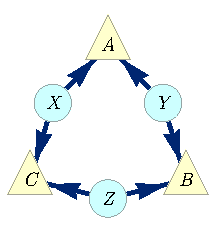
\includegraphics[scale=1]{TriDagRawALT.pdf}
\caption{The causal structure of the Triangle scenario.}\label{fig:TriMainDAG}
\end{minipage}
\hfill
\begin{minipage}[t]{0.43\linewidth}
\centering
\resizebox{\textwidth}{!}{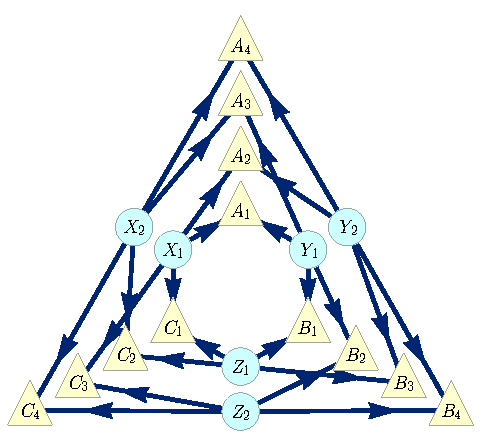
\includegraphics[scale=1]{TriDagFull222ALT.pdf}}
\caption{An inflated DAG of the Triangle scenario where each latent node has been duplicated and each observable nodes node has been quadrupled. The four copies of each observable node correspond to the four possible choices of parentage in the inflated DAG.}\label{fig:TriFullDouble}
\end{minipage}
\hfill
\begin{minipage}[t]{0.3\linewidth}
\centering
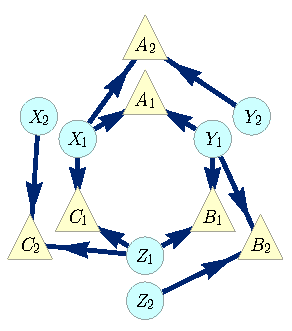
\includegraphics[scale=1]{TriDagSub222fixedcoordALT.pdf}
\caption{Another inflation of the Triangle scenario, also notably $\ansubgraph[(\textrm{\cref{fig:TriFullDouble}})]{A_1 A_2 B_1 B_2 C_1 C_2}$.}\label{fig:Tri222}
\end{minipage}
\end{figure}

\begin{figure}[hb]
\centering
\begin{minipage}[t]{0.3\linewidth}
\centering
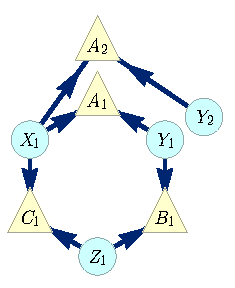
\includegraphics[scale=1]{broadcastingexamplenohighlightALT.pdf}
\caption{A rather simple inflation of the Triangle scenario, also notably $\ansubgraph[(\cref{fig:Tri222})]{A_1 A_2 B_1 C_1}$.}\label{fig:simpleinflation}
\end{minipage}\hfill
\begin{minipage}[t]{0.275\linewidth}
\centering
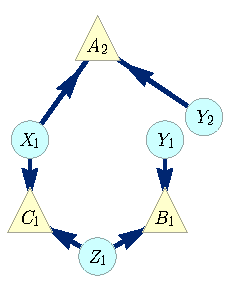
\includegraphics[scale=1]{nobroadcastingexamplenohighlightALT.pdf}
\caption{An even simpler inflation of the Triangle scenario, also notably $\ansubgraph[(\cref{fig:simpleinflation})]{A_2 B_1 C_1}$. }\label{fig:simplestinflation}
\end{minipage}
\hfill
\begin{minipage}[t]{0.325\linewidth}
\centering
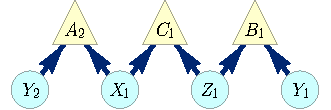
\includegraphics[scale=1]{TriDagSubA2B1C1.pdf}
\caption{A different drawing of \cref{fig:simplestinflation}. Despite not containing the original scenario, this is a valid inflation per~\cref{eq:definflationDAG}.}\label{fig:TriDagSubA2B1C1}
\end{minipage}
\end{figure}

We now define the function $\mathsf{Inflation}_{G\to G'}$, that is, we specify how a causal model inflates.

\begin{definition}
\label[definition]{def:inflat}
Consider causal models $M$ and $M'$ where $\SmallNamedFunction{DAG}{M}=G$ and $\SmallNamedFunction{DAG}{M'}=G'$ and such that $G'$ is an inflation of $G$.   The causal model $M'$ is said to be the {\em \tblue{$G\to G'$ inflation of $M$}}, that is, $M' = \SmallNamedFunction[G\to G']{Inflation}{M}$,  if and only if for every node $A_i$ in $G'$, the manner in which $A_i$ depends causally on its parents within $G'$ is the same as the manner in which $A$ depends causally on its parents within $G$.  Noting that $A_i \sim A$ and that $\Pa[G']{A_i} \sim \Pa[G]{A}$ by~\cref{eq:definflationDAG}, one can formalize this condition as:
\begin{align}\label{eq:funcdependences}
%M' = \SmallNamedFunction{Inflation}{M}_{G\to G'}  \quad \text{iff}\quad 
 \forall A_i \in \SmallNamedFunction{Nodes}{G'}:\; \pfunc{A_i| \Pa[G']{A_i}}=\pfunc{A|\Pa[G]{A}}.
\end{align}
%where Eq.~\eqref{eq:definflationDAG} guarantees that $A_i \sim A$ and $\Pa[G']{A_i} \sim \Pa[G]{A}$.  
\end{definition}

It is clear that for given $G$, $G'$ and $M$, this specifies a unique inflation model $M'$, resulting in a well-defined function ${\operatorname{\mathsf{Inflation}}_{G\to G'}}$. %$\SmallNamedFunction[G\to G']{Inflation}{-}$.

%A causal model specifies the causal structure and the autonomous causal mechanisms.  
To sum up then, the inflation of a causal model is a new causal model where (i) each variable in the original DAG may have counterparts in the inflated DAG with ancestral subgraphs mirroring those of the originals, and (ii) the manner in which a variable depends causally on its parents in the inflated DAG is given by the manner in which its counterpart in the original DAG depends causally on its parents. The operation of modifying a DAG and equipping the modified version with conditional probability distributions that mirror those of the original also appears in the \emph{do calculus} and \emph{twin networks} of~\citet{pearl2009causality}, and moreover bears some resemblance to the \emph{adhesivity} technique used in deriving non-Shannon-type entropic inequalities (App.~\ref{sec:NonShannon}).

We are now in a position to describe the key property of the inflation of a causal model, the one that makes it useful for causal inference. With notation as in \cref{def:inflat}, let %$P$ and $P'$ be the joint distributions over observed variables arising in a causal model $M$ and its inflation $M'$, respectively.  Finally, let
$P_{\bm{U}}$ and $P_{\bm{U}'}$ denote marginal distributions on some sets of nodes $\bm{U}\subseteq\nodes{G}$ and $\bm{U}'\subseteq\nodes{G'}$, respectively. Then
\begin{align}\label{eq:coincidingdistrodef}
%P'_{\bm{U}'}=P_{\bm{U}} 
\quad\text{if }\quad \bm{U}'\sim \bm{U} \;\;\text{and}\;\; \ansubgraph[G']{\bm{U}'}\sim\ansubgraph[G]{\bm{U}}, \quad\text{then}\quad P_{\bm{U}'}=P_{\bm{U}}.
\end{align}
This follows from the fact that the probability distributions over $\bm{U}'$ and $\bm{U}$ depend only on their ancestral subgraphs and the parameters defined thereon, which by the definition of inflation are the same for $\bm{U}'$ and for $\bm{U}$.
It is useful to have a name for those sets of observed nodes in $G'$ which satisfy the antecedent of~\cref{eq:coincidingdistrodef}, that is, for which one can find a copy-index-equivalent set in the original DAG $G$ with a copy-index-equivalent ancestral subgraph.  We call such subsets of the observed nodes of $G'$ \tblue{injectable sets},
\begin{align}\begin{split}\label{eq:definjectable}
&\bm{U}'\in\SmallNamedFunction{InjectableSets}{G'} \\
&\quad\text{ iff }\quad \exists \bm{U}\subseteq \SmallNamedFunction{ObservedNodes}{G} \;\; :\;\; \bm{U}'\sim\bm{U} \;\;\text{and}\;\; \ansubgraph[G']{\bm{U}'}\sim\ansubgraph[G]{\bm{U}}.
\end{split}\end{align}

Similarly,  those sets of observed nodes in the original DAG $G$ which satisfy the antecedent of~\cref{eq:coincidingdistrodef}, that is, for which one can find a corresponding set in the inflated DAG $G'$ with a copy-index-equivalent ancestral subgraph, we describe as \tblue{images of the injectable sets},
\begin{align}\begin{split}\label{eq:defimageinjectable}
& \bm{U}\in\SmallNamedFunction{ImagesInjectableSets}{G} \\
& \quad\text{ iff }\quad \exists \bm{U}' \subseteq \SmallNamedFunction{ObservedNodes}{G'} \;\; :\;\; \bm{U'}\sim\bm{U} \;\;\text{and}\;\; \ansubgraph[G']{\bm{U}'}\sim\ansubgraph[G]{\bm{U}}.
\end{split}\end{align}
Clearly, $\bm{U}\in\SmallNamedFunction{ImagesInjectableSets}{G}$ iff $\exists \bm{U}' \subseteq \SmallNamedFunction{InjectableSets}{G'}$ such that $\bm{U}\sim \bm{U}'$.


For example in the inflation of the Triangle scenario depicted in~\cref{fig:Tri222}, the set of observed nodes $\brackets{A_1 B_1 C_1}$ is injectable because its ancestral subgraph is equivalent up to copy-indices to the ancestral subgraph of $\brackets{A B C}$ in the original DAG, and the set $\brackets{A_2 C_1}$ is injectable because its ancestral subgraph is equivalent to that of $\brackets{ A C}$ in the original DAG. A set of nodes in the inflated DAG can only be injectable if it contains at most one copy of any node from the original DAG. More strongly, it can only be injectable if its ancestral subgraph contains at most one copy of any node from the original DAG.  

Thus, in \cref{fig:Tri222}, $\brackets{A_1 A_2 C_1}$ is not injectable because it contains two copies of $A$, and $\brackets{A_2 B_1 C_1}$ is not injectable because its ancestral subgraph contains two copies of $Y$. The fact that the sets $\brackets{A_1 B_1 C_1}$ and $\brackets{A_2 C_1}$ are injectable implies, via~\cref{eq:coincidingdistrodef}, that the marginals on each of these in the inflation model are precisely equal to the marginals on their counterparts, $\brackets{A B C}$ and $\brackets{A C}$, in the original causal model, so that $P_{A_1 B_1 C_1} = P_{A B C}$ and $P_{A_2 C_1} = P_{A C}$.

It is useful to express \cref{eq:coincidingdistrodef} in the language of injectable sets,
\begin{align}\label{keyinference}
%\text{if }  \quad  \bm{U}'\in\SmallNamedFunction{InjectableSets}{G'} \quad \text{and} \quad \bm{U} \sim \bm{U}'  \quad\text{then}\quad P'_{\bm{U}'}=P_{\bm{U}}.
P_{\bm{U}'}=P_{\bm{U}}\quad\text{if }  \;\; \bm{U}' \sim \bm{U}\;\; \text{and} \;\; \bm{U}'\in\SmallNamedFunction{InjectableSets}{G'}.% \quad \text{and} \quad \bm{U} \sim \bm{U}'  \quad\text{then}\quad P'_{\bm{U}'}=P_{\bm{U}}.
\end{align}

\subsection{Witnessing incompatibility\label{subsec:witnessingincompat}}

Finally, we can explain why inflation is relevant for deciding whether a distribution is compatible with a causal structure.  For a family of marginal distributions $\{ P_{\bm{U}} : \bm{U} \in \SmallNamedFunction{ImagesInjectableSets}{G}\}$ to be compatible with $G$, there must be a causal model $M$ that yields a joint distribution with this family as its marginals. Looking at the inflation model $M' = \SmallNamedFunction[G\to G']{Inflation}{M}$, \cref{keyinference} implies that $M'$ has the corresponding family of marginals given by $\{ P_{\bm{U}'} : \bm{U}' \in \SmallNamedFunction{InjectableSets}{G'}\}$ with $P_{\bm{U}'} = P_{\bm{U}}$ for $\bm{U}'\sim\bm{U}$, and thus this family is compatible with $G'$.

The same considerations apply for subcollections of injectable sets:

\begin{lemma} \label[lemma]{mainlemma}
Let $G'$ an inflation DAG of $G$. 
Let $S'  \subseteq \SmallNamedFunction{InjectableSets}{G'}$ be a collection of injectable sets, and let $S \subseteq \SmallNamedFunction{ImagesInjectableSets}{G}$ be the images of this collection.   If the family of marginal distributions $\{ P_{\bm{U}} : \bm{U} \in S \}$ is compatible with $G$, then the corresponding family of marginal distributions $\{ P_{\bm{U}'} : \bm{U}' \in S' \}$ --- defined via $P           _{\bm{U}'}= P_{\bm{U}}$ for $\bm{U}' \sim \bm{U}$ --- is compatible with $G'$.
\end{lemma}

We have thereby related a question about compatibility with the original causal structure to one about compatibility with the inflated causal structure.  If one can show that the new compatibility question on $G'$ is answered in the negative, then one can infer that the original question is answered in the negative as well.    Some simple examples serve to illustrate the idea.




%\color{purple}
%[Define notational convention of $[x]$]
%\color{black}

\example{: \tred{Witnessing the incompatibility of perfect three-way correlation with the Triangle scenario.}\label{example:noGHZ}}\par\smallskip\nobreak
\begin{figure}[bh]
\centering
\begin{minipage}[t]{0.45\linewidth}
\centering
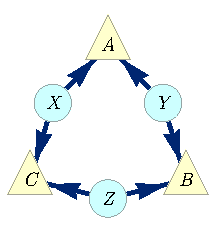
\includegraphics[scale=1]{TriDagRawALT.pdf}
\caption{The causal structure of the Triangle scenario. (Repeat of \cref{fig:TriMainDAG}.)}\label{fig:TriMainDAGv2}
\end{minipage}
\hfill
\begin{minipage}[t]{0.45\linewidth}
\centering
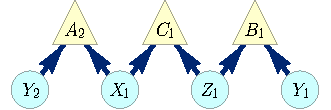
\includegraphics[scale=1]{TriDagSubA2B1C1.pdf}
\caption{A relevant inflation of the Triangle scenario. (Repeat of \cref{fig:TriDagSubA2B1C1}.)}\label{fig:TriDagSubA2B1C1v2}
\end{minipage}
\end{figure}


Consider the following causal inference problem.  One is given a joint distribution over three binary variables, $P_{A B C}$, where the marginal on each variable is uniform and the three are perfectly correlated,
\begin{align}\label{eq:ghzdistribution1}
P_{A B C} =\frac{[000]+[111]}{2},\quad\text{i.e.,}\quad P_{A B C}(a b c)=\begin{cases}\tfrac{1}{2}&\text{if }\; a\eql b\eql c, \\ 0&\text{otherwise},\end{cases}
\end{align}
and one would like to determine whether it is compatible with the Triangle scenario, that is, the DAG depicted in \cref{fig:TriMainDAGv2}.  The sum-over-brackets notation in \cref{eq:ghzdistribution1} is a shorthand for indicating discrete probability distributions: the coefficient of each bracketed tuple indicates the probability of that particular joint outcome.

Since there are no conditional independence relations among the observed variables in the Triangle scenario, there is no opportunity for ruling out the distribution on the grounds that it fails to satisfy the required conditional independences. 

%The causal hypothesis is that the DAG corresponds to the triangle scenario, depicted in \cref{fig:Tri222}.  
%The problem is to decide whether the given distribution is compatible with this causal hypothesis.

To solve this problem, we consider the inflation of the Triangle scenario to the DAG depicted in~\cref{fig:TriDagSubA2B1C1v2}.  
The injectable sets in this case include $\brackets{A_2 C_1}$ and $\brackets{B_1 C_1}$.  We therefore consider the marginals on these sets.

Clearly, the given distribution can only be compatible with the Triangle hypothesis if the following pair of marginals of the given distribution are compatible with the Triangle hypothesis:
\begin{align*}
%\label[eqs]{eq:GHZobsinf}
P_{A C} = P_{B C} = \frac{[00]+[11]}{2}.
\end{align*}
But by \cref{mainlemma}, this compatibility holds only if the following pair of marginals is compatible with the inflation of~\cref{fig:TriDagSubA2B1C1v2},
\begin{align*}
P_{A_2 C_1} = P_{B_1 C_1} = \frac{[00]+[11]}{2}.
\end{align*}

It is not difficult to see that the latter pair of marginals is \emph{not} compatible with our inflated DAG. It suffices to note that the only joint distribution that exhibits perfect correlation between $A_2$ and $C_1$ and between $B_1$ and $C_1$ also exhibits perfect correlation between $A_2$ and $B_1$.  But $A_2$ and $B_1$ have no common ancestors and hence must be marginally independent in the inflated DAG.

We have therefore certified that the joint distribution $P_{A B C}$ of~\cref{eq:ghzdistribution1} is not compatible with the Triangle causal structure, recovering a result originally proven by \citet{steudel2010ancestors}.

\begin{comment}
Let us ask, is it possible for the three original-scenario observable variables $\{A,B,C\}$ to be random but perfectly correlated? We call this the GHZ-type distribution, after an eponymous tripartite entangled quantum state \cite{greenberger1989going,3Qubits2Ways}. So $P_{\text{GHZ}}\parenths{A B C}$ is given by
\begin{align}\label{eq:ghzdistribution1}
p_{\text{GHZ}}\parens{a b c}=\frac{[000]+[111]}{2}=\begin{cases}\tfrac{1}{2}&\text{if }\; a=b=c, \\ 0&\text{otherwise}.\end{cases}
\end{align}
We assume uniform binary variables for the sake of concreteness, but the argument is general. Let's temporarily (falsely) assume $P_{\text{GHZ}}$ to be compatible with the Triangle scenario. Since $\brackets{A_2 C_1}$ is an injectable set we have $\pdf{A_2 C_1}=\pdf{A C}$, and therefore $P_{\text{GHZ}}$ implies that $A_2$ and $C_1$ are perfectly correlated. Similarly, since $\brackets{B_1 C_1}$ is an injectable set we have $\pdf{B_1 C_1}=\pdf{A C}$, and therefore $B_1$ and $C_1$ must be perfectly correlated, and by extension $B_1$ and $A_2$ are perfectly correlated as well. On the other hand, $A_2$ and $B_1$ must be statistically independent, as they do not share any common ancestor. The only way for two variables to be \emph{both} perfectly correlated and independent is by being deterministic. This is not the case in $P_{\text{GHZ}}$, and thus we have certified that $P_{\text{GHZ}}$ is not realizable from the Triangle causal structure, recovering the seminal result of \citet{steudel2010ancestors}.
\end{comment}

\example{: \tred{Witnessing the incompatibility of the W-type distribution with the Triangle scenario}\label{example:noWdist}}\par\smallskip\nobreak
\begin{figure}[bh]
\centering
\begin{minipage}[t]{0.45\linewidth}
\centering
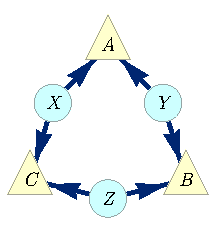
\includegraphics[scale=1]{TriDagRawALT.pdf}
\caption{The causal structure of the Triangle scenario. (Repeat of \cref{fig:TriMainDAG}.)}\label{fig:TriMainDAGv3}
\end{minipage}
\hfill
\begin{minipage}[t]{0.45\linewidth}
\centering
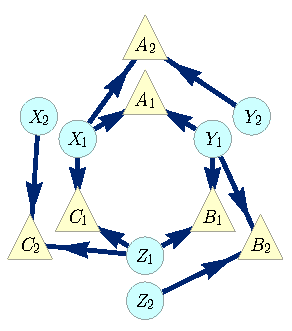
\includegraphics[scale=1]{TriDagSub222fixedcoordALT.pdf}
\caption{A relevant inflation of the Triangle scenario. (Repeat of \cref{fig:Tri222}.)}\label{fig:Tri222v2}
\end{minipage}
\end{figure}


Consider another causal inference problem concerning the Triangle scenario, namely, that of determining whether the hypothesis of the Triangle DAG is compatible with a joint distribution 
%$P^{\text{W}}_{A B C}$
$P_{A B C}$ of the form
\begin{align}\label{eq:wdistribution1}
P_{A B C}=\frac{[100]+[010]+[001]}{3},\quad\text{i.e.,}\quad P_{A B C}(a b c)=\begin{cases}\tfrac{1}{3}&\text{if }\; a\cramp{+}b\cramp{+}c\eql 1, \\ 0&\text{otherwise}.\end{cases}
\end{align}
We call this the W-type distribution\footnote{Because its correlations are reminiscent of those one obtains for the quantum state appearing in~\cite{3Qubits2Ways}, called the \emph{W state}.}. 
%To our knowledge, the fact that the Triangle causal structure is inconsistent with the W-type distribution has not been demonstrated previously.

To settle the compatibility question, we consider the inflated DAG of \cref{fig:Tri222v2}.  The injectable sets in this case include $\{A_1 B_1 C_1\}$, $\{A_2 C_1\}$, $\{B_2 A_1\}$, $\{C_2 B_1\}$,  $\{A_2\}$, $\{B_2\}$ and $\{C_2\}$. 

Therefore, we turn our attention to determining whether the marginals of the W-type distribution on the images of these injectable sets are compatible with the Triangle hypothesis.  These marginals are:
\begin{align}
P_{A B C}&= \frac{[100]+[010]+[001]}{3}, \label{V4}\\
P_{A C}= P_{B A} = P_{C B} & = \frac{[10]+[01]+[00]}{3}, \label{V1}\\
P_{A}= P_B = P_C & = \frac{2}{3}[0] + \frac{1}{3}[1]. \label{V5}
\end{align}

But by \cref{mainlemma}, this compatibility holds only if the corresponding set of marginals is compatible with the inflated DAG depicted in~\cref{fig:Tri222v2}:
\begin{align}
P_{A_1 B_1 C_1}&= \frac{[100]+[010]+[001]}{3}, \label{W4}\\
P_{A_2 C_1} = P_{B_2 A_1} = P_{C_2 B_1} & = \frac{[10]+[01]+[00]}{3}, \label{W1}\\
P_{A_2} = P_{B_2} = P_{C_2} & = \frac{2}{3}[0] + \frac{1}{3}[1]. \label{W5}
\end{align}

\begin{comment}
\color{purple} 
%Eq.~\eqref{W1} implies that one never has $A_2 \eql 1$ and $C_1\eql 0$, Eq.~\eqref{W2} implies that one never has $B_2 \eql 1$ and $A_1\eql 0$, and Eq.~\eqref{W3} implies that one never has $C_2 \eql 1$ and $B_1\eql 0$.  Similarly, Eq.~\eqref{W4} implies that one never has $A_1 =1$,  $B_1 =1$ and $C_1 =1$. 
From Eqs.~\eqref{W1}, \eqref{W2} and \eqref{W3}  respectively, one infers that one never has $A_2 \eql 1$ and $C_1\eql 0$, one never has $B_2 \eql 1$ and $A_1\eql 0$, and one never has $C_2 \eql 1$ and $B_1\eql 0$. Similarly, Eq.~\eqref{W4} implies that one never has $A_1 =0$,  $B_1 =0$ and $C_1 =0$.  From the latter constraint one infers that at least one of $A_1$, $B_1$ and $C_1$ must be 1, which from the former constraints implies that at least one of $A_2$, $B_2$ and $C_2$ must be 0, so that it is not the case that all of $A_2$, $B_2$ and $C_2$ are 1.

Recasting this argument in logical notation, where $\land$, $\lor$ and $\lnot$ denote conjunction, disjunction and negation respectively, the marginal distributions imply the truth of the following conjunction:
%We can therefore infer the truth of the conjunction of these claims, which can be expressed in logical notation as:
%a particular conjunction of events, namely, it implies the truth of
\begin{align}
\lnot [A_2 =1 \land C_1 =1] \land \lnot [B_2 =1 \land A_1 =1] \land \lnot [C_2 =1 \land B_1 =1] \land \lnot [A_1 =1 \land B_1 =1 \land C_1 =1],
\end{align}
and this logically implies the truth of
\begin{align}\label{consequent}
\lnot [A_2 =1 \land B_2 =1 \land C_2 =1].
\end{align}

However, our inflated DAG is such that $A_2$,$B_2$, and $C_2$ have no common ancestor and consequently, they are all marginally independent in any distribution consistent with this DAG.  This fact, together with Eqs.~\eqref{W5}-\eqref{W7}, implies that $A_2$,$B_2$, and $C_2$ sometimes all take the value 1, which contradicts \cref{consequent}.

Consequently, the set of marginals described in Eqs.~\eqref{W4}-\eqref{W7} are \emph{not} compatible with the DAG of Fig.~\ref{fig:Tri222v2}.  By \cref{mainlemma}, this implies that the set of marginals described in Eqs.~\eqref{V4}-\eqref{V7}---and therefore the W-type distribution of which they are marginals---is not compatible with the DAG of the Triangle scenario.
\color{black}
\end{comment}


\cref{W1} %together with the form of $P_{\text{W}}$ 
implies that $C_1\eql 0$ whenever $A_2 \eql 1$. It also implies that $A_1\eql 0$ whenever $B_2\eql 1$, and that $B_1\eql 0$ whenever $C_2\eql 1$, 
%, that is, $A_2=1$ and $B_2=1$ and $C_2=1$.  
%Summarizing, we have
\begin{align} 
\begin{split}\label{Ws}
&A_2 \eql 1 \implies C_1\eql 0,\\
&B_2\eql 1 \implies A_1\eql 0,\\
&C_2 \eql 1 \implies B_1 \eql 0.
\end{split}
\end{align}

Our inflated DAG is such that $A_2$, $B_2$ and $C_2$ have no common ancestor and consequently, they are all marginally independent in any distribution consistent with this inflated DAG.  This fact, together with \cref{W5}, implies that %$A_2$,$B_2$, and $C_2$ sometimes all take the value 1,
\begin{align} \label{WW2}
\text{Sometimes} \quad &A_2 \eql 1\,\text{ and }\, B_2 \eql 1\,\text{ and }\, C_2 \eql 1.
\end{align} 
Finally, \cref{Ws} together with \cref{WW2} entails
\begin{align} \label{WW3}
\text{Sometimes} \quad &A_1 \eql 0\,\text{ and }\, B_1 \eql 0\,\text{ and }\, C_1 \eql 0.
\end{align}
This, however, contradicts~\cref{W4}.  Consequently, the set of marginals described in \cref{W4,W1,W5} are \emph{not} compatible with the DAG of~\cref{fig:Tri222v2}.  By \cref{mainlemma}, this implies that the set of marginals described in \cref{V4,V1,V5}---and therefore the W-type distribution of which they are marginals---is not compatible with the Triangle scenario.
% and the fact that $P_{\text{W}}$ has no weight on $[000]$.

To our knowledge, this has not been demonstrated previously. In fact, the incompatibility of the W-type distribution with the Triangle scenario cannot be derived via any of the following pre-existing causal inference techniques:
\begin{compactenum}
\item Checking conditional independence relations is not relevant here, as there are \emph{no} conditional independence relations implied between any observable variables in the Triangle scenario. 
\item The relevant Shannon-type entropic inequalities for the Triangle scenario have been classified, and they do not witness the incompatibility either~\cite{fritz2013marginal,chaves2014novel,chaves2014informationinference}. 
\item Moreover, \emph{no} entropic inequality can witness the W-type distribution as unrealizable. \citet{weilenmann2016entropic} have constructed an inner approximation to the entropic cone of the Triangle causal structure, and the W-distribution lies inside this. In other words, a distribution with the same entropic profile as the W-type distribution \emph{can} arise from the Triangle scenario.
\item The newly-developed method of covariance matrix causal inference due to \citet{kela2016covariance}, which gives tighter constraints than entropic inequalities for the Triangle scenario, also cannot detect the incompatibility.
\end{compactenum}
%\par\noindent But the inflation technique can, and does so very easily.
Therefore, for this problem at least, the inflation technique appears to be more powerful. We have arrived at our incompatibility verdict by combining inflation with reasoning reminiscent of  Hardy's version of Bell's theorem~\cite{L.Hardy:PRL:1665,Mansfield2012}. \cref{sec:TSEM} will present a generalization of this kind of argument and its applications to causal inference. 

\example{: \tred{Witnessing the incompatibility of PR-box correlations with the Bell scenario}\label{example:noPR}}\par\smallskip\nobreak

Bell's theorem~\cite{bell1964einstein,Brunner2013Bell,bell1966lhvm,CHSHOriginal} concerns the question of whether the distribution obtained in an experiment involving a pair of systems that are measured at space-like separation is compatible with a causal structure of the form of \cref{fig:NewBellDAG1}. Here, the observed variables are $\brackets{A,B,X,Y}$, and $\Lambda$ is a latent variable acting as a common cause of $A$ and $B$. We shall term this causal structure the \emph{Bell scenario}. While the causal inference formulation of Bell's theorem is not the traditional one, several recent articles have introduced and advocated this perspective~[\citealp{WoodSpekkens}~(Fig.~19), \citealp{pusey2014gdag}~(Fig.~E\#2), \citealp{BeyondBellII}~(Fig.~1), \citealp{chaves2014novel}~(Fig.~1), \citealp{wolfe2015nonconvexity}~(Fig.~2b), \citealp{steeg2011relaxation}~(Fig.~2)].  

%Consider the causal structure associated to the Bell \cite{bell1964einstein,Brunner2013Bell,bell1966lhvm,CHSHOriginal} scenario [\citealp{pusey2014gdag}~(Fig.~E\#2), \citealp{WoodSpekkens}~(Fig.~19), \citealp{chaves2014novel}~(Fig.~1), \citealp{BeyondBellII}~(Fig.~1), \citealp{wolfe2015nonconvexity}~(Fig.~2b), \citealp{steeg2011relaxation}~(Fig.~2)], depicted here in \cref{fig:NewBellDAG1}. The observable variables are $\brackets{A,B,X,Y}$, and $\Lambda$ is the latent common cause of $A$ and $B$. 

\begin{figure}[ht]
\centering
\begin{minipage}[t]{0.45\linewidth}
\centering
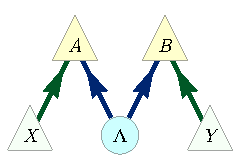
\includegraphics[scale=1]{BellDagRaw.pdf}
\caption{The causal structure of the bipartite Bell scenario. The local outcomes $A$ and $B$ of Alice's and Bob's measurements is assumed to be a function of some latent common cause and their independent local experimental settings $X$ and $Y$.}\label{fig:NewBellDAG1}
\end{minipage}
\hfill
\begin{minipage}[t]{0.45\linewidth}
\centering
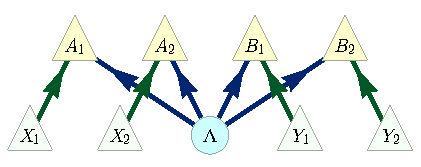
\includegraphics[scale=1]{BellDagCopy.pdf}
\caption{An inflated DAG of the bipartite Bell scenario, where both local settings and outcome variables have been duplicated.}\label{fig:BellDagCopy1}
\end{minipage}
\end{figure}

%P^{\text{obs-inf}}_{A_2 C_1}

We consider the distribution ${P_{A B X Y} = P_{A B | X Y} P_{X} P_{Y}}$, where $P_{X}$ and $P_{Y}$ are arbitrary full-support distributions\footnote{In the literature on the Bell scenario, these variables are known as ``settings''. Generally, we may think of endogenous observable variables as settings, coloring them light green in the DAG figures. Settings variables are natural candidates for conditioning on.} over the binary variables $X$ and $Y$, and
\begin{align}\begin{split}\label{eq:PRbox}
% & p_{\text{PR}}\parens{a b |x y}=\frac{[00|00]+[11|00]+[00|10]+[11|10]+[00|01]+[11|01]+[01|11]+[10|11]}{8}\\
P_{A B | X Y}\parens{a b |x y}=\begin{cases}\tfrac{1}{2}&\text{if }\; a + b \equiv x \cdot y \pmod{2}, \\ 0&\text{otherwise},\end{cases}
\end{split}\end{align}
a conditional distribution that was discovered by Tsirelson~\cite{Tsirelson1980} and later independently by Popescu and Rohrlich~\cite{PROriginal,PRUnit}. It has become known in the field of quantum foundations as the \emph{PR-box} after the latter authors.\footnote{The PR-box is of interest because it represents a manner in which experimental correlations could deviate from the predictions of quantum theory while still being consistent with relativity.}

%\color{purple} Recall that variables $X$ and $Y$ are conditionally independent given $Z,$ which we denote by $(X\indep Y\text{ }|\text{ }Z)$ if $P_{X,Y|Z}(xy|z) =P_{X|Z}(x|z) P_{Y|Z}(y|z) \qquad\forall z: P(Z=z)>0.$ \color{black}

The Bell scenario implies nontrivial conditional independences among the observed variables, namely, $X \indep Y$, $A \indep Y| X$, and\footnote{Recall that variables $X$ and $Y$ are conditionally independent given $Z$ if $P_{X,Y|Z}(xy|z) = P_{X|Z}(x|z) P_{Y|Z}(y|z)$ for all $z$ with $P_{Z}(z)>0$. Such a conditional independence is denoted by $X\indep Y\text{ }|\text{ }Z$.} $B \indep X|Y$, as well as those that can be generated from these by the semi-graphoid axioms \cite{WoodSpekkens}.
%We will use the inflation technique to show that this distribution is incompatible with the Bell scenario.
(In the context of a Bell experiment, where $\{X,A\}$ are space-like separated from $\{Y,B\}$, the conditional independences $A \indep Y| X$, and $B \indep X|Y$ encode the impossibility of sending signals faster than the speed of light.) It is straightforward to check that these conditional independence relations are respected by the $P_{ABXY}$ resulting from~\cref{eq:PRbox}. It is well-known that this distribution is nonetheless incompatible with the Bell scenario, for example since it violates the CHSH inequality.
%, and they are well-known to be incompatible with the Bell scenario \cite{PROriginal,PRUnit}. 
%Here we prove the incompatibility using the inflation technique. 
Here we prove this incompatibility via the inflation technique, using the inflation shown in \cref{fig:BellDagCopy1}.

We begin by noting that $\{A_1 B_1 X_1 Y_1\}$, $\{A_2 B_1 X_2 Y_1\}$, $\{A_1 B_2 X_1 Y_2\}$, $\{A_2 B_2 X_2 Y_2\}$, $\{X_1\}$, $\{X_2\}$, $\{Y_1\}$, and $\{Y_2\}$ are all injectable sets. 
By \cref{mainlemma}, it follows that any causal model that recovers $P_{ABXY}$ inflates to a model that results in marginals
\begin{align}
P_{A_1 B_1 X_1 Y_1}=P_{A_2 B_1 X_2 Y_1}=P_{A_1 B_2 X_1 Y_2}=P_{A_2 B_2 X_2 Y_2}&=P_{A B X Y},\label{PR1}\\
P_{X_1}=P_{X_2}=P_X, \qquad P_{Y_1}=P_{Y_2}&=P_Y.\label{PR5}
\end{align}
Using the definition of conditional probability, we infer that
\begin{align}
P_{A_1 B_1 |X_1 Y_1}=P_{A_2 B_1 |X_2 Y_1}=P_{A_1 B_2 |X_1 Y_2}=P_{A_2 B_2 |X_2 Y_2}=P_{A B |X Y}\label{PRb}.
\end{align}
Because $\{X_1\}$, $\{X_2\}$, $\{Y_1\}$, and $\{Y_2\}$ have no common ancestor in the inflated DAG, these variables must be marginally independent in any distribution compatible with the inflated DAG. This applies in particular to the inflation model, so that $P_{X_1 X_2 Y_1 Y_2} = P_{X_1} P_{X_2} P_{Y_1} P_{Y_2}$. Given the assumption that the distributions $P_{X}$ and $P_{Y}$ are full support, it follows from~\cref{PR5} that
\begin{align}\label{PRs}
\text{Sometimes} \quad &X_1 = 0, X_2 \eql1, Y_1 \eql 0, Y_2 \eql 1.
\end{align} 
On the other hand, from~\cref{PRb} together with  the definition of PR-box,~\cref{eq:PRbox}, we conclude that 
\begin{align} 
\begin{split}
\label{PRsi}
&X_1 \eql 0, Y_1 \eql 0 \implies A_1\eql B_1,\\
&X_1 \eql 0, Y_2 \eql 1 \implies A_1\eql B_2,\\
&X_2 \eql 1, Y_1 \eql 0 \implies A_2\eql B_1,\\
&X_2 \eql 1, Y_2 \eql 1 \implies A_2\ne B_2.
\end{split}
\end{align}
Combining this with~\cref{PRs}, we obtain
\begin{align}
\text{Sometimes} \quad &A_1\eql B_1, A_1\eql B_2, A_2\eql B_1, A_2\ne B_2.
\end{align} 
No values of $A_1, A_2, B_1, B_2$ can jointly satisfy these conditions---the first three entail perfect correlation between $A_2$ and $B_2$, while the fourth entails perfect anti-correlation---so we have reached a contradiction, showing that our original assumption of compatibility between $P_{ABXY}$ and the Bell scenario must have been false.

%For these values, \cref{eq:PRinflated} specifies perfect correlation between $A_1$ and $B_1$.  Similarly, it the inflated observational data also specified perfect correlation between $A_1$ and $B_2$, perfect correlation between $A_2$ and $B_1$, and perfect \emph{anti}correlation between $A_2$ and $B_2$. Those four requirements are not mutually compatible, however: since perfect correlation is transitive, the first three properties entail perfect correlation between $A_2$ and $B_2$. 

The structure of this proof parallels that of standard proofs of the incompatibility of the PR-box with the Bell DAG. Standard proofs focus on a set of variables $\{A_0, A_1, B_0, B_1\}$ where $A_x$  is the value of $A$ when $X=x$ and $B_y$  is the value of $B$ when $Y=y$, and note that  the distribution
%if the Bell DAG describes the experiment, then by taking 
%the product of the probability of each of these four variables given $\lambda$, that is,
 $\sum_{\lambda} P(A_0|\lambda)P(A_1|\lambda)P(B_0|\lambda)P(B_1|\lambda)P(\lambda)$
 %(the probability of $A_0$ given $\lambda$, of $A_1$ given $\lambda$, etcetera, one obtains 
 is a joint distribution over $\{A_0, A_1, B_0, B_1\}$ for which the marginals on pairs  $\{ A_0, B_0\}$, $\{ A_0, B_1\}$, $\{ A_1, B_0\}$ and $\{ A_1, B_1\}$ are those predicted by the Bell DAG.  Finally, the existence of such a joint distribution rules out the possibility of having $A_1\eql B_1, A_1\eql B_2, A_2\eql B_1$ but $ A_2\ne B_2$ and therefore shows that the PR Box correlations are incompatible with the Bell DAG \cite{LSW,roberts_thesis}. In light of our use of \cref{PRs}, our reasoning is really the same argument in disguise.

\cref{sec:Bellscenarios} shows that the inflation of~\cref{fig:BellDagCopy1}, with the number of copies corresponding to the cardinality of $X$ and $Y$, is enough to witness the incompatibility of any distribution that is indeed incompatible with the Bell scenario.

%  Finally, these marginals are shown to satisfy a Bell inequality, while the PR box correlations are shown to violate this inequality.   \purp{Is there a ``standard proof'' that excludes PR box without referring to Bell inequalities? Say something about the difference of the standard approach to our approach?---RWS}

% The fact that there must be a joint distribution over these variables can be inferred from the structure of the Bell DAG and the fact that one can assume without loss of generality that the causal dependences are deterministic (a result known as Fine's theorem \cite{FineTheorem}).  It is then sufficient to note that the marginals given by the PR-box correlations do not arise from any joint distribution.  Nonetheless, our proof is conceptually distinct insofar as the variables to which we apply the marginal problem are not conditioned on a setting value.  And we do not require Fine's theorem.  

%Many causal inference techniques can be used to derive sufficient conditions for the incompatibility of the causal hypothesis $H_{G',S'}$ with the observational data $\forall \bm{U} \in \SmallNamedFunction{PreInjectableSets}{\bm{O}}: \pdf{\bm{U}} = \pdf{\subsim{\bm{U}_1}}\pdf{\subsim{\bm{U}_2}} \dots \pdf{\subsim{\bm{U}_n}}$. We will call sets of such conditions \tblue{incompatibility witnesses}.   


%\subsection{Deriving causal compatibility inequalities using the inflation technique}\label{Sec:DerivingInequalities}
\subsection{Deriving causal compatibility inequalities}\label{Sec:DerivingInequalities}

The inflation technique can be used not only to witness the incompatibility of a given distribution with a given causal structure, but also to derive generally applicable necessary conditions that a distribution must satisfy to be compatible with the given causal structure. When these conditions are expressed as inequalities, we will refer to them as {\em causal compatibility inequalities}.  Formally, we have:

\begin{definition}
Let $G$ be a causal structure and $S \subseteq \SmallNamedFunction{ObservedNodes}{G}$.  Let $I_S$ denote an inequality that operates on a families of marginal distributions  $\{ P_{\bm{U}}: \bm{U} \in S\}$.  Then $I_S$ is a \tblue{\em causal compatibility inequality for the causal structure $G$} whenever it is satisfied by every family of distributions $\{ P_{\bm{U}}: \bm{U} \in S\}$ that is compatible with $G$.
%Consider a DAG $G$ and a set of the observed nodes thereon, $S \subseteq \SmallNamedFunction{ObservedNodes}{G}$.  Let $I_S$ denote an inequality that is evaluated on a family of marginal distributions  $\{ P_{\bm{U}}: \bm{U} \in S\}$.  The inequality $I_S$ is termed a \tblue{\em causal compatibility inequality for the DAG $G$} whenever it is satisfied by every family of distributions $\{ P_{\bm{U}}: \bm{U} \in S\}$ that is compatible with the DAG $G$.
\end{definition}
%\begin{definition}
%Consider a set of distributions over subsets of observed nodes on a DAG $G$, $\{ P_{\bm{U}}: \bm{U} \in \SmallNamedFunction{Subsets}{\SmallNamedFunction{ObservedNodes}{G}}\}$.  An inequality on such a set of distributions, denoted $I(\{ P_{\bm{U}}: \bm{U} \in \SmallNamedFunction{Subsets}{\SmallNamedFunction{ObservedNodes}{G}}\} )$, is termed a {\em causal compatibility inequality} just in case it is satisfied  whenever $\{ P_{\bm{U}}: \bm{U} \in \SmallNamedFunction{Subsets}{\SmallNamedFunction{ObservedNodes}{G}}\}$ is compatible with the DAG.  
%\end{definition}
While violation of a causal compatibility inequality witnesses the incompatibility of a distribution with the associated causal structure, the inequality being satisfied does not guarantee that the distribution is compatible with the causal structure.  This is the sense in which it merely provides a {\em necessary} condition for compatibility. 

The inflation technique is useful for deriving causal compatibility inequalities because of the following consequence of  \cref{mainlemma}:
%\begin{corollary} \label{maincorollary}
%Let $G$ and $G'$ be DAGs, with $G'$ an inflation of $G$.  Consider a set of distributions on the injectable sets on $G'$, denoted $S' := \{ P'_{\bm{U}'} : \bm{U}' \in \SmallNamedFunction{InjectableSets}{G'} \}$.  Consider also a set of distributions on the images of these injectable sets on $G$, denoted $S :=  \{ P_{\bm{U}} : \bm{U} \in \SmallNamedFunction{ImagesInjectableSets}{G} \}$.    Let $I'(S')$ be an inequality on $S'$, and let $I(S)$ be the inequality on $S$ that is obtained from $I'(S')$ as follows: for each injectable set $\bm{U'}$, replace $P'_{\bm{U}'}$ with $P_{\bm{U}}$ in $I'(S')$.  In this case, if $I'(S')$ is a causal compatibility inequality for the DAG $G'$ then $I(S)$ is a causal compatibility inequality for the DAG $G$.
%\end{corollary}

\begin{corollary} \label[corollary]{maincorollary}
Suppose that $G'$ is an inflation of $G$. Let $S'  \subseteq \SmallNamedFunction{InjectableSets}{G'}$ be a family of injectable sets and $S \subseteq \SmallNamedFunction{ImagesInjectableSets}{G}$ the images of members of $S'$.
%Let $S'$ be a family of injectable sets on $\SmallNamedFunction{ObservedNodes}{G'}$, $S'  \subseteq \SmallNamedFunction{InjectableSets}{G'}$, and let $S$ be the image on $\SmallNamedFunction{ObservedNodes}{G}$ of this family, $S \subseteq \SmallNamedFunction{ImagesInjectableSets}{G} \}$.    
%Consider a family of marginal distributions on the elements of $S$, $\{ P_{\bm{U}} : \bm{U} \in S\}$, whose marginals are consistent on the places where the elements of $S$ overlap. 
Let $I_{S'}$ be a causal compatibility inequality for $G'$ operating on families $\{ P_{\bm{U}'} : \bm{U}' \in S'\}$. Define an inequality $I_S$ as follows: in the functional form of $I_{S'}$, replace every occurrence of a term $P_{\bm{U}'}$ by $P_{\bm{U}}$ for the unique $\bm{U}\in S$ with $\bm{U} \sim \bm{U}'$. Then $I_S$ is a causal compatibility inequality for $G$ operating on families $\{ P_{\bm{U}} : \bm{U}\in S\}$.
\end{corollary}

The proof is as follows.  Suppose that the family $\{ P_{\bm{U}} : \bm{U} \in S\}$ is compatible with $G$.  By \cref{mainlemma}, it follows that the family $ \{ P_{\bm{U}'} : \bm{U}' \in S'\}$ where $P_{\bm{U}'}:= P_{\bm{U}}$ for $\bm{U}' \sim \bm{U}$  is compatible with $G'$.  Given that $I_{S'}$ is assumed to be a causal compatibility inequality for $G'$, it follows that $\{ P_{\bm{U}'} : \bm{U}' \in S'\}$ satisfies $I_{S'}$.  But by the definition of $I_{S}$, its evaluation on $\{ P_{\bm{U}} : \bm{U} \in S\}$ is equal to $I_{S'}$ evaluated on $\{ P_{\bm{U}'} : \bm{U}' \in S'\}$. Since $\{ P_{\bm{U}'} : \bm{U}' \in S'\}$ satisfies $I_{S'}$, it therefore follows that $\{ P_{\bm{U}} : \bm{U} \in S\}$ satisfies $I_{S}$. Since $\{ P_{\bm{U}} : \bm{U}\in S\}$ was an arbitrary family compatible with $G$, it follows that $I_{S}$ is a causal compatibility inequality for $G$.  

%\color{red} [No!  we can't have if and only if for the DAG G'.  If we have it at all, it's for the causal hypothesis that includes the parameter constraints. ]\color{black}

%\begin{corollary} Let $G$ and $G'$ be DAGs with $G'$ an inflation of $G$. 
%Consider the set of distributions on the injectable sets on $G'$ [...] and the set of distributions on the images on $G$ of the injectable sets on $G'$ [...]   Let $f'(...) \le C$ be an inequality on [...], where $f'$ is a function on [...] and $C$ is a constant.  Let $f(...)$ be the function on [...] that is obtained as follows: for each injectable set $\bm{U'}$, replace $P'_{\bm{U}'}$ with $P_{\bm{U}}$ in $f'(...)$.  In this case, $f'(...) \le C$ is a causal compatibility inequality for the DAG $G'$ if and only if $f(...) \le C$ is a causal compatibility inequality for the DAG $G$.
%\end{corollary}

%\begin{corollary} Let $G$ and $G'$ be DAGs with $G'$ an inflation of $G$. 
%Consider the set of distributions on the injectable sets of observed variables [...] and the set of distributions on the images of the injectable sets of observed variables, [...]   Suppose that $f'(...) \le C$ for some function $f'$ and constant $C$ is a causal compatibility inequality for the DAG $G'$.  Let $f(...)$ be the function obtained by substituting $P_{\bm{U}}$ for $P_{\bm{U}'}$ in $f'(...)$ for each injectable set $\bm{U'}$.  Then $f(...) \le C$ is a causal compatibility inequality for the DAG $G$.
%\end{corollary}


%\subsection{Example applications of the inflation technique}\label{sec:examplebaddistributions}

%\color{red} Lemma: Consider a collection of sets of observed variables in the inflated DAG all of which are injectable. Any necessary condition for compatibility of a distribution with the inflated DAG that can be expressed entirely in terms of the marginals on these sets implies a necessary condition for compatibility of a distribution with the original DAG which is expressed in terms of the marginals on the images of these sets.  Formally, ....
%\color{black} 

We now present some simple examples of causal compatibility inequalities for the Triangle scenario that one can derive from the inflation technique via \cref{maincorollary}.

Some terminology and notation will facilitate the description of these examples. We refer to a pair of nodes which do not share any common ancestor as being \tblue{ancestrally independent}. This corresponds to being $d$-separated by the empty set~\cite{pearl2009causality,spirtes2011causation,studeny2005probabilistic,koller2009probabilistic}.  Given that the conventional notation for $X$ and $Y$ being $d$-separated by $Z$ in the DAG $G$ is $X\perp_G Y|Z$, we denote $X$ and $Y$ being ancestrally independent within $G$ as $X\perp_G Y$.  Generalizing to sets, $\bm{U}\aindep_G \bm{V}$ indicates that no node in $\bm{U}$ shares a common ancestor with any node in $\bm{V}$ within the DAG $G$, 
\begin{align}
\bm{U}\aindep_G \bm{V} \quad \text{iff} \quad \An[G]{\bm{U}}\cap\An[G]{\bm{V}}=\emptyset.
\end{align}
Furthermore, the notation ${\bm{U}\aindep_G \bm{V}\aindep_G \bm{W}}$ should be understood as indicating that $\bm{U}\aindep_G \bm{V}$ and $\bm{V}\aindep_G \bm{W}$ and $\bm{U}\aindep_G \bm{W}$.
% Ancestral independence is equivalent to $d$-separation by the empty set~\cite{pearl2009causality,spirtes2011causation,studeny2005probabilistic,koller2009probabilistic}. 

%Some terminology and notation will facilitate the description of these examples. We refer to a pair of nodes which do not share any common ancestor as being \tblue{ancestrally independent}, for which we invent the notation $X\aindep Y$. Generalizing to sets, $\bm{U}\aindep \bm{V}$ indicates that no node in $\bm{U}$ shares a common ancestor with any node in $\bm{V}$, 
%\begin{align}
%\bm{U}\aindep \bm{V} \quad \text{iff} \quad \An{\bm{U}}\cap\An{\bm{V}}=\emptyset.
%\end{align}
%Furthermore, the notation ${\bm{U}\aindep \bm{V}\aindep \bm{W}}$ should be understood as indicating that $\bm{U}\aindep \bm{V}$ and $\bm{V}\aindep \bm{W}$ and $\bm{U}\aindep \bm{W}$. Ancestral independence is equivalent to $d$-separation by the empty set~\cite{pearl2009causality,spirtes2011causation,studeny2005probabilistic,koller2009probabilistic}. 



\topic{\tred{Example of a causal compatibility inequality expressed in terms of \tpurp{\emph{correlators}}}}\smallskip\nobreak

As in \cref{example:noGHZ} of the previous section, consider the inflation of the Triangle scenario to the DAG depicted in~\cref{fig:TriDagSubA2B1C1v2}.  
The injectable sets we make use of here are $\brackets{A_2 C_1}$, $\brackets{B_1 C_1}$, $\{ A_2\}$, and  $\brackets{B_1}$.

From \cref{maincorollary}, any causal compatibility inequality for the inflated DAG that operates on the marginal distributions of $\brackets{A_2 C_1}$, $\brackets{B_1 C_1}$, $\{ A_2\}$, and  $\brackets{B_1}$ will yield a causal compatibility inequality for the original DAG that can evaluated on the marginal distributions for $\brackets{A C}$, $\brackets{B C}$, $\{ A\}$, and  $\brackets{B}$.
We begin, therefore by identifying a simple example of a causal compatibility inequality for the inflated DAG that is of this sort. 
 
In our example, all of the observed variables are binary. For technical convenience, we assume that these take values in the set $\{-1,+1\}$, rather than taking values in the set $\{0,1\}$ as was presumed in the last section. 

We begin by noting that for {\em any} distribution on three binary variables $\{A_2 B_1 C_1\}$, that is, {\em regardless} of the causal structure in which they are embedded, the marginals on $\brackets{A_2 C_1}$, $\brackets{B_1 C_1}$ and $\brackets{A_2 B_1}$ satisfy the following inequality for expectation values~\cite{pitowsky_boole_1994,Pitowsky1989,kellerer_marginal_1964,leggett_garg_1985,araujo_cycle_2013},
\begin{equation}
	\label{eq:polymonogamyraw}
	\langle A_2 C_1\rangle + \langle B_2 C_1 \rangle - \langle A_2 B_1 \rangle \leq 1.
\end{equation}
This is an example of a constraint on pairwise correlators that arises from the presumption that they are consistent with a joint distribution. (The problem of deriving such constraints is the so-called {\em marginal problem}, dicussed in detail in \cref{sec:ineqs}.)

But the DAG of~\cref{fig:TriDagSubA2B1C1v2} shows that $A_2$ and $B_1$ have no common ancestor and consequently any distribution compatible with the DAG must make $A_2$ and $B_1$ marginally independent.  In terms of correlators, this can be expressed as 
%means that 
\begin{align}\label{corrfact}
A_2 \aindep B_1 \implies  \langle A_2 B_1 \rangle =  \langle A_2\rangle \langle B_1 \rangle.
\end{align}
Substituting the latter equality into~\cref{eq:polymonogamyraw}, we have
\begin{equation}
	\langle A_2 C_1\rangle + \langle B_2 C_1 \rangle   \leq 1 + \langle A_2 \rangle \langle B_1\rangle.
\end{equation}
This is an example of a simple but nontrivial causal compatibility inequality for the DAG of~\cref{fig:TriDagSubA2B1C1v2}.  

Finally, by \cref{maincorollary} and the fact that the DAG of~\cref{fig:TriDagSubA2B1C1v2} is an inflation of the Triangle scenario, we infer that 
%\begin{equation}
%	\langle A C\rangle + \langle B C \rangle - \langle A \rangle \langle B \rangle \leq 1.
%\end{equation}
\begin{equation}
	\label{eq:polymonogamy}
	\langle A C\rangle + \langle B C\rangle \leq 1 + \langle A\rangle \langle B\rangle,
\end{equation}
is a causal compatibility inequality for the Triangle scenario.   This inequality expresses the fact that as long as $A$ and $B$ are not completely biased, there is a tradeoff between the strength of $AC$ correlations and the strength of $BC$ correlations.   

Given the symmetry of the Triangle scenario under permutations and sign flips of $A$, $B$ and $C$, it is clear that the image of inequality~\cref{eq:polymonogamy} under any such symmetry is also a valid causal compatibility inequality.  Together, these inequalities imply monogamy\footnote{We are here using the term ``monogamy'' in the same sort of manner in which it is used in the context of entanglement theory~\cite{horo4}.}  of correlations in the Triangle scenario with binary variables:  if any two observed variables with unbiased marginals are perfectly correlated, then they are both uncorrelated with the third.


%This inequality expresses a trade-off in the strength of the correlations that can be observed between any pair of observed nodes in the Triangle scenario: at most two such pairs can be perfectly correlated. %\purp{Is this an accurate description of the constraint?  I don't see how to justify calling it ``monogamy".  ---RWS}

%must be monogamous:  if $A$ and $B$ are strongly correlated 
%we think of as a sort of monogamy inequality: it is impossible for $C$ to be strongly correlated with both $A$ and $B$, unless $A$ and $B$ are both strongly biased.

\topic{\tred{Example of a causal compatibility inequality expressed in terms of \tpurp{\emph{entropic quantities}}}}\smallskip\nobreak

One way to derive constraints that are independent of the cardinality of the observed variables is to express these in terms of the mutual information between observed variables rather than in terms of correlators.  The inflation technique can also be applied to achieve this.
%Inequalities expressed in terms of entropies and mutual information (rather than correlators) have the advantage that one can easily derive constraints that are independent of the cardinality of the observed variables.  
%This is the case with the inflation technique as well.  
To see how this works in the case of the Triangle scenario, consider again the inflated DAG of~\cref{fig:TriDagSubA2B1C1v2}.  

One can follow the same logic as in the preceding example, but starting from a different constraint on marginals.  For any distribution on three variables $\{A_2 B_1 C_1\}$ of arbitrary cardinality (again, regardless of the causal structure in which they are embedded), the marginals on $\brackets{A_2 C_1}$, $\brackets{B_1 C_1}$ and $\brackets{A_2 B_1}$ satisfy the inequality~\cite[Eq.~(29)]{fritz2013marginal}
\begin{align}\label{eq:MIraw}
	I(A_2 : C_1) + I(C_1 : B_1) - I(A_2 : B_1) \leq H(C_1),	
\end{align}
where $H(X)$ denotes the Shannon entropy of the distribution of $X$, and $I(X: Y)$ denotes the mutual information between $X$ and $Y$ with respect to the marginal on $X$ and $Y$.

The fact that $A_2$ and $B_1$ have no common ancestor in the inflated DAG implies that in any distribution that is compatible with the inflated DAG, $A_2$ and $B_1$ are marginally independent.  This is expressed entropically as the vanishing of their mutual information, 
\begin{align}\label{entropicfact}
A_2 \aindep B_1 \implies  I(A_2 : B_1)  =0.
\end{align}
Substituting the latter equality into~\cref{eq:MIraw}, we have
\begin{align}
	I(A_2 : C_1) + I(C_1 : B_1)  \leq H(C_1).
\end{align}
This is another example of a nontrivial causal compatibility inequality for the DAG of~\cref{fig:TriDagSubA2B1C1v2}.  

By \cref{maincorollary}, it follows that 
\begin{align}\label{eq:monogomyofcorrelations}
	I(A : C) + I(C : B) \leq H(C),
\end{align}
is also a causal compatibility inequality for the Triangle scenario.  This inequality was originally derived in~\cite{fritz2012bell}. Our rederivation in terms of inflation coincides with the proof found by~\citet{pusey2014gdag}.

%To see how this distribution is incompatible with \cref{eq:tritrivial1}, note that for three \emph{identically distributed} (but not independent) binary variables a further special case of \cref{eq:tritrivial1} is
%\begin{align*}\begin{split}
%&\hspace{-6ex}3\p{A\cramp{=}1}\leq 1+\p{A\cramp{=}1}^2+2\p{A\cramp{=}B\cramp{=}1}.
%\end{split}\end{align*}
%For the W-distribution ${\p{A\cramp{=}B\cramp{=}C\cramp{=}0}=0}$, and also ${\p{A\cramp{=}1,B\cramp{=}1}=0}$, yet ${\p{A\cramp{=}1}=\nicefrac{1}{3}}$. As ${(\nicefrac{1}{3})^3\nleq 0}$ we have proven that the W-type distribution is incompatible with the Triangle scenario.
%Earlier works have already shown that the GHZ-type distribution is incompatible with the classical Triangle scenario \cite{steudel2010ancestors,fritz2012bell,chaves2014novel}. Interestingly, however, the entropic monogamy relation $I\parens{A:B}+I\parens{A:C}\leq H\parens{A}$ which rejects the GHZ-type distribution has been shown also to hold if the hidden shared resources are non-classical, even using generalized probabilistic theories \cite[Cor. 24]{pusey2014gdag}. 


\bigskip

\topic{\tred{Example of a causal compatibility inequality expressed in terms of \tpurp{\emph{probabilities}}  of certain joint valuations}}\smallskip\nobreak



Consider the inflation of the Triangle scenario depicted in~\cref{fig:Tri222v2}, with the injectable sets $\{A_1 B_1 C_1\}$, $\{A_1 B_2\}$, $\{B_1 C_2\}$, $\{ A_1, C_2\}$, $\{A_2\}$, $\{B_2\}$, and $\{C_2\}$.
%.  The injectable sets in this case include $\{A_1 B_1 C_1\}$, $\{A_1 B_2\}$, $\{B_1 C_2\}$, $\{ A_1, C_2\}$, $\{A_2\}$, $\{B_2\}$, and $\{C_2\}$.  
We here derive a causal compatibility inequality under the assumption that the observed variables are binary, adopting the convention that they take values in $\{0,1\}$.

We begin by noting that the following is a constraint that holds for any joint distribution of $\{A_1 B_1 C_1 A_2 B_2 C_2\}$, regardless of the causal structure, 
\begin{align}\label{eq:FritzF3raw}
	P_{A_2 B_2 C_2}(111) \leq P_{A_1 B_1 C_1}(000) + P_{A_1 B_2 C_2}(111) + P_{B_1 C_2 A_2}(111) + P_{A_2  C_1 B_2}(111).
	% Mermin: \langle A_1 B_1 C_1 \rangle - \langle A_2 B_2 C_1 \rangle - \langle A_2 B_1 C_2 \rangle - \langle A_1 B_2 C_2 \rangle \leq 2.
\end{align}
To prove this claim, it suffices to check that the inequality holds for each of the $2^6$ deterministic assignments of values to $\{A_1 B_1 C_1 A_2 B_2 C_2\}$, from which the general case follows by linearity.  A more intuitive proof will be provided in~\cref{sec:TSEM}.

Next, we note that certain sets of variables have no common ancestors with other sets of variables in the inflated DAG, and we infer the marginal independence of the two sets, expressed now as a factorization of a joint distribution,
%which is expressed as the factorization of the distributions over these variables,
\begin{align}\begin{split}\label{eq:tri222fac}
%P_{A_1 B_1 C_1} &= P_{A B C}, \\
A_1 B_2 \aindep C_2 \implies	P_{A_1 B_2 C_2} &= P_{A_1 B_2} P_{C_2}, \\
B_1 C_2 \aindep A_2 \implies	P_{B_1 C_2 A_2} &= P_{B_1 C_2} P_{A_2}, \\
A_2 C_1 \aindep B_2 \implies	P_{A_2 C_1 B_2} &= P_{A_2 C_1} P_{B_2}, \\
A_2 \aindep B_2 \aindep C_2 \implies	P_{A_2 B_2 C_2} &= P_{A_2} P_{B_2} P_{C_2} .
\end{split}\end{align}
Substituting these equations into~\cref{eq:FritzF3raw}, we obtain the polynomial inequality
\begin{equation}%\label{eq:FritzF3}
	P_{A_2}(1) P_{B_2}(1) P_{C_2}(1) \leq P_{A_1 B_1 C_1 }(000) + P_{A_1 B_2}(11) P_{C_2}(1) + P_{B_1 C_2}(11) P_{A_2}(1) + P_{A_2 C_1}(11) P_{B_2}(1).
	% Mermin-poly: \langle A B C\rangle \leq 2 + \langle A B\rangle \langle C\rangle + \langle B C \rangle \langle A\rangle + \langle C A\rangle \langle B\rangle,
\end{equation}
This, therefore, is a causal compatibility inequality for the DAG of ~\cref{fig:Tri222v2}. Finally, by \cref{maincorollary}, we infer that 
\begin{equation}\label{eq:FritzF3}
	P_{A}(1) P_{B}(1) P_{C}(1) \leq P_{ABC}(000) + P_{AB}(11) P_C(1) + P_{BC}(11) P_A(1) + P_{AC}(11) P_B(1)
	% Mermin-poly: \langle A B C\rangle \leq 2 + \langle A B\rangle \langle C\rangle + \langle B C \rangle \langle A\rangle + \langle C A\rangle \langle B\rangle,
\end{equation}
is a causal compatibility inequality for the Triangle scenario.  

What is distinctive about this inequality is that---through the presence of the term $P_{ABC}(000)$---it takes into account genuine three-way correlations.  This inequality is strong enough to demonstrate the incompatibility of the W-type distribution of \cref{eq:wdistribution1} with the Triangle scenario: for this distribution, the right-hand side of the inequality vanishes while the left-hand side does not.
% \cref{eq:FritzF3} requires the use of a broadcasting inflation, and therefore does not hold in the context of general probability theories.
%, where $a,b,c\in\brackets{0,1}$.
%The W-distribution states that the in any event in which $A,B,C$ are observed, precisely one of them will be found to equal $1$ while the other two will equal $0$. The identity of the variable which takes the value $1$ is uniformly random. In informal but intuitive notation, the W-type distribution is ${\nicefrac{1}{3}[100]+\nicefrac{1}{3}[010]+\nicefrac{1}{3}[001]}$.
%To see how this distribution is incompatible with \cref{eq:FritzF3}, note that for three \emph{identically distributed} (but not independent) binary variables a further special case of \cref{eq:FritzF3} is
%\begin{align*}\begin{split}
%&\hspace{-6ex}\p{A\cramp{=}1}^3\leq \p{A\cramp{=}B\cramp{=}C\cramp{=}0} + 3\times\p{A\cramp{=}B\cramp{=}1}\p{C\cramp{=}1}.
%\end{split}\end{align*}
%For the W-distribution ${\p{A\cramp{=}B\cramp{=}C\cramp{=}0}=0}$, and also ${\p{A\cramp{=}1,B\cramp{=}1}=0}$, yet ${\p{A\cramp{=}1}=\nicefrac{1}{3}}$. As ${(\nicefrac{1}{3})^3\nleq 0}$ we have proven that the W-type distribution is incompatible with the Triangle scenario.

\bigskip

%\cref{sec:38ineqs} provides a list of further polynomial inequalities that we have derived for the Triangle scenario using the method developed in the following section.


Of the known techniques for witnessing the incompatibility of a distribution with a DAG or deriving necessary conditions for compatibility, the most straightforward is to consider the constraints implied by ancestral independences among the observed variables of the DAG. 
%There are many well-known tricks for witnessing the incompatibility of a distribution with a DAG or deriving necessary conditions for compatibility.  The absolutely most straightforward of these is to consider the ancestral independences in the DAG.   
The constraints derived in the last two sections have all made use of this basic technique, but at the level of the inflated DAG rather than the original DAG.  The constraints that one thereby infers for the original DAG reflect facts about its causal structure that cannot be expressed in terms of ancestral independences among its observed variables.  The inflation technique manages to expose these facts in the ancestral independences among observed variables of the inflated DAG.
%These facts can, however, be revealed in the ancestral independences among that are found in various inflations of the DAG.   In particular, facts about the original DAG that concern ancestral independences refering to {\em latent} variables \
%Such facts become exposed as ancestral independences among {\em observed variables} in the inflated DAG.
%``knows'' what allows the inflation technique to derive subtle constraints at the level of the original DAG from stra in these cases.  

%The inflation technique is such that by exploring such basic constraints at the level of the inflated DAG, one obtains more nuanced and subtle constraints at the level of the original DAG.  Because inflation tends to introduce ancestral independences than are not found in the original DAG

In the rest of this article, we shall continue to rely only on the ancestral independences among observed variables within the inflated DAG to infer compatibility constraints on the original DAG.   Nonetheless, it is possible that the inflation technique can also amplify the power of {\em other} techniques that do not merely consider ancestral independences among the observed variables.  We consider some prospects in \cref{sec:otherprospects}.
%   This question, however, is left for future research.
%any tricks that can be used to infer incompatibility or provide a necessary condition for compatibility in the inflation version of the problem can be used to infer incompatibility or provide a necessary condition for compatibility in the original version of the problem. 
%  The most straightforward of these tricks are to consider the ancestral independences in the inflated DAG.   Because inflation tends to introduce ancestral independences than are not found in the original DAG, even these most straightforward of tricks can be leveraged to obtain nontrivial constraints.  

%The fact that the inflated DAG often has ancestral independences which have no analogue in the original DAG, each of which has nontrivial consequences, is what makes the technique effective. 
% and which imply nontrivial consequences. 
%can be leveraged to infer incompability or provide necessary conditions for compatibility. 
%than were the original DAG is what provides novel opportunities for  deriving 
%has a richer structure tends to make for more such opportunites for easy constraints. 

%In all of these examples, the inequality with which one starts---a constraint upon marginals that is independent of the causal structure---involves sets of observed variables that are not all injectable.  Each of these sets can, however, be partitioned into disjoint subsets each of which {\em is} injectable where the partitioning represents ancestral independence in the inflated DAG.  It is useful to have a name for such sets of observed variables: we will call them {\em pre-injectable}.  We begin by defining this notion carefully before describing our general inflation technique. 
%\color{black}

\section{Systematically Witnessing Incompatibility and Deriving Inequalities}
\label{sec:ineqs}

%\subsection{Pre-injectable sets}

In the examples from the previous section, the initial inequality---a constraint upon marginals that is independent of the causal structure---involves sets of observed variables that are \emph{not} all injectable.  Each of these sets can, however, be partitioned into disjoint subsets each of which {\em is} injectable whenever the partitioning represents ancestral independence in the inflated DAG.   For instance, in the first example from the previous section, the set $\{ A_2 B_1\}$ can be partitioned into the singleton sets $\{ A_2 \}$ and $\{ B_1\}$ which are ancestrally independent and each of which is injectable.  It is useful to have a name for such sets of observed variables: we call them \tblue{pre-injectable}. So for a set of observable nodes $\bm{U}'$ in the inflated DAG $G'$,
\begin{align}\label{eq:defpreinj}
\bm{U}'\in\SmallNamedFunction{PreInjectableSets}{G'} \quad\text{ iff }\quad  \exists \{ \bm{U}_i \in \SmallNamedFunction{InjectableSets}{G'} \} \quad \text{s.t.}\quad \bm{U}'=\bigcup_i \bm{U}_i  \quad\text{and} \quad  \forall i\ne j: \bm{U}_i \aindep \bm{U}_j.
%\bm{U}\in\SmallNamedFunction{PreInjectableSets}{G'} \quad\text{ iff }\quad  \exists \{ \bm{U}_i \}_i \quad \text{s.t.}\quad \bm{U}=\bigcup_i \bm{U}_i  \quad\text{and} \quad \forall i 
%: \bm{U}_i \in \SmallNamedFunction{InjectableSets}{G'}\quad \text{and}\quad \forall i,j
%: \bm{U}_i \aindep \bm{U}_j.
\end{align}
%Equivalently, a set of nodes is pre-injectable if and only if its (weakly) connected components are injectable. 
For example, every injectable set is trivially a pre-injectable set.  A pre-injectable set is \emph{maximal} if it is not a proper subset of another pre-injectable set.

Because ancestral independence in the DAG implies statistical independence for any probability distribution compatible with the DAG, it follows that  if 
$\bm{U}'$ is a pre-injectable set and $\bm{U}_1,\ldots,\bm{U}_n$ are the ancestrally independent components of $\bm{U}'$, then 
\begin{align}\label{eq:preinjfactor}
%\forall \bm{U}\in\SmallNamedFunction{PreInjectableSets}{G'}:	
P_{\bm{U}'} = P_{\bm{U}_1} \cdots P_{\bm{U}_n}
\end{align}
for any distribution compatible with $G'$. The situation, therefore, is this: for any constraint that one can derive for the marginals on the pre-injectable sets based on the existence of a joint distribution---and hence without reference to the causal structure---one can infer constraints that {\em do} refer to the causal structure by substituting within these constraints factorizations of the form of~\cref{eq:preinjfactor}.  

Thus the pre-injectable sets play a crucial role in linking the original DAG with the inflation DAG: they are precisely those sets of variables whose joint distributions in an inflation model are fully specified by the original causal model on the original DAG: they can be computed using \cref{mainlemma} and \cref{eq:preinjfactor}. If the resulting family of marginal distributions on pre-injectable sets is not compatible with the existence of a joint distribution, then the original distribution is witnessed as causally incompatible with the original DAG. This is the formal argument underpinning all of the examples in \cref{subsec:witnessingincompat}.

The problem of determining constraints on marginals follows from the existence of a joint distribution is known as the {\em marginal problem}. Thus, we can summarize the situation as follows: an inequality derived from the marginal problem, after applying the factorizations of~\cref{eq:preinjfactor}, becomes a causal compatibility inequality for the inflated DAG. The latter inequality can then be converted into a polynomial causal compatibility inequality for the original DAG using \cref{maincorollary}.
%We have defined causal inference as a decision problem, namely testing the consistency of some observational data with some some causal hypothesis. We have shown that this decision can sometimes be negatively answered by proxy, namely by demonstrating inconsistency of \emph{inflated} data with an \emph{inflated} hypothesis. But the inflation technique is more useful than that: we can also derive explicit \emph{inequalities} that a distribution on observable nodes needs to satisfy in order to be compatible with the causal structure. % Any such constraint is also an implicit consequence of the original hypothesis, and hence a relevant infeasibility criterion.
This section considers the problem of how to implement this procedure systematically.



%In the discussion that follows, we continue to assume that the original hypothesis is nothing more than supposing the causal structure to be given by the original DAG. Furthermore we presume that the joint distribution over all original observable variables is accessible.

We limit our attention to deriving causal compatibility inequalities expressed in terms of probabilities\footnote{Or, for binary variables, equivalently in terms of correlators, as in the first example of \cref{Sec:DerivingInequalities}.}, as these are generally the most powerful. However, that the inflation technique can also be used to derive inequalities expressed in terms of entropies, as our second example from the previous section demonstrated. We show in \cref{sec:NonShannon} that the inflation technique implies the core lemma for deriving non-Shannon-type inequalities.

% The potential of using inflation as tool for deriving entropic inequalities is considered separately in \cref{sec:NonShannon}.

To obtain a complete solution of the marginal problem, one must determine all the facets of the \tblue{marginal polytope}, for which we discuss algorithms in~\cref{sec:projalgorithms}.
% The causal compatibility inequalities one thereby obtains are polynomial in the probabilities.  The rest of this section describes the steps for deriving all such inequalities.  
Computing all these facets is computationally costly.  It is therefore useful to also consider relaxations of the marginal problem that are less computationally burdensome by deriving valid linear inequalities which may or may not bound the marginal polytope tightly.
%Since computing all the facets of the marginal polytope is computationally costly, a useful simplification of the problem is to derive instead only a collection 
We describe one such approach based on possibilistic Hardy-type paradoxes and the hypergraph transversal problem. This strategy requires the least computational effort, but is limited in that it only yields inequalities of a very particular form.  We describe this approach in \cref{sec:TSEM}.


\begin{comment}
In what follows we consider three different strategies for constraining possible marginal distributions from the inflation hypothesis. 
\begin{compactitem}
\item The full nonlinear strategy attempts to leverage different kinds of constraints which follow from the inflation hypothesis. This strategy yields the strongest incompatibility witnesses, but relies on computationally-difficult nonlinear quantifier elimination.
\item An intermediate strategy asks only if the various marginal distributions are compatible with \emph{any} joint distribution, without regard to the specific causal structure of the inflated DAG whatsoever. Solving the marginal problem amounts to determining all the facets of the \tblue{marginal polytope}, for which we discuss algorithms in~\cref{sec:projalgorithms}. The resulting incompatibility witnesses are nevertheless still polynomial inequalities at the level of the original distribution.
\item Since computing all facets of the marginal polytope is computationally costly, one can try to derive instead only a collection of linear inequalities which bound it. One strategy for doing so is based on possibilistic Hardy-type paradoxes, which we connect to the hypergraph transversal problem. This strategy requires the least computational effort, but is limited in that it only yields polynomial inequalities of a very particular form.
\end{compactitem}

In the narrative below the marginal problem is discussed first; the nonlinear strategy is presented as supplementing the marginal problem with additional constraints. The most computationally efficient strategy is presented as a relaxation of the marginal problem, and is discussed separate from the other two strategies, namely in \cref{sec:TSEM}.
\end{comment}

Preliminary to every strategy is the identification of the pre-injectable sets, so we begin with this problem.

\subsection{Identifying the pre-injectable sets}\label{step:findpreinjectable}
%\topic{\tred{Identifying the Pre-Injectable Sets}}\label{step:findpreinjectable}

To identify the pre-injectable sets of an inflation DAG, we must first identify the injectable sets. This problem can be reduced to identifying the injectable pairs, because if all of the pairs in a set of nodes are injectable, then so too is the set itself.  The latter claim is proven as follows.   
%To prove this, it suffices to prove that if all of the pairs in a set of nodes are injectable, then so too is the set itself.  
Let $\varphi : G' \to G$ be the projection map from the inflated DAG $G'$ to
the original DAG $G$, corresponding to removing the copy-indices.  Then $\varphi$ has the characteristic feature that it takes edges to edges: if $A  \to B$ in $G'$, then also $\varphi(A) \to \varphi(B)$ in $G$. Conversely, if
$\varphi(A) \to \varphi(B)$ in $G$ then also $A \to B$ in $G'$; this follows from the
assumption that $G'$ is an inflation of $G$. 
%(It's secretly the *pair* (G',p) that is the inflation, but I think that we've already discussed that over lunch at some point.)
A set $\bm{U} \subseteq \SmallNamedFunction{ObservedNodes}{G'}$ is injectable if and only if the
restriction of $\varphi$ to the ancestors of $\bm{U}$ is an injective map. 
%This is simply a more formal way to state the definition of an injective set. 
%(Recall that U itself is considered included in its set of ancestors.)
But now injectivity of a map means precisely that no two different
elements of the domain get mapped to the same element of the codomain.
So if $\bm{U}$ is injectable, then so is each of its two-element subsets;
conversely, if $\bm{U}$ is not injectable, then $\varphi$ maps two nodes among the
ancestors of $\bm{U}$ to the same node, which means that there are two nodes in the
ancestry that differ only by copy index. Each of these two nodes must be
an ancestor of at least some node in $\bm{U}$; if one chooses two such
descendants, then one gets a two-element subset of $\bm{U}$ such that $\varphi$ is not
injective on the ancestry of that subset, and therefore this two-element
set of observed nodes is not injectable.
\color{black}

To enumerate the injectable sets, it is useful to encode certain features of the inflated DAG in an undirected graph which we call the \tblue{injection graph}. The nodes of the injection graph are the observed nodes of the inflated DAG, and a pair of nodes $A_i$ and $B_j$ share an edge if the pair $\{ A_i B_j\}$ is injectable. For example, \cref{fig:injection222} shows the injection graph of the inflation of \cref{fig:Tri222}.
 %$\An{A_i B_j}$ does not contain two distinct nodes that are equivalent up to copy index. 
The property noted above states that the injectable sets are precisely the cliques\footnote{A \emph{clique} is a set of nodes in an undirected graph any two of which share an edge.} of the injection graph.
%the injectable sets are characterized by the injection graph as follows.  
%a set of nodes in the inflated DAG is injectable if and only if the corresponding set of nodes in the injection graph forms a clique. 
%The injectable sets of the inflated DAG are the cliques of the injection graph. 
 % The injectable sets are then precisely the cliques\footnote{A clique is a subset of nodes such that every node in the subset is adjacent to every other node in the subset.} in this graph, per \cref{eq:definjectable}. 
While for many other other applications only the maximal cliques are of interest, our application of the inflation technique requires knowledge of all nonempty cliques. 
% Note that it is usually necessary to enumerate \emph{all} the nonempty cliques, i.e.~not only the maximal ones.

Given a list of the injectable sets, the pre-injectable sets can be read off from the \tblue{pre-injection graph}.
%Determining the pre-injectable sets from there can be done via constructing another graph that we call the \tblue{independence graph}. 
The nodes of the pre-injection graph are taken to be the injectable sets in $G'$, and two nodes share an edge if the associated injectable sets are ancestrally independent. %Then, by definition,
\cref{fig:preinjectiongraph222} depicts an example. 
The pre-injectable sets correspond to the cliques of the pre-injection graph: the union of all the injectable sets that make up the nodes of a clique is a pre-injectable set, while the individual nodes already give us the partition into injectable sets relevant for the factorization relation of \cref{eq:preinjfactor}. 
%represented by such a clique results in a pre-injectable set. 
For our purposes, it is sufficient to enumerate the maximal pre-injectable sets, so that one only needs to consider the maximal cliques of the pre-injection graph.
%Since it is sufficient to only consider the maximal pre-injectable sets, one can eliminate all those pre-injectable sets that are contained in other ones, as a final step.


%Let us also define the \tblue{ancestral dependence graph}, in which two nodes are adjacent if they share a common ancestor, and its complement the \tblue{ancestral independence graph}, in the ancestrally independent nodes are adjacent. To ascertain the factorization of a node set $\bm{U}$ into ancestrally-independent partitions one considers the subgraph on  $\bm{U}$ of the ancestral dependence graph: the ancestrally-independent partitions are identically the distinct connected components of that subgraph. By examining the injection graph and the ancestral dependence graph, therefore, one is able to quickly determine all injectable sets and all ancestral independence relations.

%It is also useful to define another auxiliary graph, the \tblue{pre-injection graph} in which a pair of nodes $A_i$ and $B_j$ are connected if either $\An{A_i B_j}$ or if $A_i\aindep B_j$. The pre-injection graph is identically the union of the injection graph with the ancestral independence graph. Any clique in the pre-injection graph is \emph{not} necessarily a pre-injectable set, but every pre-injectable set must correspond to a clique in the pre-injection graph, per \cref{eq:defpreinjectable}. Moreover, maximal-size pre-injectable sets must correspond to maximal cliques in the pre-injection graph. This makes the pre-injection graph a handy tool for determining the pre-injectable sets. We start by enumerating all maximal cliques in the pre-injection graph to obtain candidate pre-injectable sets. Each candidate set is then factored into ancestrally-independent partitions by means of the ancestral dependence graph. A candidate set is a legitimately pre-injectable if and only if all of its ancestrally-independent partitions are themselves injectable. Isolating the genuine pre-injectable sets from the candidates is therefore quite easy, especially since the complete set of injectable sets is already known.

\begin{figure}[t]
\centering
\begin{minipage}[t]{0.3\linewidth}
\centering
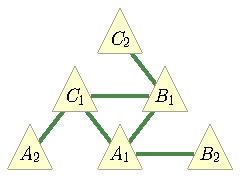
\includegraphics[scale=1]{injectiongraph222.pdf}
\caption{The injection graph corresponding to the inflated DAG in \cref{fig:Tri222}, wherein a pair of nodes are adjacent iff they are pairwise injectable.}\label{fig:injection222}
\end{minipage}
\hfill
\begin{minipage}[t]{0.3\linewidth}
\centering
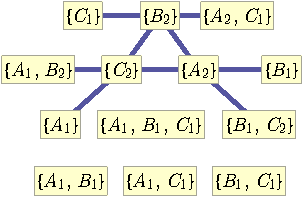
\includegraphics[scale=1]{preinjectiongraph222.pdf}
\caption{The pre-injection graph corresponding to the inflated DAG in \cref{fig:Tri222}, wherein a pair of injectable sets are adjacent iff they are ancestrally independent. }\label{fig:preinjectiongraph222}
\end{minipage}
\hfill
\begin{minipage}[t]{0.3\linewidth}
\centering
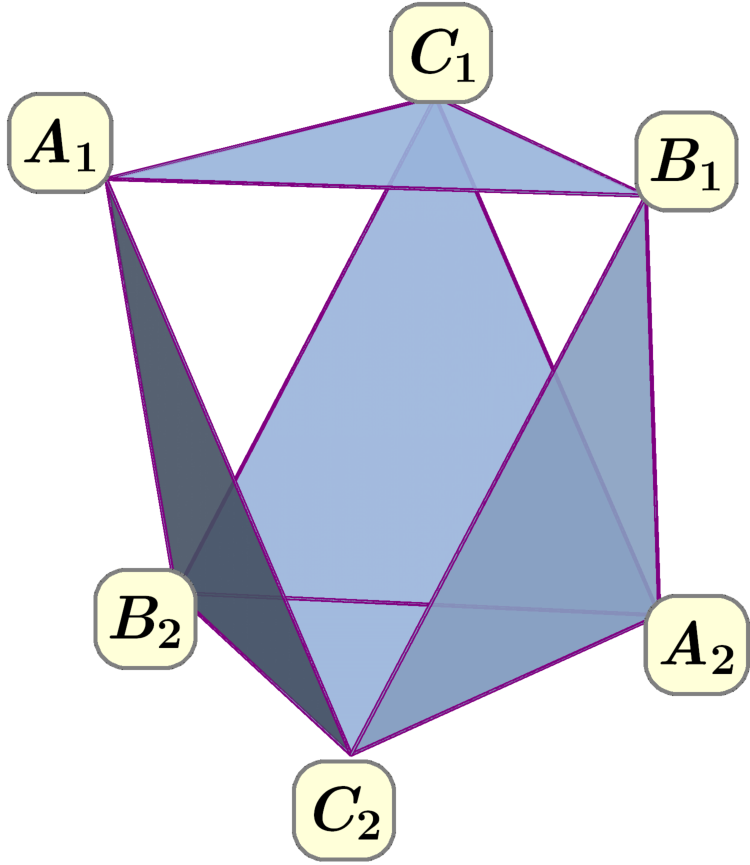
\includegraphics[scale=0.25]{simplicialcomplex.pdf}
\caption{The simplicial complex of pre-injectable sets for the inflation of~\cref{fig:Tri222}. The 5 faces correspond to the maximal pre-injectable sets, namely $\{A_1 B_1 C_1\}$, $\{A_1 B_2 C_2\}$, $\{A_2 B_1 C_2\}$, $\{A_2 B_2 C_1\}$ and $\{A_2 B_2 C_2\}$.}\label{fig:simplicialcomplex222}
\end{minipage}
\end{figure}

%\begin{figure}[t]
%\centering
%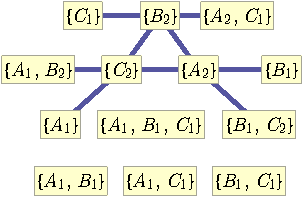
\includegraphics[scale=1]{preinjectiongraph222.pdf}
%\caption{***Pre-injection graph}\label{fig:preinjectiongraph222}
%\end{figure}

From \cref{fig:injection222,fig:preinjectiongraph222}, we easily infer the injectable sets and the maximal pre-injectable sets, as well as the partition of the maximal pre-injectable sets into ancestrally independent subsets, for the inflated DAG of \cref{fig:Tri222} to be:
\begin{align}\label{eq:basicsetup222}
%{\underbrace{\begin{matrix}
%A_2\aindep B_1\\
%A_2\aindep C_2\\
%B_2\aindep A_2\\
%B_2\aindep C_1\\
%C_2\aindep A_1\\
%C_2\aindep B_2
%\end{matrix}}_{\substack{\text{ancestrally independent}\\\text{pairs of nodes}}}}
%\qquad\qquad
{\underbrace{\begin{matrix}
\, \\
\brackets{A_1},\:\brackets{B_1},\:\brackets{C_1},\\
\brackets{A_2},\:\brackets{B_2},\:\brackets{C_2},\\
\brackets{A_1 B_1},\:\brackets{A_1 C_1},\:\brackets{B_1 C_1},\\
\brackets{A_1 B_2}.\:\brackets{A_2 C_1},\:\brackets{B_1 C_2},\\
\brackets{A_1 B_1 C_1}
\end{matrix}}_{\substack{\text{injectable sets}}}}
%\qquad\quad
%{\underbrace{\begin{matrix}
%\\ \\
%\brackets{A_2}\aindep \brackets{B_1 B_2 C_2}\\
%\brackets{B_2}\aindep \brackets{A_2 C_1 C_2}\\
%\brackets{C_2}\aindep \brackets{A_1 A_2 B_2}\\
%\brackets{A_2}\aindep \brackets{B_2}\aindep \brackets{C_2}
%\end{matrix}}_{\substack{\text{maximal}\\\text{ancestral}\\\text{independencies}}}}
%\qquad\quad
%{\underbrace{\begin{matrix}
%\brackets{ A_1 B_1 }\\
%\brackets{ B_1 C_1 }\\
%\brackets{ A_1 C_1 }\\
%\brackets{ A_2 C_1 }\\
%\brackets{ B_2 A_1 }\\
%\brackets{ C_2 B_1 }\\
%\end{matrix}}_{\substack{\text{pairwise}\\\text{injectable}\\\text{sets}}}}
\qquad\qquad
{\underbrace{\begin{matrix}
\brackets{A_1 B_1 C_1} \\
\brackets{A_1 B_2 C_2} \\
\brackets{B_1 C_2 A_2} \\
\brackets{C_1 A_2 B_2} \\
\brackets{A_2 B_2 C_2}
\end{matrix}}_{\substack{\text{maximal}\\\text{pre-injectable sets}}}}
\qquad
{\underbrace{\begin{matrix}
\\
\{A_1 B_2\} \aindep \{ C_2\} \\
\{B_1 C_2\} \aindep \{ A_2\} \\
\{C_1 A_2\} \aindep \{ B_2\} \\
\{A_2\} \aindep \{B_2\} \aindep \{ C_2\}
\end{matrix}}_{\substack{\text{relevant}\\\text{ancestral independences}}}}
\end{align}
%where we have placed commas in the maximal pre-injectable sets in order to indicate how each of these arises as a disjoint union of injectable sets with disjoint ancestry, which one can read off from the corresponding clique in the independence graph. 
Using the ancestral independence relations, the marginal distributions for the maximal pre-injectable sets factorize in the manner described by the right-hand side of \cref{eq:tri222fac}.
%This results in the distributions on the pre-injectable sets being given in terms of distribution on the original DAG via
%\begin{align}\label{eq:preinjectableuses222}
%\begin{split}
%&\forall{a b c}:\; \begin{cases}
%\pdf[A_1 B_1 C_1]{a b c} = \pdf[A B C]{a b c} \\
%\pdf[A_1 B_2 C_2]{a b c} = \pdf[C]{c}\pdf[A B]{a b}\\%\pdf{C}\pdf{A B}\\
%\pdf[A_2 B_1 C_2]{a b c} = \pdf[A]{a}\pdf[B C]{b c}\\
%\pdf[A_2 B_2 C_1]{a b c} = \pdf[B]{b}\pdf[A C]{a c}\\
%\pdf[A_2 B_2 C_2]{a b c} = \pdf[A]{a}\pdf[B]{b}\pdf[C]{c}
%\end{cases}\end{split}
%\end{align}
%\cref{eq:preinjectableuses222} is an equivalent restatement of \cref{eq:tri222fac}. 
%Having identified the pre-injectable sets (and how to use them), we next consider various ways to invoke constraints on the distributions over the pre-injectable sets.

Having identified the pre-injectable sets together with the factorization relations implied by ancestral independences, we now discuss how to obtain constraints on the marginal distributions over the pre-injectable sets.

\subsection{The marginal problem}\label{step:marginalsproblem}
%\subsection{Constraining distributions over the pre-injectable sets via the marginal problem}

For a given family of marginal distributions, each defined on a subset of the variables, determining whether there exists a joint probability distribution over the full set of variables from which all of these can be obtained as marginal distributions is known as the {\em marginal problem}.
%they can be obtained through marginalization of a single joint probability 
%The most trivial constraint on possible marginal probabilities, regardless of causal structure,  
%on the pre-injectable set
%is simply the \emph{existence of some joint probability distribution} from which the marginal distributions can be recovered through marginalization. 
%This isn't really causal inference---as no nontrivial causal hypothesis is considered---but rather more of a preliminary sanity check. If the marginal distributions are not \tblue{consistent}, then the answer to ``Can these marginal distributions be explained by this particular causal hypothesis?'' is automatically ``No''. 
%This type of problem is known as a \tblue{marginal problem}. 
For some of its history and for further references, see~\cite{fritz2013marginal}; for a more modern account using the language of presheaves, see~\cite{abramsky_contextuality_2011}.

%More precisely, a \emph{marginal problem} is specified by 
To specify such a problem, one must specify the full set of variables to be considered, denoted $\bm{X}$, together with a family of subsets of $\bm{X}$, denoted $(\bm{U}_1,\ldots,\bm{U}_n)$ and called \tblue{contexts}.
%, as well as a specification of the (finite) number of outcomes that each variable is allowed to take. 
A family of contexts can be visualized through 
%It may help to draw the visualize contexts in terms of 
the simplicial complex that they generate, as the example in~\cref{fig:simplicialcomplex222} illustrates. Every joint distribution $P_{\bm{X}}$ %marginalization to each of $(\bm{U}_1,\ldots,\bm{U}_n)$, 
defines a family of marginal distributions, $(P_{\bm{U}_1},\ldots,P_{\bm{U}_n})$ through marginalization,  $P_{\bm{U}_i} := \sum_{\bm{X} \setminus \bm{U}_i} P_{\bm{X}}$. A \emph{marginal problem} concerns the converse inference.  A family of distributions $(P_{\bm{U}_1},\ldots,P_{\bm{U}_n})$ is given, and one wants to find conditions for when a joint distribution $\hat{P}_{\bm{X}}$ exists which reproduces given marginals, $P_{\bm{U}_i} = \sum_{\bm{X}\setminus\bm{U}_i} \hat{P}_{\bm{X}}$ for all $i$.
%as $P_{\bm{U}_i} = \hat{P}_{\bm{U}_i}$ for all $i$?

There is a simple necessary condition: in order for $\hat{P}_{\bm{X}}$ to exist, the marginals clearly must be consistent, in the sense that marginalizing $P_{\bm{U}_i}$ to the variables in $\bm{U}_i\cap\bm{U}_j$ results in the same distribution as marginalizing $P_{\bm{U}_j}$ to those variables.  
%\footnote{This is difficult to express explicitly in our notation, since $P_{\bm{U}_i\cap \bm{U}_j}$ could refer to either marginal.}. 
 %we have already seen in the previous section, 
 In many cases this is not sufficient; indeed, we have already seen examples of additional constraints, namely, the inequalities \eqref{eq:polymonogamyraw}, \eqref{eq:MIraw} and \eqref{eq:FritzF3raw} from Sec.~\ref{Sec:DerivingInequalities}\footnote{Depending on how the contexts intersect with one another, this \emph{may} be sufficient. A precise characterization for when this occurs has been found by~\citet{vorobev_extension_1960}.}. So what are the necessary and sufficient conditions?

To answer this question, it helps to realize two things:
\begin{itemize}
	\item The set of possibilities for the distribution $P_{\bm{X}}$ is the convex hull of the deterministic assignments of values to $\bm{X}$ (the point distributions), and 
%	Every joint distribution $P_{\bm{X}}$ is a convex combination of deterministic assignments of values to all variables (delta distributions), and conversely.
	\item The map $P_{\bm{X}}\to (P_{\bm{U}_1},\ldots,P_{\bm{U}_n})$, describing marginalization to each of the contexts in $(\bm{U}_1,\ldots,\bm{U}_n)$, is linear.
\end{itemize}
Hence the image of the set of possibilities for the distribution $P_{\bm{X}}$ under the map $P_{\bm{X}}\to (P_{\bm{U}_1},\ldots,P_{\bm{U}_n})$ is exactly the convex hull of the deterministic assignments of values to $(\bm{U}_1,\ldots,\bm{U}_n)$ (more precisely, the deterministic assignments that are consistent where these contexts overlap). Since there are only finitely many such deterministic assignments, this convex hull is a polytope; it is called the \tblue{marginal polytope}~\cite{kahle_marginal_2010}. Together with the above equations on coinciding submarginals, the facet inequalities of the marginal polytope form necessary and sufficient conditions for the marginal problem to have a solution.

%Thus solving the marginal problem is an instance of a facet enumeration problem, or equivalently a linear quantifier elimination problem;~\cref{sec:projalgorithms} gives an overview of how to solve this in practice. 


% quantifier-free form in terms of inequalities such that satisfaction of all such inequalities is necessary and sufficient for marginal compatibility. An efficient algorithm to solve the marginal problem is given in \cref{sec:projalgorithms}. The marginal problem comes up in a variety of applications, and has been studied extensively; see~\cite{fritz2013marginal} for further references.

As every facet enumeration problem, this can also be phrased as a problem of \tblue{linear quantifier elimination}. We illustrate this with the example of the marginal problem where $\bm{X} := \{ A_1, A_2, B_1, B_2, C_1, C_2\}$ and the contexts are the 
%case of the five three-variable marginal distributions corresponding to the 
maximal pre-injectable sets in \cref{eq:basicsetup222}.
% For simplicity, we assume that all observable variables are binary.
%\footnote{If the observables are not binary, then the resulting  binary-outcome inequalities are necessary for marginal compatibility, in that they should hold for any course-graining of the observational data into two classes, but the binary-outcome inequalities are no longer sufficient.}.
% In order for the five pre-injectable sets in \cref{eq:preinjectableuses222} to be marginally compatible there must exist 64 nonnegative joint probabilities, i.e. satisfying
Besides normalization of probability, the only constraint on the probabilities making up the joint distribution is nonnegativity,
\begin{align}\label{eq:nonnegativity}
\forall{a_1 a_2 b_1 b_2 c_1 c_2}:\; \pdf[A_1 A_2 B_1 B_2 C_1 C_2]{a_1 a_2 b_1 b_2 c_1 c_2} \geq 0.
\end{align}
We require the joint distribution to reproduce the marginal distribution on each context via
\begin{align}\label[eqs]{eq:marginalequalities222}
\begin{split}
&\forall{a_1 b_1 c_1}:\;\pdf[A_1 B_1 C_1]{a_1 b_1 c_1} = \sum\nolimits_{a_2 b_2 b_2}\pdf[A_1 A_2 B_1 B_2 C_1 C_2]{a_1 a_2 b_1 b_2 c_1 c_2},\\
&\forall{a_1 b_2 c_2}:\;\pdf[A_1 B_2 C_2]{a_1 b_2 c_2} = \sum\nolimits_{a_2 b_1 c_1}\pdf[A_1 A_2 B_1 B_2 C_1 C_2]{a_1 a_2 b_1 b_2 c_1 c_2},\\
&\forall{a_2 b_1 c_2}:\;\pdf[A_2 B_1 C_2]{a_2 b_1 c_2} = \sum\nolimits_{a_1 b_2 c_1}\pdf[A_1 A_2 B_1 B_2 C_1 C_2]{a_1 a_2 b_1 b_2 c_1 c_2},\\
&\forall{a_2 b_2 c_1}:\;\pdf[A_2 B_2 C_1]{a_2 b_2 c_1} = \sum\nolimits_{a_1 b_1 c_2}\pdf[A_1 A_2 B_1 B_2 C_1 C_2]{a_1 a_2 b_1 b_2 c_1 c_2},\\
&\forall{a_2 b_2 c_2}:\;\pdf[A_2 B_2 C_2]{a_2 b_2 c_2} = \sum\nolimits_{a_1 b_1 c_1}\pdf[A_1 A_2 B_1 B_2 C_1 C_2]{a_1 a_2 b_1 b_2 c_1 c_2}.
\end{split}
\end{align}
%For example in the case of binary variables, we therefore 
If each variable is binary, then we have $64$ inequalities and $40$ equations, although the latter are not all independent. 

The marginal problem is a linear system of equations and inequalities relating the unknown joint probabilities to the accessible marginal probabilities. The problem of quantifier elimination consists in finding an equivalent system of equations and inequalities that is satisfied if and only if the original system has a solution for the unknown probabilities. This requires eliminating 64 unknowns $\p[A_1 A_2 B_1 B_2 C_1 C_2]{a_1 a_2 b_1 b_2 c_1 c_2}$ for each of the 64 choices of the values $a_1,\ldots,c_2$. The resulting new system consists of the coinciding-submarginals equations together with the facet inequalities of the marginal polytope.
%joint probabilities $\{ \p[A_1 A_2 B_1 B_2 C_1 C_2]{a_1 a_2 b_1 b_2 c_1 c_2} : (a_1 a_2 b_1 b_2 c_1 c_2) {\underline{\phantom{xxxxx}}}$, 
%and to thereby compute the inequalities that constrain the marginal probabilities.
%We coin the term gedankenprobability to denote any probability pertaining to a \emph{not}-pre-injectable set of inflation-DAG variables. The gedankenprobabilities evoke thought experiments, because any \purp{black box implementation of the original causal structure % \emph{in-principle}.

It is helpful to formalize the marginal problem in terms of a \tblue{marginal description matrix} $\mblue{\bm{M}}$, a \tblue{marginal distribution vector} $\mblue{\bm{b}}$, and some unknown \tblue{joint distribution vector} $\mblue{\bm{x}}$. The marginal problem can the be stated as
\begin{align}\label{eq:marginalproblemgeneric}
    \exists_{\bm{x} \bm{\geq} \bm{0}} \text{ s.t. }\bm{M}.\bm{x}\bm{=}\bm{b}
\end{align}
where in the example we have been discussing $\bm{M}$ would be a $48\times 64$ matrix, such that $\bm{M}.\bm{x}\bm{=}\bm{b}$ represents 48 equations and $\bm{x} \bm{\geq} \bm{0}$ represents 64 inequalities. Note that the marginal description matrix $\bm{M}$ only has zeroes and ones as its constituent elements.

Linear quantifier elimination is already used in causal inference for deriving entropic causal compatibility inequalities \cite{chaves2014novel,chaves2014informationinference}. In that task, however, the unknowns being eliminated are entropies on sets of variables of which one or more is latent. By contrast, the unknowns being eliminated above are all probabilities on sets of variables all of which are observed---but on the inflated DAG rather than the original DAG.
%The unknowns we eliminate are the not-pre-injectable joint probabilities, which are, at least on first look, quite different from probabilities involving latent variables;
\cref{sec:Bellscenarios} will partly elucidate the relation.

The marginal problem is a standard facet enumeration problem, in that the vertices of the polytope are given. The derivation of entropic inequalities, by contrast, is a priori only a linear quantifier elimination task, and more difficult to cast as a facet enumeration problem with given vertices, since the vertices (extremal rays) of the Shannon cone elude a simple description. As such, while facet enumeration tools are useful for deriving polynomial inequalities via the inflation technique, they are not directly available for the derivation of entropic inequalities; see \cref{sec:projalgorithms} for further details.

\subsection{Witnessing incompatibility by non-sastisfiability of the marginal problem}\label{sec:satisfiable}

Given a particular distribution of observable nodes of the original DAG, one can use the inflation technique to probe causal compatibility as follows. Using \cref{mainlemma} along with the factorization conditions implied by ancestral independences among the variables in the maximal pre-injectable sets, one can infer the distributions on the maximal pre-injectable sets pursuant to the given original-scenario distribution; this was the first step in each example in \cref{subsec:witnessingincompat}. This amounts to having known numerical values for %the left-hand sides of the equations defining the marginal problem, such as \cref{eq:marginalequalities222}. 
the marginal distribution vector, $\bm{b}\to\bm{b}_{\mbox{numeric}}$ in \cref{eq:marginalproblemgeneric}. A single linear program can then assess whether the marginal problem equalities can be solved using nonnegative values for the unknown joint probabilities or not. If the marginal problem cannot be satisfied, then the original distribution is witnessed as incompatible with the original DAG. 

As this satisfiability problem is a linear program, testing specific distributions for causal compatibility for a given inflation DAG is computationally inexpensive. For instance, using the rather complex inflation of the Triangle scenario depicted in \cref{fig:TriFullDouble}, our numerical computations have reproduced~\cite[Theorem~2.16]{fritz2012bell}: a certain distribution, inspired by Bell's theorem, is incompatible with the Triangle scenario despite being realizable on the Triangle DAG with quantum systems on the latent nodes.

When $\bm{M}.\bm{x}\bm{=}\bm{b}_{\text{numeric}}$ has no positive solution $\bm{x}$ then the system is considered \tblue{primal infeasible}. Many linear programming tools are capable of returning a \tblue{Farkas infeasibility certificate} \cite{infeasibilitycertificates} whenever a linear system is primal infeasible\footnote{Farkas infeasibility certificates are available, for example, in \href[pdfnewwindow]{http://docs.mosek.com/8.0/pythonapi/optimizer-task-gety.html}{\textit{Mosek}}, \href[pdfnewwindow]{https://www.gurobi.com/documentation/6.5/refman/farkasdual.html}{\textit{Gurobi}}, and \href[pdfnewwindow]{http://www-01.ibm.com/support/docview.wss?uid=swg21400058}{\textit{CPLEX}}, as well as by accessing dual variables in \href[pdfnewwindow]{http://cvxr.com/cvx/doc/basics.html\#dual-variables}{\textit{cvxr}}/\href[pdfnewwindow]{http://cvxopt.org/userguide/coneprog.html\#linear-cone-programs}{\textit{cvxopt}}.}. The infeasibility certificate is a vector $\bm{y}$ of the same length as  $\bm{b}_{\text{numeric}}$ which can be used to generate the (scalar) marginal-consistency inequality  $\bm{y}.\bm{b}\geq 0$ which is violated for $\bm{b}\to\bm{b}_{\text{numeric}}$. One can readily verify that the infeasibility certificate $\bm{y}$ maps the marginal description matrix $\bm{M}$ to some nonnegtive vector; that is to say $\bm{y}.\bm{M}\bm{\geq} \bm{0}$ so therefore 
\begin{align}\label{eq:certificateproof}
    \exists_{\bm{x} \bm{\geq} \bm{0}} \text{ s.t. } \bm{y}.\bm{M}.\bm{x}=\bm{y}.\bm{b} \quad\implies\quad \bm{y}.\bm{b}\geq 0
\end{align}

\subsection{Causal compatibility inequalities via a complete solution of the marginal problem}\label{sec:CCineqs}

For deriving causal compatibility inequalities systematically, one chooses an inflation DAG and identifies the maximal pre-injectable sets as per the above. Then ones solves the marginal problem via facet enumeration\footnote{In \cref{sec:projalgorithms}, we provide an overview of techniques for facet enumeration.} of the marginal polytope, where the contexts are the maximal pre-injectable sets. This results in linear inequalities at the level of the inflation DAG.
%As we note there, it can be reduced to a linear quantifier elimination problem, which is the technique we apply here.
By substituting into these inequalities the factorization conditions implied by ancestral independences per \cref{eq:preinjfactor}, one obtains causal compatibility inequalities for the inflated DAG.  Finally, these can be converted into causal compatibility inequalities for the original DAG using \cref{maincorollary}.

%\color{purple} Move this paragraph to later. \color{black}
%Given a facet of the marginal polytope---or any other linear inequality that bounds it---we can construct a polynomial inequality for our original causal inference problem by plugging in the factorization relations of \cref{mainlemma}. Doing the same with the equations of coinciding submarginals shows that these are trivially satisfied, and thus it is only the inequalities that are of interest to us.



As an example, 
%To illustrate the power of the inflation technique, 
we present all of the causal compatibility inequalities that one can derive for the Triangle scenario with binary observed variables using the inflation of \cref{fig:Tri222}. The contexts for the marginal problem are the maximal pre-injectable sets of \cref{eq:basicsetup222} and \cref{fig:simplicialcomplex222}, and we solve the latter using facet enumeration. It turns out that the marginal polytope has 64 symmetry classes of facets, where the symmetry transformations are given by permutations of the observed variables, flipping the value of one variable, and composites of these.
%The following polynomial inequalities for the Triangle scenario with binary observed variables have been derived via the linear quantifier elimination method of~\cref{sec:ineqs} using the inflated DAG of~\cref{fig:Tri222}. 
%This results in 64 symmetry classes of causal compatibility inequalities for the Triangle scenario, where the symmetries are given by permuting the variables and inverting the outcomes. 
Applying the factorization of probabilities according to ancestral independences per \cref{eq:basicsetup222} and converting into inequalities for the original DAG using \cref{maincorollary} results in 64 polynomial inequalities up to symmetry. However, there is no guarantee that each one of these inequalities is nontrivial at the level of the original DAG, where nontriviality of an inequality means that it is violated by at least one distribution. Numerically, we find that only 37 of these inequalities are nontrivial. We present them here\footnote{A machine-readable version of this list of inequalities may be found in \cref{sec:38ineqs}.} in correlator form:
 %For the resulting 64 inequalities, numerical checks have found violations of only 38 of them: although they are all facets of the marginal polytope over the distributions on pre-injectable sets, there is no guarantee that they are also nontrivial inequalities at the level of the original DAG, and this has indeed turned out not to be the case for 26 of these symmetry classes of inequalities. 
\begin{align*}%\label{nontriv.humanreadable}
\hspace{-\mathindent}\resizebox{\linewidth}{!}{\(
\begin{array}{ll}
 \text{($\#$} 1^* \text{):  } & 0\leq 1+\expec{B} \expec{C}+\expec{AB}+\expec{AC} \\
 \text{($\#$} 2 \text{):  } & 0\leq 2+\expec{A} \expec{B} \expec{C}-\expec{C} \expec{AB}-2 \expec{AC} \\
 \text{($\#$} 3^* \text{):  } & 0\leq 3+\expec{A}-\expec{B}+\expec{C}+\expec{B} \expec{C}+\expec{A} \expec{B}
   \expec{C}+\expec{AB}-\expec{C} \expec{AB}+3 \expec{AC}-\expec{B} \expec{AC} \\
 \text{($\#$} 4^* \text{):  } & 0\leq 3+\expec{A}-\expec{B}+\expec{C}+\expec{B} \expec{C}-\expec{A} \expec{B}
   \expec{C}+\expec{AB}+\expec{C} \expec{AB}+3 \expec{AC}-\expec{B} \expec{AC} \\
 \text{($\#$} 5 \text{):  } & 0\leq 3+\expec{B}-\expec{A} \expec{B}+\expec{A} \expec{C}+\expec{A} \expec{B}
   \expec{C}+\expec{AB}+\expec{C} \expec{AB}-\expec{B} \expec{AC}-2 \expec{BC} \\
 \text{($\#$} 6 \text{):  } & 0\leq 3+\expec{B}+\expec{A} \expec{C}+\expec{A} \expec{B} \expec{C}-\expec{C} \expec{AB}-2
   \expec{AC}-\expec{B} \expec{AC}-2 \expec{BC} \\
 \text{($\#$} 7 \text{):  } & 0\leq 3+\expec{B}+\expec{A} \expec{B}-\expec{A} \expec{C}-\expec{A} \expec{B}
   \expec{C}+\expec{AB}+\expec{C} \expec{AB}+\expec{B} \expec{AC}-2 \expec{BC} \\
 \text{($\#$} 8^* \text{):  } & 0\leq 3+\expec{A}+\expec{B}+\expec{A} \expec{B}+\expec{C}+\expec{A} \expec{C}+\expec{B}
   \expec{C}-\expec{A} \expec{B} \expec{C}+2 \expec{AB}+\expec{C} \expec{AB}+2 \expec{AC}+\expec{B} \expec{AC}+2 \expec{BC}+\expec{A}
   \expec{BC}-\expec{ABC} \\
 \text{($\#$} 9^* \text{):  } & 0\leq 3+\expec{A}+\expec{B}-\expec{A} \expec{B}+\expec{C}+\expec{A} \expec{C}+\expec{B}
   \expec{C}-\expec{A} \expec{B} \expec{C}+\expec{C} \expec{AB}+2 \expec{AC}+\expec{B} \expec{AC}-2 \expec{BC}-\expec{A}
   \expec{BC}+\expec{ABC} \\
 \text{($\#$} 10^* \text{):  } & 0\leq 4+2 \expec{A} \expec{B}+2 \expec{C}+2 \expec{B} \expec{C}-2 \expec{AB}+\expec{C} \expec{AB}-2
   \expec{AC}+\expec{B} \expec{AC}+\expec{A} \expec{BC}-\expec{ABC} \\
 \text{($\#$} 11^* \text{):  } & 0\leq 4-2 \expec{B}+\expec{B} \expec{C}+\expec{A} \expec{B} \expec{C}-2 \expec{AB}+\expec{C}
   \expec{AB}-\expec{B} \expec{AC}-3 \expec{BC}+\expec{ABC} \\
 \text{($\#$} 12^* \text{):  } & 0\leq 4-2 \expec{B}+2 \expec{A} \expec{C}+\expec{B} \expec{C}-\expec{A} \expec{B} \expec{C}-2
   \expec{AB}+\expec{C} \expec{AB}-2 \expec{AC}+\expec{B} \expec{AC}-3 \expec{BC}+\expec{ABC} \\
 \text{($\#$} 13^* \text{):  } & 0\leq 4-2 \expec{A} \expec{B}-2 \expec{A} \expec{C}-\expec{B} \expec{C}-\expec{A} \expec{B}
   \expec{C}+2 \expec{AB}-\expec{C} \expec{AB}-2 \expec{AC}+\expec{B} \expec{AC}+\expec{BC}+\expec{ABC} \\
 \text{($\#$} 14^* \text{):  } & 0\leq 4-2 \expec{A} \expec{B}+2 \expec{A} \expec{C}-\expec{B} \expec{C}+\expec{A} \expec{B}
   \expec{C}+2 \expec{AB}+\expec{C} \expec{AB}-2 \expec{AC}+\expec{B} \expec{AC}+\expec{BC}+\expec{ABC} \\
 \text{($\#$} 15^* \text{):  } & 0\leq 4+2 \expec{A} \expec{C}+\expec{B} \expec{C}+\expec{A} \expec{B} \expec{C}-\expec{C} \expec{AB}-2
   \expec{AC}-\expec{B} \expec{AC}+3 \expec{BC}+\expec{ABC} \\
 \text{($\#$} 16^* \text{):  } & 0\leq 4-2 \expec{B}+2 \expec{A} \expec{C}-2 \expec{AB}+\expec{C} \expec{AB}-2 \expec{AC}+\expec{B}
   \expec{AC}-2 \expec{BC}-\expec{A} \expec{BC}+\expec{ABC} \\
 \text{($\#$} 17^* \text{):  } & 0\leq 4+2 \expec{A} \expec{B}+2 \expec{A} \expec{C}+2 \expec{B} \expec{C}-2 \expec{AB}+\expec{C}
   \expec{AB}-2 \expec{AC}+\expec{B} \expec{AC}-2 \expec{BC}+\expec{A} \expec{BC}+\expec{ABC} \\
 \text{($\#$} 18 \text{):  } & 0\leq 5+\expec{A}+\expec{B}-2 \expec{A} \expec{B}+\expec{C}+\expec{B} \expec{C}+\expec{A} \expec{B}
   \expec{C}+3 \expec{AB}+\expec{C} \expec{AB}+\expec{AC}-\expec{B} \expec{AC}-4 \expec{BC} \\
 \text{($\#$} 19^* \text{):  } & 0\leq 5+\expec{A}+\expec{B}+2 \expec{A} \expec{B}+\expec{C}-2 \expec{A} \expec{C}+\expec{B}
   \expec{C}-\expec{A} \expec{B} \expec{C}+3 \expec{AB}+\expec{C} \expec{AB}-\expec{AC}+\expec{B} \expec{AC}-4 \expec{BC} \\
 \text{($\#$} 20^* \text{):  } & 0\leq 5+\expec{A}-\expec{B}-2 \expec{A} \expec{B}+\expec{C}-\expec{A} \expec{C}+\expec{B}
   \expec{C}+\expec{AB}+\expec{C} \expec{AB}+2 \expec{AC}-2 \expec{B} \expec{AC}-2 \expec{BC}-2 \expec{A} \expec{BC}-2 \expec{ABC} \\
 \text{($\#$} 21^* \text{):  } & 0\leq 5+\expec{A}+\expec{B}+\expec{C}-\expec{A} \expec{C}-\expec{B} \expec{C}-2 \expec{A} \expec{B}
   \expec{C}+\expec{AB}+2 \expec{C} \expec{AB}+2 \expec{AC}+\expec{B} \expec{AC}-2 \expec{BC}+\expec{A} \expec{BC}-\expec{ABC} \\
 \text{($\#$} 22^* \text{):  } & 0\leq 5-\expec{A}+\expec{B}-2 \expec{A} \expec{B}+\expec{C}-2 \expec{A} \expec{C}+2 \expec{B}
   \expec{C}+\expec{AB}-2 \expec{C} \expec{AB}+\expec{AC}-2 \expec{B} \expec{AC}-\expec{BC}-2 \expec{A} \expec{BC}+\expec{ABC} \\
 \text{($\#$} 23^* \text{):  } & 0\leq 5+\expec{A}+\expec{B}-\expec{A} \expec{B}+\expec{C}+2 \expec{B} \expec{C}+\expec{A} \expec{B}
   \expec{C}+2 \expec{AB}-\expec{C} \expec{AB}+\expec{AC}-2 \expec{B} \expec{AC}-\expec{BC}-2 \expec{A} \expec{BC}+\expec{ABC} \\
 \text{($\#$} 24^* \text{):  } & 0\leq 5+\expec{A}+\expec{B}-2 \expec{A} \expec{B}+\expec{C}-\expec{A} \expec{C}-\expec{B} \expec{C}-2
   \expec{A} \expec{B} \expec{C}-\expec{AB}+2 \expec{C} \expec{AB}+2 \expec{AC}+\expec{B} \expec{AC}+2 \expec{BC}-\expec{A}
   \expec{BC}+\expec{ABC} \\
 \text{($\#$} 25 \text{):  } & 0\leq 6+2 \expec{A} \expec{B}+\expec{A} \expec{C}+2 \expec{B} \expec{C}+\expec{A} \expec{B} \expec{C}-4
   \expec{AB}-2 \expec{C} \expec{AB}-3 \expec{AC}-\expec{B} \expec{AC}-2 \expec{A} \expec{BC} \\
 \text{($\#$} 26 \text{):  } & 0\leq 6-2 \expec{A}+\expec{A} \expec{B}+2 \expec{C}+\expec{A} \expec{C}+2 \expec{A} \expec{B}
   \expec{C}-5 \expec{AB}-\expec{C} \expec{AB}-3 \expec{AC}+\expec{B} \expec{AC}-2 \expec{A} \expec{BC} \\
 \text{($\#$} 27 \text{):  } & 0\leq 6+2 \expec{A} \expec{B}+2 \expec{C}+\expec{A} \expec{C}+\expec{A} \expec{B} \expec{C}-4
   \expec{AB}-2 \expec{C} \expec{AB}+3 \expec{AC}+\expec{B} \expec{AC}-2 \expec{A} \expec{BC} \\
 \text{($\#$} 28 \text{):  } & 0\leq 6+\expec{A} \expec{B}+\expec{A} \expec{C}-4 \expec{B} \expec{C}-2 \expec{A} \expec{B}
   \expec{C}+\expec{AB}+\expec{C} \expec{AB}-3 \expec{AC}-\expec{B} \expec{AC}+2 \expec{BC}-2 \expec{A} \expec{BC} \\
 \text{($\#$} 29 \text{):  } & 0\leq 6+2 \expec{B}+\expec{A} \expec{B}-2 \expec{A} \expec{C}+\expec{B} \expec{C}-2 \expec{A} \expec{B}
   \expec{C}+3 \expec{AB}+\expec{C} \expec{AB}+2 \expec{B} \expec{AC}-5 \expec{BC}+\expec{A} \expec{BC} \\
 \text{($\#$} 30 \text{):  } & 0\leq 6+2 \expec{B}-2 \expec{A} \expec{B}+4 \expec{A} \expec{C}-\expec{B} \expec{C}+\expec{A} \expec{B}
   \expec{C}+2 \expec{AB}+2 \expec{C} \expec{AB}-2 \expec{AC}+2 \expec{B} \expec{AC}+\expec{BC}+\expec{A} \expec{BC} \\
 \text{($\#$} 31 \text{):  } & 0\leq 6+\expec{A} \expec{C}+4 \expec{B} \expec{C}+\expec{A} \expec{B} \expec{C}-2 \expec{AB}-2 \expec{C}
   \expec{AB}-3 \expec{AC}-\expec{B} \expec{AC}-2 \expec{BC}-2 \expec{ABC} \\
 \text{($\#$} 32 \text{):  } & 0\leq 7+\expec{A}+\expec{B}+\expec{A} \expec{B}+\expec{C}-2 \expec{A} \expec{C}+2 \expec{B}
   \expec{C}-\expec{A} \expec{B} \expec{C}+2 \expec{AB}+3 \expec{C} \expec{AB}+\expec{AC}+2 \expec{B} \expec{AC}-3 \expec{BC}-2
   \expec{A} \expec{BC}+3 \expec{ABC} \\
 \text{($\#$} 33 \text{):  } & 0\leq 8+2 \expec{A} \expec{B}+4 \expec{A} \expec{C}-2 \expec{B} \expec{C}+2 \expec{A} \expec{B}
   \expec{C}-2 \expec{AB}-\expec{C} \expec{AB}-4 \expec{AC}+\expec{B} \expec{AC}-2 \expec{BC}-3 \expec{A} \expec{BC}-3 \expec{ABC} \\
 \text{($\#$} 34 \text{):  } & 0\leq 8+2 \expec{A}-2 \expec{C}-\expec{A} \expec{C}+2 \expec{B} \expec{C}+3 \expec{A} \expec{B}
   \expec{C}-6 \expec{AB}+\expec{C} \expec{AB}+\expec{AC}+2 \expec{B} \expec{AC}-3 \expec{A} \expec{BC}+\expec{ABC} \\
 \text{($\#$} 35 \text{):  } & 0\leq 8+2 \expec{A}+\expec{A} \expec{C}+2 \expec{B} \expec{C}+3 \expec{A} \expec{B} \expec{C}+6
   \expec{AB}-\expec{C} \expec{AB}+\expec{AC}-2 \expec{B} \expec{AC}-2 \expec{BC}-3 \expec{A} \expec{BC}+\expec{ABC} \\
 \text{($\#$} 36 \text{):  } & 0\leq 8-2 \expec{B}+2 \expec{A} \expec{B}-2 \expec{C}-\expec{B} \expec{C}-3 \expec{A} \expec{B}
   \expec{C}+3 \expec{C} \expec{AB}-6 \expec{AC}+\expec{B} \expec{AC}+\expec{BC}-2 \expec{A} \expec{BC}+\expec{ABC} \\
 \text{($\#$} 37 \text{):  } & 0\leq 8+2 \expec{B}+\expec{A} \expec{B}-2 \expec{A} \expec{C}-3 \expec{A} \expec{B}
   \expec{C}+\expec{AB}+2 \expec{C} \expec{AB}+2 \expec{AC}+3 \expec{B} \expec{AC}-6 \expec{BC}-\expec{A} \expec{BC}+\expec{ABC} \\
\end{array}
\)}
\end{align*}
Moreover, it is likely to be the case that these 37 symmetry classes of causal compatibility inequalities are not a minimal generating set, where a minimal generating set is defined to be one such that, for every inequality, there is a distribution that violates it while satisfying all of the others. 
%; we have not yet checked whether for every inequality there is a distribution which violates that inequality but satisfies all the others.
%
%\clearpage
%\label{page:nontrivlist}
%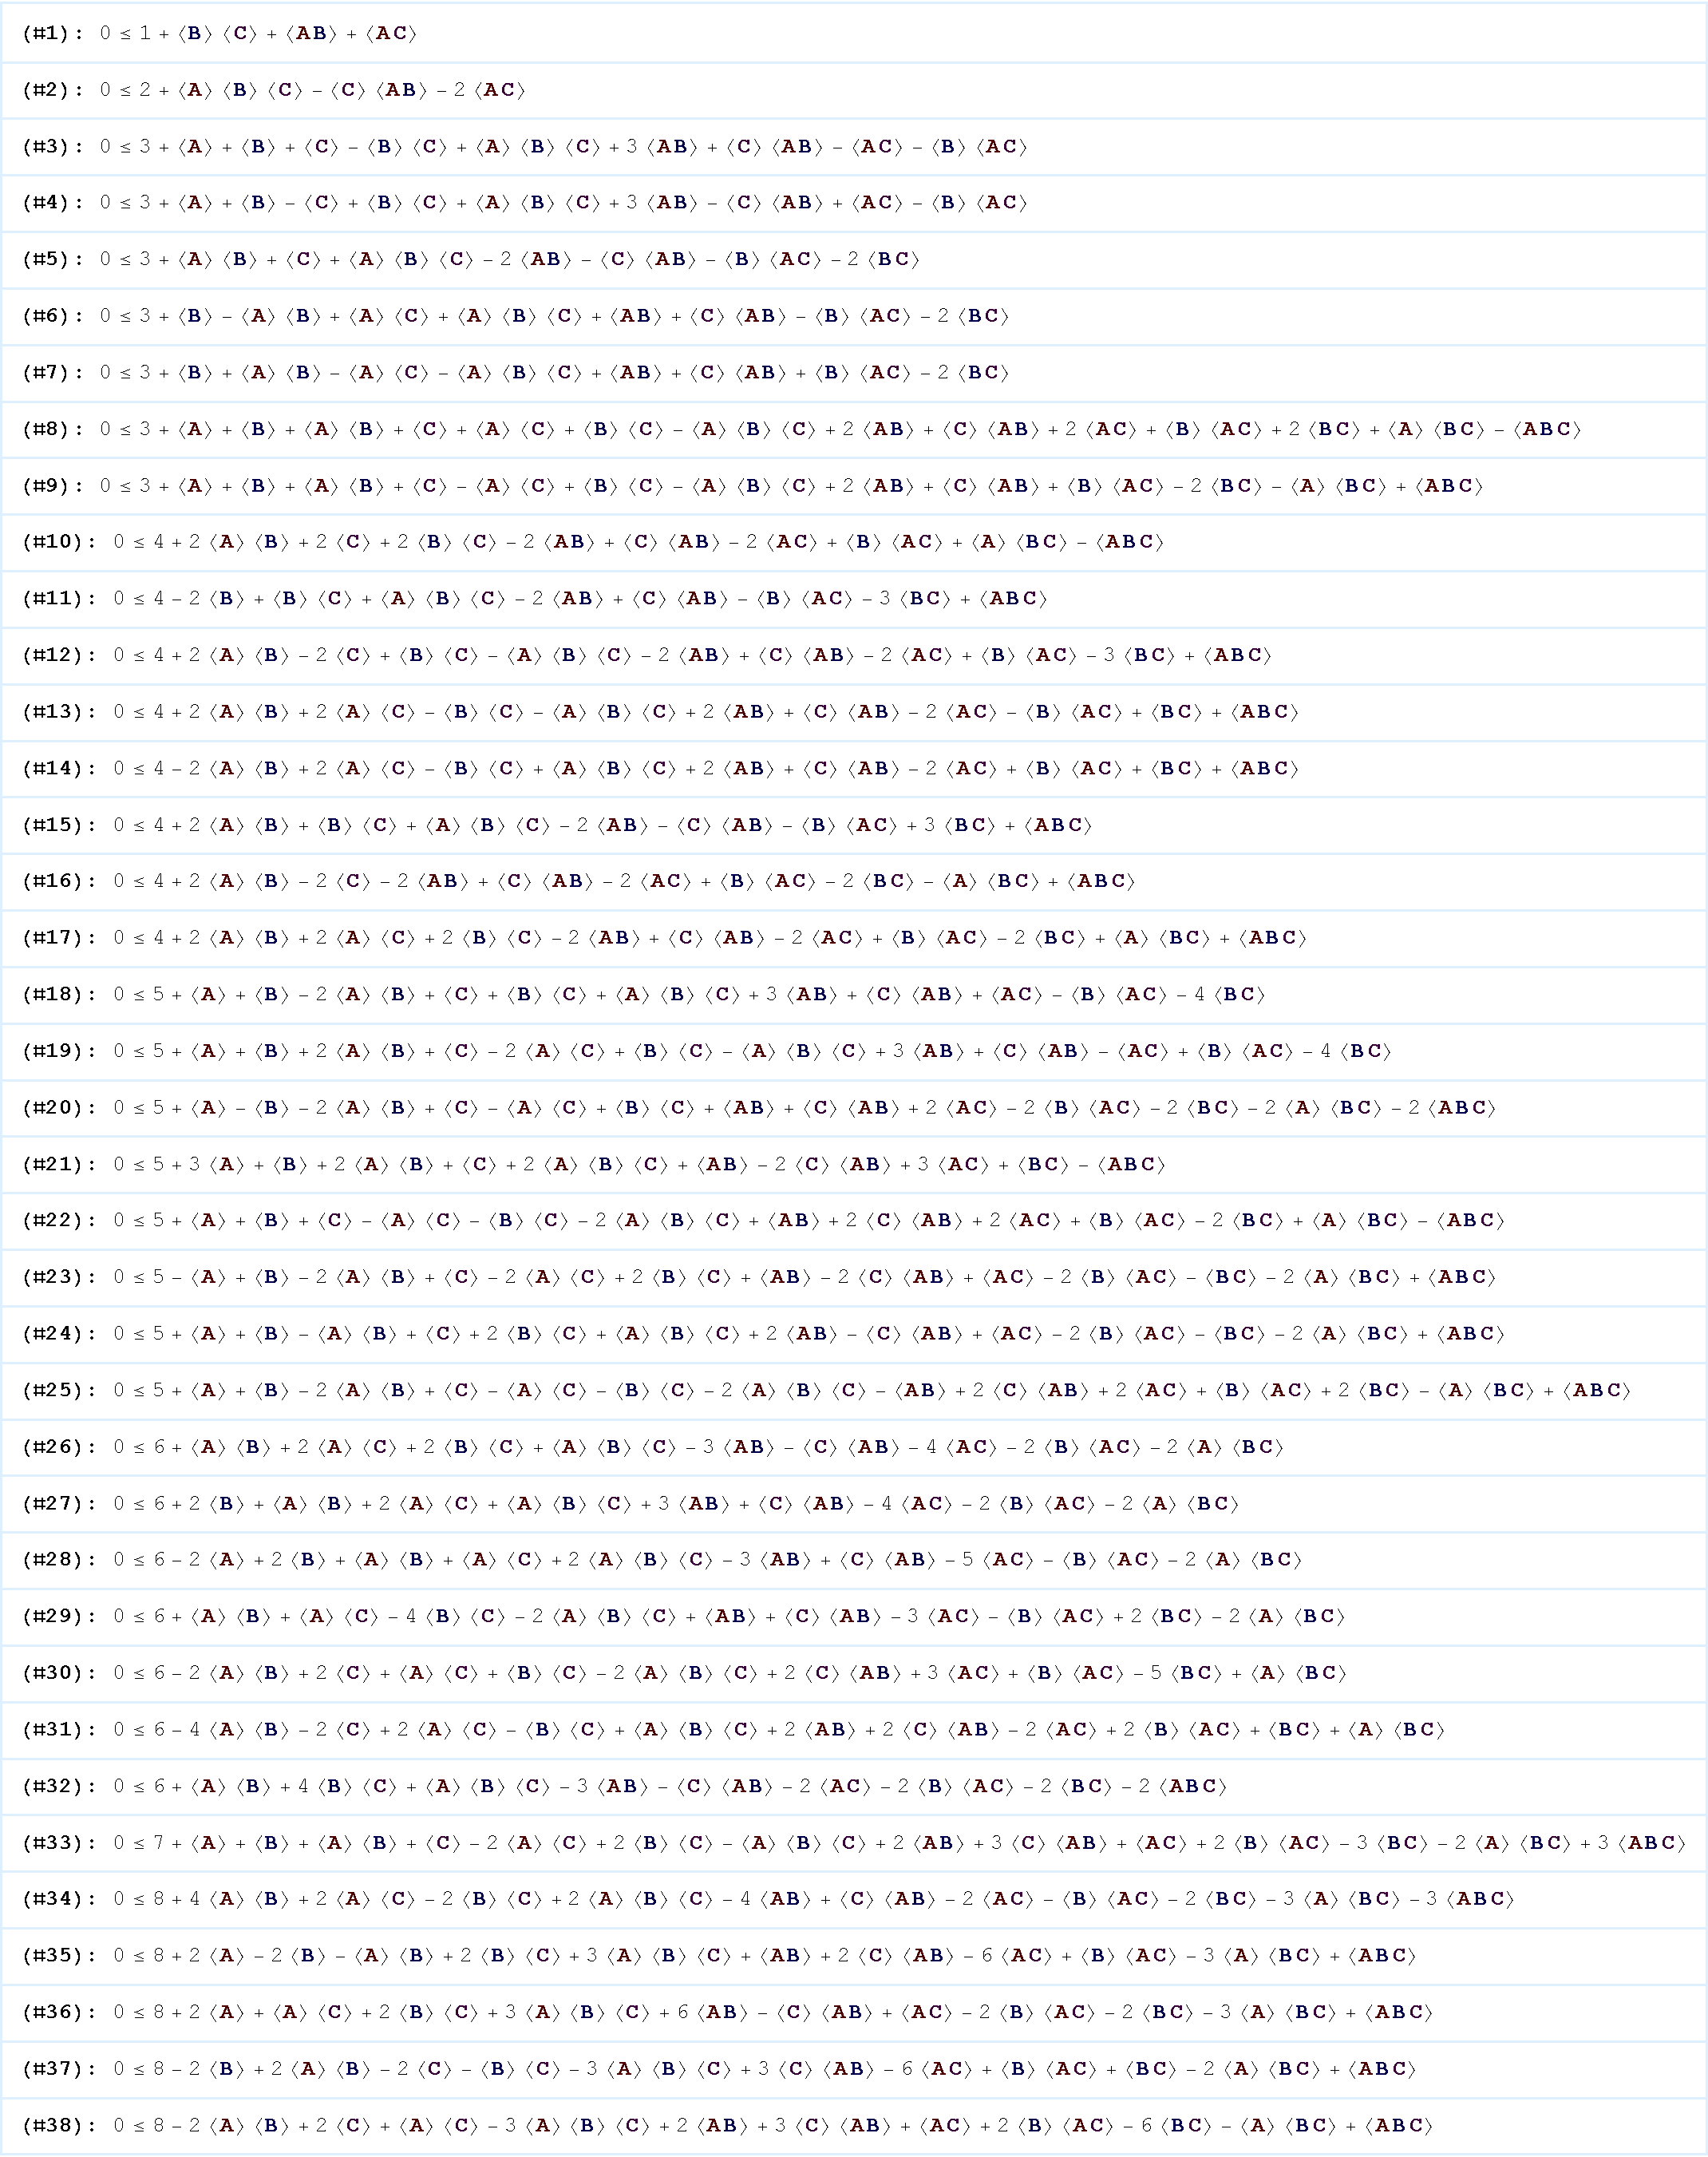
\includepdf[pages=1,scale=0.90,link,linkname=nontriv,pagecommand={\refstepcounter{includepdfpage}\label{nontriv.\theincludepdfpage}}]{nontrivlist.pdf}
%
%\begin{figure}[H]
% 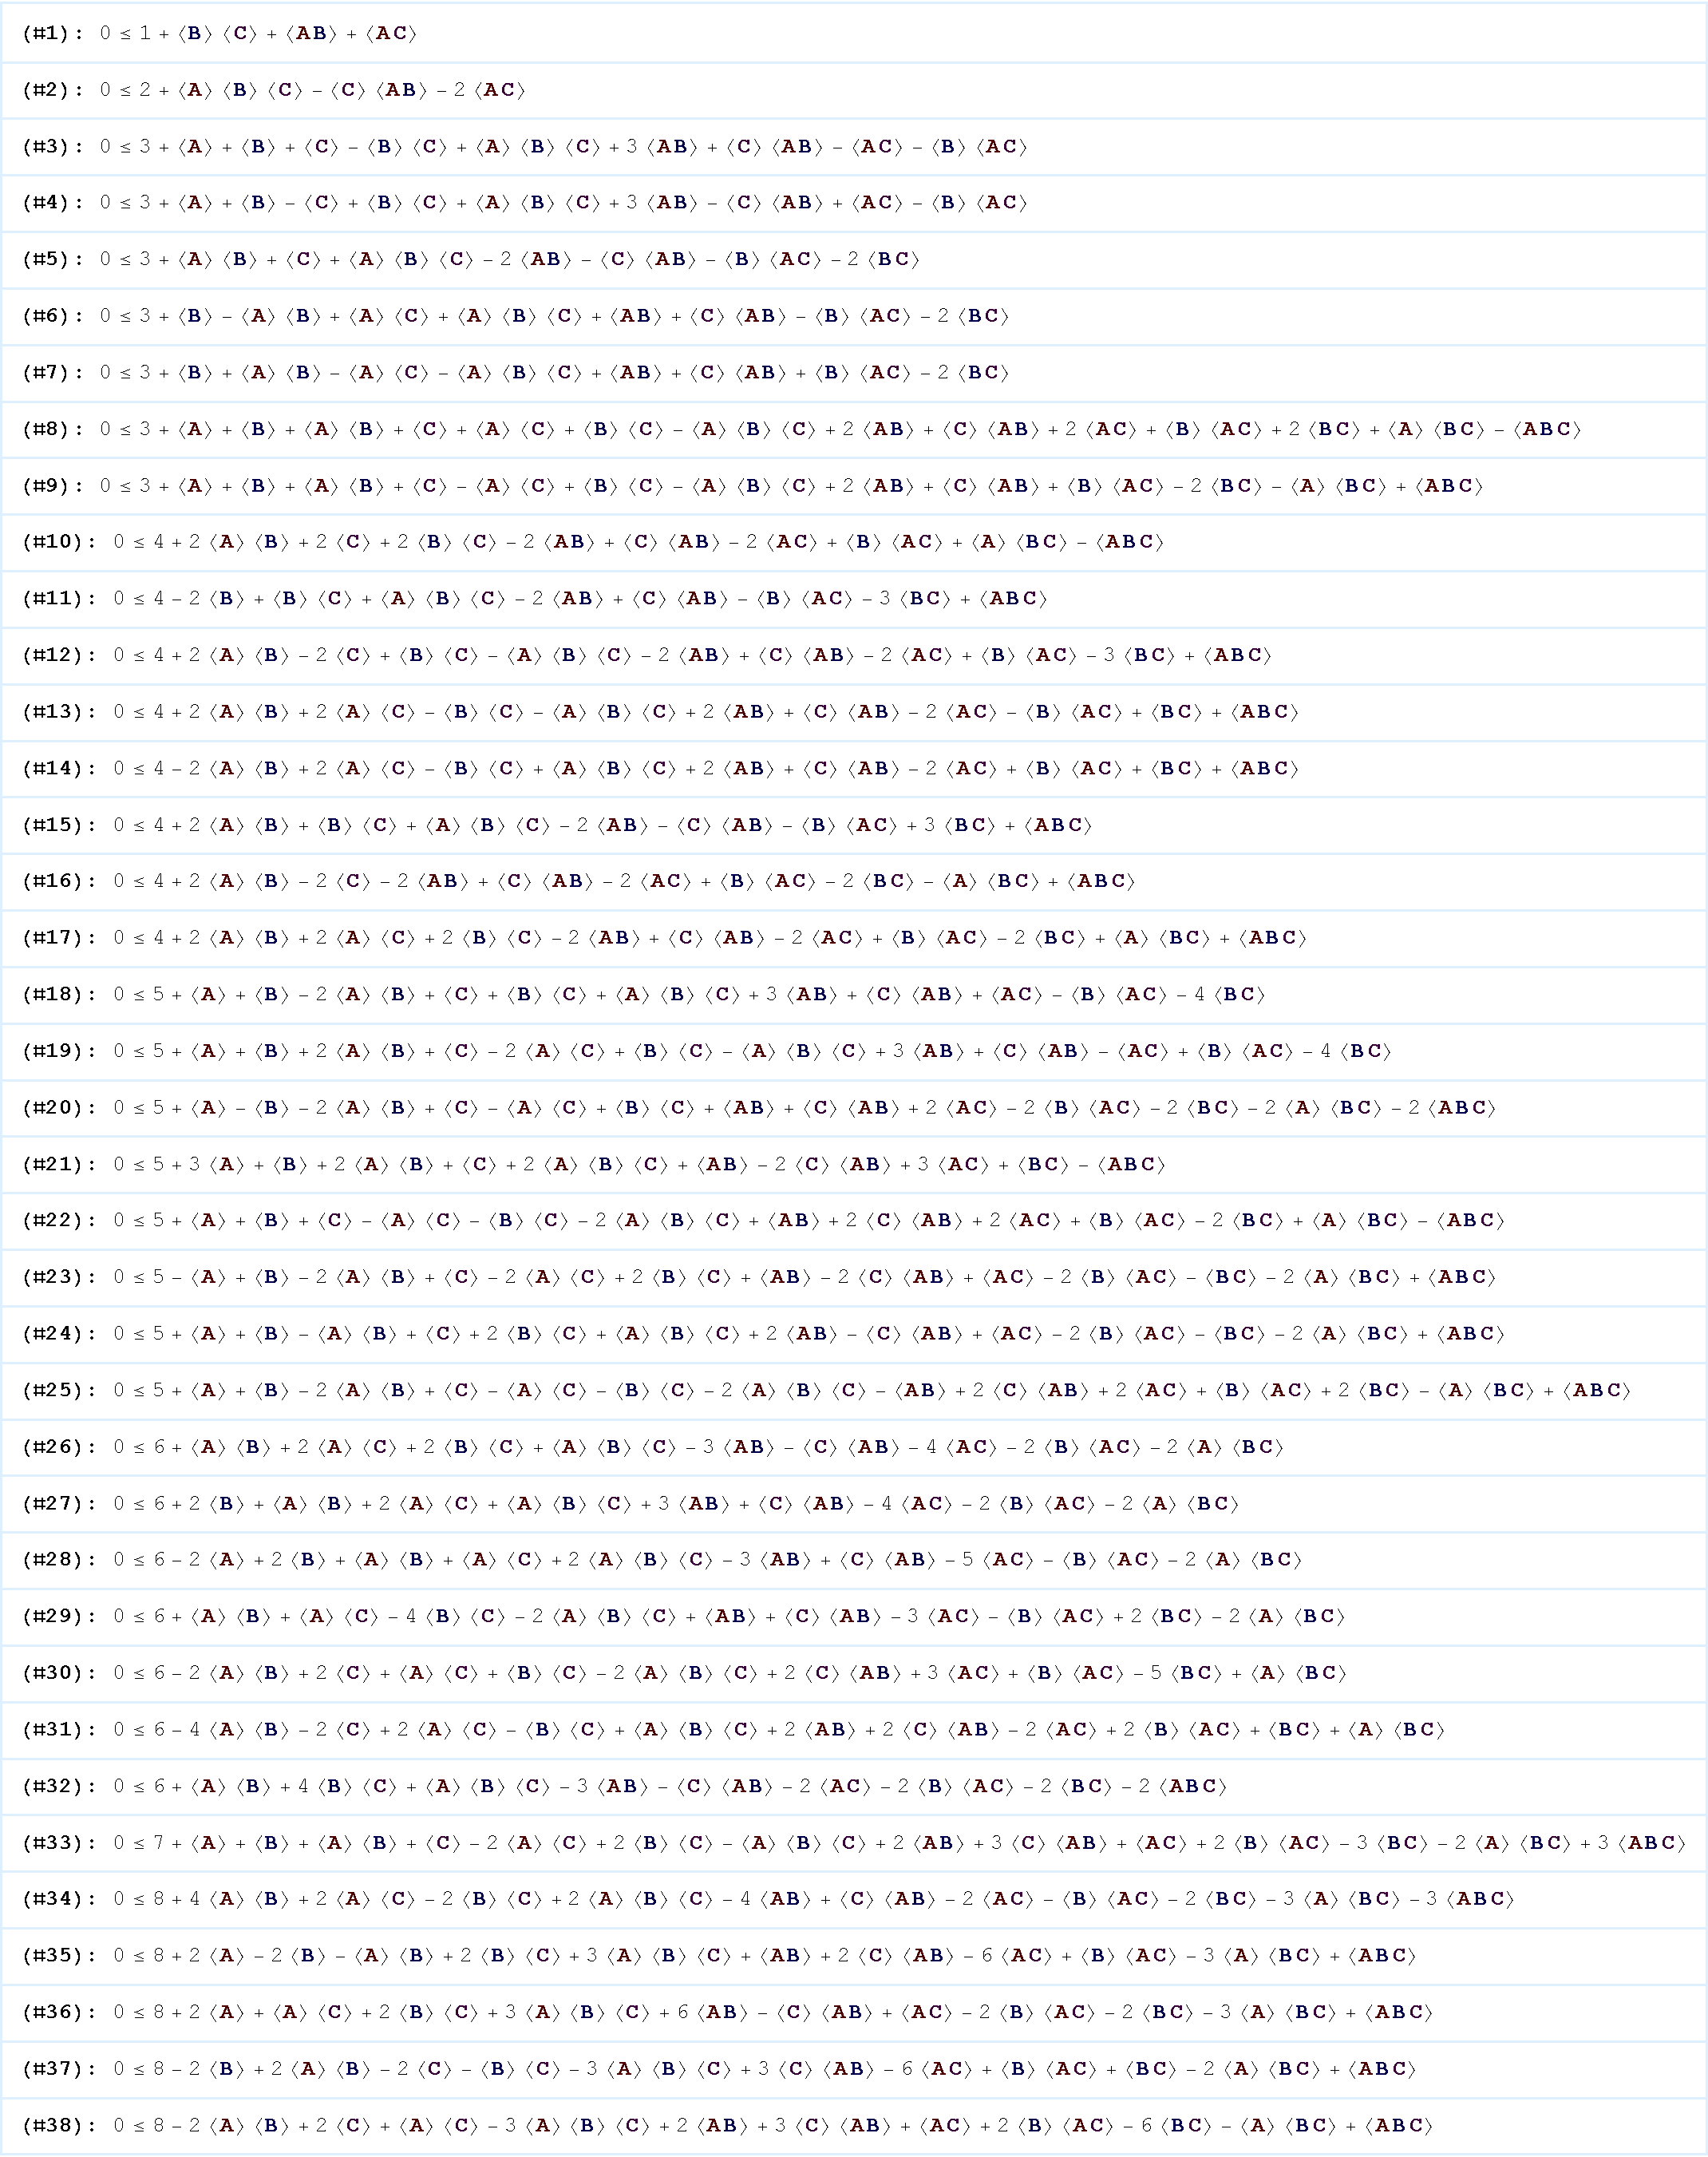
\includegraphics[width=\textwidth]{nontrivlist.pdf}\label{nontriv.humanreadable}
A star next to the index of an inequality indicates that the inequality can also be derived by considering the possibilisitc marginal problem per \cref{sec:TSEM} in lieu of solving the standard (probabilistic) marginal problem described above.
%\end{figure}
%
%


%This is the approach that we will consider in the next section.
%Note that if one merely has linear inequalities that contain the marginal polytope rather than describing its facets, one can still follow the above prescription for deriving causal compatibility inequalities.  This is the approach that we will consider in the next section.



% When solving the marginal problem is too difficult, one may consider solving a relaxation of it, instead. One extremely computationally amenable relaxation of the marginal problem is to enumerate probabilistic Hardy-type paradoxes. This is discussed later on in  \cref{sec:TSEM}.

%\topic{\tred{Constraining Possible Distributions over Pre-Injectable Sets via Hardy Paradoxes}}

%Although solving the marginal problem can be highly optimized, it can still prove computationally difficult. It is therefore sometimes useful to consider relaxations of the marginal problem. The \emph{full} marginal problem is to find inequalities on the marginal distributions such that the inequalities are satisfied \emph{if and only if} the given marginal distributions can be extended. It is much easier to generate necessary-but-insufficient inequalities, i.e. satisfied by all compatible marginal distributions but such that no-violation does not certify marginal compatibility. We have identified a technique for rapidly generating such quantifier-free inequalities by restricting the search to inequalities of a very particular form. We found this alternative technique — trading generality for speed — to be extraordinarily practical. The type of inequalities that we consider are given by a certain class of tautologies in classical propositional logic, see \cref{sec:TSEM} for further details.


%\section{Deriving Hardy-type constraints for the marginal problem}\label{sec:TSEM}
%\section{Deriving inequalities for the marginal problem from possibilistic constraints}\label{sec:TSEM}
%\subsection{The possibilistic marginal problem and its implications for the probabilistic marginal problem}\label{sec:TSEM}
%\subsection{Causal compatibility inequalities via the possibilistic counterpart to the marginal problem}\label{sec:TSEM}
\subsection{Causal compatibility inequalities via Hardy-type inferences from logical tautologies}\label{sec:TSEM}


%\color{red}
Enumerating all the facets of the marginal polytope is computationally feasible only for relatively small examples. But our method still applies when only some inequalities that bound the marginal polytope are known, and we now present a general approach for deriving such inequalities very quickly.

In the literature on Bell inequalities, it has been noticed that incompatibility with the Bell DAG can sometimes be witnessed by merely looking at which joint outcomes have zero probability and which ones have nonzero probability. In other words, instead of considering the \emph{probability} of an outcome, the inconsistency of some marginal distributions can be evident from considering only the \emph{possibility} or \emph{impossibility} of each outcome. This insight is originally due to~\citet{L.Hardy:PRL:1665}, and versions of Bell's theorem that are based on the violation of such \tblue{possibilistic constraints} are known as \tblue{Hardy-type paradoxes}~\cite{Garuccio95,CabelloHardyInequality,Braun08,Mancinska14,LSW}; a partial classification of these can be found in~\cite{Mansfield2012}.

In this approach, the constraints follow from a consideration of {\em logical relations} that can hold among deterministic assignments to the observed variables. Such logical constraints can also be leveraged to derive probabilistic constraints instead of possibilistic ones, as shown in~\cite{Pitowsky1989,Ghirardi08}. This results in a partial solution to any given (probabilistic) marginal problem. Essentially, we solve a possibilistic marginal problem \cite{Mansfield2012}, then upgrade the possibilistic inequalities into probabilistic inequalities, resulting in a set of probabilistic inequalities whose cumulative satisfaction is a necessary but insufficient condition for satisfying the corresponding probabilistic marginal problem. We now demonstrate how to systematically derive all inequalities of this type.

%We have already provided a simple example of this sort of argument in \cref{Sec:DerivingInequalities}, in the argument used to demonstrate that the marginal distributions of Eqs.~\eqref{W4}-\eqref{W7} are incompatible with the DAG depicted in Fig.~\ref{fig:Tri222v2}.   For our present purposes, it is useful to recast the argument of \cref{Sec:DerivingInequalities} into a new but manifestly equivalent form.  First, one notes that the following proposition is a logical tautology for binary variables:
%\begin{align}\begin{split}\label{tautology1}
%&\lnot [A_2 \eql 1 \land C_1 \eql 1] \bigwedge \lnot [B_2 \eql 1 \land A_1 \eql 1] \bigwedge \lnot [C_2 \eql 1 \land B_1 \eql 1] \bigwedge \lnot [A_1 \eql 0 \land B_1 \eql 0 \land C_1 \eql 0]\\
% &\qquad\implies
%\lnot [A_2 \eql 1 \land B_2 \eql 1 \land C_2 \eql 1].
%\end{split}\end{align}
%Next, one notes that the given distribution and causal structure imply that the antecedent is true while the consequent is false for every valuation in the support of the distribution, so that the distribution and causal structure together imply a contradiction.

We have already provided a simple example of a Hardy-type argument in \cref{Sec:DerivingInequalities}, in the logic used to demonstrate that the marginal distributions of \cref{W4,W1,W5} are incompatible with the DAG depicted in \cref{fig:Tri222v2}.   For our present purposes, it is useful to recast the argument of \cref{Sec:DerivingInequalities} into a new but manifestly equivalent form.    

First, for the distribution in question, we have
\begin{align} 
\begin{split}\label{WWs}
&A_2 \eql 1 \implies C_1\eql 0\\
&B_2\eql 1 \implies A_1\eql 0\\
&C_2 \eql 1 \implies B_1 \eql 0\\
\text{Never}  &\quad A_1 \eql 0\,\text{ and }\, B_1 \eql 0\,\text{ and }\, C_1 \eql 0.
\end{split}
\end{align}
From the last constraint one infers that at least one of $A_1$, $B_1$ and $C_1$ must be 1, which from the three other constraints implies that at least one of $A_2$, $B_2$ and $C_2$ must be 0, so that it is not the case that all of $A_2$, $B_2$ and $C_2$ are 1.  Thus~\cref{WWs} implies
\begin{align} \label{consequent2}
\text{Never}  \quad &A_2 \eql 1\,\text{ and }\, B_2 \eql 1\,\text{ and }\, C_2 \eql 1.
\end{align}
However, the DAG of~\cref{fig:Tri222v2} is such that $A_2$,$B_2$, and $C_2$ have no common ancestor and consequently these variables are marginally independent in any distribution consistent with this DAG.  Combining this with the fact that the marginal distribution for each of these three variables has full support implies that $A_2$,$B_2$, and $C_2$ sometimes all take the value 1, which contradicts \cref{consequent2}.  What is nice about this form of the reasoning is that the appeal to the causal structure occurs only in the very last step.  

We are here interested in recasting the argument in such a way that the appeal to {\em both} the causal structure {\em and} the form of the marginal distributions occurs only in the very last step.  This is done as follows.  The first step of the argument is to note that the following proposition is a logical tautology for binary variables (here, $\land$, $\lor$ and $\lnot$ denote conjunction, disjunction and negation respectively):
\begin{align}\begin{split}\label{tautology1}
&\lnot [A_2 \eql 1 \land C_1 \eql 1] \bigwedge \lnot [B_2 \eql 1 \land A_1 \eql 1] \bigwedge \lnot [C_2 \eql 1 \land B_1 \eql 1] \bigwedge \lnot [A_1 \eql 0 \land B_1 \eql 0 \land C_1 \eql 0]\\
 &\qquad\implies
\lnot [A_2 \eql 1 \land B_2 \eql 1 \land C_2 \eql 1].
\end{split}\end{align}
The second and final step of the argument notes that the given distribution and the given causal structure imply that the antecedent is true while the consequent is false, so that the distribution and causal structure together imply a contradiction.

%Such Hardy-type arguments for incompatibility actually only require one to be given an assignment of {\em possible} or {\em impossible} to certain valuations of variables rather an assignment of probabilities thereto. We call such assignments {\em possibilistic}.  

In our recasting of the Hardy-type argument, the first step---identifying a logical tautology among valuations of certain subsets of the variables---
can be understood as a constraint on marginal {\em deterministic assignments}, and it is a constraint that follows from logic alone.  
%It can be understood as the logical analogue of identifying a constraint on marginals distributions that holds for {\em any} joint distribution.  
It is useful to think of this first step as the logical counterpart of a consraint on marginals. 
%the marginal problem.


%Imagine that one has specified the full set of variables, denoted $\bm{X}$, together with a family of subsets of $\bm{X}$, termed contexts and denoted $(\bm{U}_1,\ldots,\bm{U}_n)$.  A \emph{joint deterministic assignment} to $\bm{X}$ specifies a joint valuation of the variables in $\bm{X}$.  A \emph{marginal deterministic assignment} for the context $\bm{U}_i$, specifies a  joint valuation of the variables in $\bm{U_i}$. Clearly, every joint deterministic assignment defines a family of marginal deterministic assignments through restriction.   For any given family of marginal deterministic assigments, one can seek to find the conditions under which therese are the restriction of some joint deteministic assignment.  [IS THAT LAST THING RIGHT?]


%As such, \cref{tautology1} can indeed be understood as a constraint on marginal possibilistic assignments.  Thinking of it this way makes it clear that witnessing incompatibility by starting with a Hardy-type logical tautology is the possibilistic analogue of deriving causal compatibility inequalities starting with a solution of the marginal problem.  More importantly, such constraints on marginal possibilistic assignments are interesting because they can be used to derive constraints on marginal distributions, as was shown by \citet{Mansfield2012}.  

We illustrate this last claim with the example just discussed.  It can be cast as a marginal scenario where the contexts are $\{A_2 B_2 C_2\}$, $\{A_2 C_1\}$, $\{B_2 A_1\}$, $\{C_2 B_1\}$, and  $\{A_1 B_1 C_1\}$.  The logical tautology \eqref{tautology1} is then a constraint on marginal determinstic  assignments for this marginal scenario.   To see how to obtain a constraint on marginal {\em distributions}, we start by rewriting \cref{tautology1} in its contrapositive form (``and" now implicit in the brackets)
\begin{align}\begin{split}\label{tautology2}
&[\mgreen{A_2 \eql 1} , \mgreen{B_2 \eql 1} , \mgreen{C_2 \eql 1}]  \implies [\mgreen{A_2 \eql 1}, C_1 \eql 1] \lor  [\mgreen{B_2 \eql 1}, A_1 \eql 1] \lor  [\mgreen{C_2 \eql 1}, B_1 \eql 1] \lor  [A_1 \eql 0 \land B_1 \eql 0 \land C_1 \eql 0].
\end{split}\end{align}
Next, we note that if a logical tautology can be expressed as
\begin{align}\label{eq:inference}
    \SmallNamedFunction{}{E_0} \implies \SmallNamedFunction{}{E_1} \lor \ldots \lor \SmallNamedFunction{}{E_n},
\end{align}
then by applying the union bound (which asserts that the probability of at least one of a set of events occuring is no greater than the sum of the probabilities of each event occuring), 
%\color{red} understand $[A2=1 \land B2=0]$ as an event in the sense of probability theory: a subset of the sample space. A logical and then stands for intersection of events, an or for union, and the implication for the subset relation. Equivalently, by the correspondence between subsets of a set and characteristic functions on the set, you can also understand $[A2 = 1 \land B2=0]$ as a Boolean-valued random variable on the sample space, and then the logical connectives have the obvious semantics. The fact that it's enough to consider deterministic assignments to prove the implication (as in my previous paragraph) then follows from the fact that these logical operations are defined pointwise. \color{black}
 one obtains
\begin{align}\label{eq:possinference}
\p{E_0}\leq \sum\limits_{j=1}^n{\p{E_j}}.
\end{align}
Applying the union bound to \cref{tautology2} in particular yields
\begin{align}\label{eq:F3rawweak}
P_{A_2 B_2 C_2}\parens{\mgreen{1} \mgreen{1} \mgreen{1}} \leq P_{A_1 B_1 C_1}\parens{0 0 0}+P_{A_1 B_2}\parens{1 \mgreen{1 }}+P_{ B_1 C_2}\parens{ 1 \mgreen{1}}+P_{A_2 C_1}\parens{\mgreen{1 } 1},
\end{align}
which is a constraint on the marginal {\em distributions}.
 
Note that this inequality allows one to demonstrate the incompatibility of the marginal distributions of \cref{W4,W1,W5} with the inflated DAG just as easily as one can with the tautology of \cref{tautology1}.  It suffices to note that the given distribution and causal structure imply that the left-hand side has nonzero probability (which corresponds to the consequent of \cref{tautology1} being false) while every term on the right-hand side has zero probability (which corresponds to the antecedent of  \cref{tautology1} begin true).
%This is a causal compatibility inequality for the inflated DAG.  It can be used to demonstrate the incompatibility of the marginal distributions of Eqs.~\eqref{W4}-\eqref{W7} with the inflated DAG because these marginal distributions assing probability 0 to all terms on the right-hand side, while these together with the causal structure imply a nonzero probability for the term on the left-hand side.  
But, of course, the inequality can witness many other incompatibilities in addition to this one.

%The truth of the proposition $[U_i = u_i]$ implies that the marginal possibilistic assignment $S_{\bm{U}_1}$ must judge the joint valuation $u_i$ to be possible.  Consequently, any logical tautology in terms of such propositions can be understood as a constraint on the marginal possibilistic assignments. 

As another example, consider the marginal problem where the variables are $\{ A,B,C\}$, with each being binary, and the contexts are the pairs $\{AB\}$, $\{AC\}$, and $\{BC\}$.  
%where the pairwise joint distributions of three variables $A$, $B$ and $C$ are given. %, and these two variables are binary with values in $\{0,1\}$. 
The following tautology provides a constraint on marginal deterministic assignments:
%A possibilistic constraint that follows from logic alone, and therefore is true regardless of the joint distribution over $A, B, C$, is this one:
%One Hardy-type possibilistic constraint which we would want to enumerate is
\begin{align}
%    \bracks{\mgreen{A \eql a}, \mgreen{C \eql c}} \implies \bracks{\mgreen{A \eql a}, B \eql b} \bigvee \bracks{B \eql \n{b}, \mgreen{C \eql c}}
 \bracks{\mgreen{A \eql 1}, \mgreen{C \eql 1}} \implies \bracks{\mgreen{A \eql 1}, B \eql 1} \lor \bracks{B \eql 0, \mgreen{C \eql 1}}.
\end{align}
(To see that this is a tautology, simply note that $E \land F  \implies  E \land F \land (G \lor \lnot G) = (E \land F \land G) \lor (E\land F \land \lnot G) \implies (E \land G) \lor (F \land \lnot G)$.) 
Applying the union bound, one obtains the following constraint on marginal distributions\footnote{This inequality is in fact equivalent to \cref{eq:polymonogamyraw}.}
\begin{align}\label{eq:trivmarginalconstraint}
	P_{AC}(\mgreen{1 1}) \leq P_{AB}(\mgreen{1} 1) + P_{BC}(0 \mgreen{1}).
\end{align}


In this section, we seek to determine, for any marginal scenario, the set of \emph{all} inequalities that can be derived in this manner.  We do so by \tblue{enumerating} the full set of constraints on marginal deterministic assignments for the given marginal scenario.
% that arise in a given marginal problem.

We outline the general procedure using 
%a slightly more sophisticated example than the one provided above. Consider 
the marginal scenario of~\cref{fig:simplicialcomplex222}, where the full set of variables is $\{ A_1, A_2, B_1, B_2, C_1, C_2\}$ and the contexts are $\{A_1 B_1 C_1\}$, $\{A_1 B_2 C_2\}$, $\{A_2 B_1 C_2\}$, $\{A_2 B_2 C_1\}$ and $\{A_2 B_2 C_2\}$, pursuant to \cref{eq:basicsetup222}.
%\begin{align*}
%	\{A_1 B_1 C_1\},\\
%	\{A_1 B_2 C_2\},\\
%	\{A_2 B_1 C_2\},\\
%	\{A_2 B_2 C_1\},\\
%	\{A_2 B_2 C_2\}.
%\end{align*}
As before, we will express the constraints on marginal deterministic assignments as logical implications with
%Now a possibilistic constraint on this marginal problem consists of a logical implication with 
a joint valuation of one of the contexts as the \tblue{antecedent} and a disjunction over contexts of joint valuations thereon as the \tblue{consequent}. In the following, we explain how to generate \emph{all} such implications which are tight in the sense that the consequent is minimal, i.e., involves as few terms as possible in the disjunction. 
%ir right-hand sides are minimal.

First, we fix the antecedant by choosing some context and a joint valuation of its variables. In order to generate all contraints on marginal deterministic assignments, one will have to perform this procedure for \emph{every} context as the antecedent and every choice of joint valuation thereof. For the sake of concreteness, we take the example of $\bracks{\mgreen{A_2 \eql 1}, \mgreen{B_2 \eql 1}, \mgreen{C_2 \eql 1}}$ as the antecedent.  
Each logical implication we consider is required to have the property 
%The consequent will be a disjunction over contexts of joint valuations for each context, with the additional property
 that any variable that appears in both the antecendent and the consequent must be given the same value in both. 
%all outcomes of variables that also occur in the antecedent carry the same outcome. 
%For the implication to be valid, the consequent must further be such that \tred{for any \emph{joint} composite outcome which extends the antecedent's marginal composite outcome, also at least one of the marginal composite outcomes in the consequent must occur.}

To formally determine all valid consequents, we first consider two hypergraphs. Hypegraphs can be represented as zero/one matrices: Let the rows correspond to nodes and the columns to hyperedges. The positions of the 1's indicates which nodes participate in which hyperedge.  %Take the set of nodes to be the disjoint union over all the contexts of all the joint outcomes which are compatible with~\eqref{eq:lhshardy}\footnote{In the left-hand side context there will thus be only one node, and one can also omit this one node without changing the result.}. 

The nodes in the first hypegraph correspond to every possible joint valuation of the variables in a context for every possible context.
The hyperedges in the first hypegraph correspond to every possible joint valuation of all the variables. A hyperedge (joint valuation) contains a node (marginal joint valuation) iff the hyperedge is an extension of the node; for example the hyperedge $\bracks{A_1 \eql 0, \mgreen{A_2 \eql 1}, B_1 \eql 0, \mgreen{B_2 \eql 1}, C_1 \eql 1, \mgreen{C_2 \eql 1}}$ is an extension of the node $\bracks{A_1 \eql 0,  \mgreen{B_2 \eql 1}, \mgreen{C_2 \eql 1}}$. In our example following \cref{fig:simplicialcomplex222}, this initial hypergraph has $5\cdot 2^3 = 40$ nodes and $2^6 = 64$ hyperedges. Indeed, in 0/1 matrix notation, this first hypegraph is identically the marginal description matrix $\bm{M}$ introduced near \cref{eq:marginalproblemgeneric}.

The second hypergraph is a sub-hypergraph of the first one. We delete from the first graph all nodes and hyperedges which contradict the outcomes supposed by the antecedent. For example, the node $\bracks{\mgreen{A_2 \eql 1}, \mred{B_2 \eql 0}, C_1 \eql 1}$ contradicts the antecedent $\bracks{\mgreen{A_2 \eql 1}, \mgreen{B_2 \eql 1}, \mgreen{C_2 \eql 1}}$. We also delete the node corresponding to the antecedent itself. In our example, this final resulting hypergraph has $2^3 + 3\cdot 2^1 = 14$ nodes and $2^3 = 8$ hyperedges.

All valid (minimal) consequents are (minimal) \tblue{transversals} of this latter hypergraph. A transversal is a set of nodes which has the property that it intersects every hyperedge in at least one node. In order to get implications which are as tight as possible, it is sufficient to enumerate only the minimal transversals. Doing so is a well-studied problem in computer science with various natural reformulations and for which manifold algorithms have been developed~\cite{eiter_dualization_2008}.

%It is then possible right-hand sides of the implications are precisely the \tblue{transversals} of this hypergraph, i.e.~the sets of nodes which have the property that they intersect every hyperedge in at least one node. In order to get implications which are as tight as possible, it is sufficient to enumerate only the \tblue{minimal transversals}. Doing so is a well-studied problem in computer science with various natural reformulations and for which manifold algorithms have been developed~\cite{eiter_dualization_2008}. We expect that this enumeration of minimal transversals will be computationally much more tractable than the linear quantifier elimination, even if one does it for every possible left-hand side of the implication.

In our example, it is not hard to check that the consequent of
\begin{align}\begin{split}\label{eq:F3implicationform}
	\bracks{\mgreen{A_2 \eql 1}, \mgreen{B_2 \eql 1}, \mgreen{C_2 \eql 1}} \quad\Longrightarrow\quad &\bracks{A_1 \eql 0, B_1 \eql 0, C_1 \eql 0} \lor \bracks{A_1 \eql 1, \mgreen{B_2 \eql 1}, \mgreen{C_2 \eql 1}} \\
	\lor\: & \bracks{\mgreen{A_2 \eql 1}, B_1 \eql 1, \mgreen{C_2 \eql 1}} \lor \bracks{\mgreen{A_2 \eql 1}, \mgreen{B_2 \eql 1}, C_1 \eql 1}
\end{split}\end{align}
is such a minimal transversal: every assignment of values to all variables which extends the assignment on the left-hand side satisfies at least one of the terms on the right, but this ceases to hold as soon as one removes any one term on the right. 

We convert these implications into inequalities in the usual way via the union bound (i.e., replacing ``$\Rightarrow$'' by ``$\leq$'' at the level of probabilities and the disjunctions by sums). For example the constraint on marginal deterministic assignments \cref{eq:F3implicationform} translates to the constraint on marginal distributions
\begin{align}\label{eq:F3rawprobform}
%    P_{A_2 B_2 C_2}\parens{\mgreen{a_2} \mgreen{b_2} \mgreen{c_2}} \leq \p{\n{a_1} \n{b_1} \n{c_1}}+\p{a_1 \mgreen{b_2 c_2}}+\p{\mgreen{a_2} b_1 \mgreen{c_2}}+\p{\mgreen{a_2 b_2} c_1}
    P_{A_2 B_2 C_2}\parens{\mgreen{1} \mgreen{1} \mgreen{1}} \leq P_{A_1 B_1 C_1}\parens{0 0 0}+P_{A_1 B_2 C_2}\parens{1 \mgreen{1 1}}+P_{A_2 B_1 C_2}\parens{\mgreen{1} 1 \mgreen{1}}+P_{A_2 B_2 C_1}\parens{\mgreen{1 1} 1}.
\end{align}
%\[
%	P_{A_2 B_2 C_2}(111) \leq P_{A_1 B_1 C_1}(000) + P_{A_1 B_2 C_2}(111) + P_{A_2 B_1 C_2}(111) + P_{A_2 B_2 C_1}(111).
%\]
Note that \cref{eq:F3rawprobform} is a strengthening of \cref{eq:F3rawweak}.  \cref{eq:F3rawprobform} was used earlier in this article as the starting point of our third example of how to derive a causal compatibility inequality for the Triangle scenario, in Sec.~\ref{Sec:DerivingInequalities} (see \cref{eq:FritzF3raw}). Because \cref{eq:F3implicationform} is the progenitor of this inequality, it can be thought of as the progenitor of the causal compatibility inequality that one derives from it, namely, \cref{eq:FritzF3}.  


Inequalities on marginal distributions that one derives from hypergraph transversals are generally weaker than those that result from a complete solution of the marginal problem. Nevertheless, many Bell inequalities are of this form, the CHSH inequality among them \cite{Ghirardi08}.  So it seems that this method is still sufficiently powerful to generate plenty of interesting inequalities. At the same time, it should be significantly easier to perform in practice than the full-fledged linear (let alone nonlinear) quantifier elimination, even if one does it for every possible antecedent.

In conclusion, linear quantifier elimination is the preferable tool for deriving inequalities for the marginal problem whenever it is computationally tractable; but whenever it is not, then enumerating hypergraph transversals presents a good alternative. %: \cref{eq:trisimplestunmapped} here corresponds to Eq. (2-4) in~\cite{Pitowsky1989}%, and \cref{eq:bellcondeq} here corresponds to Eq. (30) in Ref. \cite{Ghirardi08}

%\color{black}




\section{Further prospects for the inflation technique}\label{sec:otherprospects}

\cref{maincorollary} states that any causal compatibility inequality on the injectable sets of an inflation DAG $G'$ can be translated into a causal compatibility inequality on the original DAG $G$. Consequently any technique for deriving causal compatibility inequalities on $G'$ can potentially be amplified by the inflation technique.  As we discovered in \cref{sec:ineqs}, even weak constraints at the level of the inflated DAG can translate into strong constraints at the level of the original DAG. In the following two subsections, we consider two additional possibilities for additional constraints that might be exploited in this way towards better inequalities.

%\topic{\tred{Constraining Possible Distributions over Pre-Injectable Sets via Conditional Independence Relations}}
\subsection{Using \textit{d}-separation relations of the inflated DAG}\label{sec:fulldsep}

In Sec.~\ref{sec:ineqs}, we considered deriving causal compatibility inequalities on the inflated DAG by taking valid inequalities for the marginal polytope on the pre-injectable sets of the inflated DAG, and then making use the ancestral independences to factorize the joint distributions on the pre-injectable sets into those on the injectable sets.
% into the distributions over each of the ancestrally-independent injectable sets contained therein.  

It is natural to wonder whether one can sometimes make use of facts about the causal structure that go beyond ancestral independences.  It is standard practice, when deriving compatibility conditions for a DAG, to make use of arbitrary $d$-separation relations among variables: if, in a given DAG, $\bm{X}$ and $\bm{Y}$ are $d$-separated\footnote{The notion of $d$-separation is treated at length in~\cite{pearl2009causality,studeny2005probabilistic,WoodSpekkens,pusey2014gdag}, so we elect not to review it here.} by $\bm{Z}$, then a distribution is compatible with that DAG only if it satisfies the conditional independence relation $\bm{X}\indep\bm{Y}|\bm{Z}$. For $\bm{Z} = \emptyset$, this specializes to ancestral independence of $\bm{X}$ and $\bm{Y}$. Thus it is natural to ask: can the inflation technique also sensibly make use of other $d$-separation relations among sets of observed variables?

%The marginal problem asks about the existence of \emph{any} joint distribution which recovers the given marginal distributions. In causal inference, however, there are plenty of other constraints on the sorts of joint distributions which are consistent with some causal hypothesis. The minimal constraint embedded in any causal hypothesis is the idea of causal structure. Thus it is natural to supplement the marginal problem with additional constraints, motivated by causal structure, constraining the hypothetical distribution over observable variables of the inflated DAG.

%The most familiar causally-motivated constraints on a joint distribution are \tblue{conditional independence relations}, say among observable variables. Conditional independence relations are inferred by $d$-separation; if $\bm{X}$ and $\bm{Y}$ are $d$-separated in the (inflation) DAG by $\bm{Z}$, then we infer the conditional independence $\bm{X}\bot\bm{Y}|\bm{Z}$. The $d$-separation criterion is explained at length in~\cite{pearl2009causality,studeny2005probabilistic,WoodSpekkens,pusey2014gdag}, so we elect not to review it here.

Every conditional independence relation $\bm{X}\indep\bm{Y}|\bm{Z}$ can be expressed as a polynomial equation in terms of probabilities: while it is most commonly written as $P_{\bm{X}\bm{Y}|\bm{Z}}(\bm{x}\bm{y}|\bm{z})=P_{\bm{X}|\bm{Z}}(\bm{x}|\bm{z})P_{\bm{Y}|\bm{Z}}(\bm{y}|\bm{z})$ for all $\bm{x}$, $\bm{y}$, and $\bm{z}$, in terms of unconditional probabilities this takes on the form
\[
\forall{\bm{x} \bm{y} \bm{z}}: \p[\bm{X}\bm{Y}\bm{Z}]{\bm{x}\bm{y}\bm{z}}\p[\bm{Z}]{\bm{z}}=\p[\bm{X}\bm{Z}]{\bm{x}\bm{z}}\p[\bm{Y}\bm{Z}]{\bm{y}\bm{z}}
\]
for all $\bm{x}$, $\bm{y}$, and $\bm{z}$. Such a nonlinear constraint can be incorporated as a further restriction on the joint distributions compatible with the inflated DAG, supplementing the basic constraints of nonnegativity of probabilities for the joint distribution of the observed variables and its ancestral independences.
% of the marginal problem discussed above.

For example in \cref{fig:Tri222}, $A_1$ and $C_2$ are $d$-separated by $\{A_2 B_2\}$. Hence one can try to incorporate the constraint that 
%might incorporate the family of nonlinear equalities 
\begin{align}\label{nonlinearequality}
\forall{a_1 a_2 b_2 c_2}: \p[A_1 A_2 B_2 C_2]{a_1 a_2 b_2 c_2}\p[A_2 B_2]{a_2 b_2}=\p[A_1 A_2 B_2]{a_1 a_2 b_2}\p[A_2 B_2 C_2]{a_2 b_2 c_2}
\end{align}
 %for all $a_1$, $a_2$, $b_2$ and $c_2$. 
 Every probability that appears in such an equation, though not defined on an injectable set, can still be expressed as a marginal of the joint distribution over all observed variables.  For instance, we can express $\p[A_2 B_2]{a_2 b_2}$ as
%  like this must occur as a marginal as well, i.e.,~it can be written as a sum of various joint probabilities, as in
\begin{align}
%\begin{array}{lll}
\forall{a_2 b_2}:\;\pdf[A_2 B_2]{a_2 b_2} = \sum\nolimits_{a_1 b_1 c_1 c_2}\pdf[A_1 A_2 B_1 B_2 C_1 C_2]{a_1 a_2 b_1 b_2 c_1 c_2}.
%\forall{a_1 a_2 b_2 c_2}:&\;\pdf[A_1 A_2 B_2 C_2]{a_1 a_2 b_2 c_2} \to& \sum\nolimits_{b_1 c_1}\pdf[A_1 A_2 B_1 B_2 C_1 C_2]{a_1 a_2 b_1 b_2 c_1 c_2},\\
%\forall{a_1 a_2 b_2}:&\;\pdf[A_1 A_2 B_2]{a_1 a_2 b_2} \to\quad& \sum\nolimits_{b_1 c_1 c_2}\pdf[A_1 A_2 B_1 B_2 C_1 C_2]{a_1 a_2 b_1 b_2 c_1 c_2}
%\end{array}
\end{align}
Upon substituting such relations into~\cref{nonlinearequality}, one obtains a system of polynomial equations and inequalities in terms of the observable joint probabilities.  We can then proceed as we did before, eliminating the unknowns $\pdf[A_1 A_2 B_1 B_2 C_1 C_2]{a_1 a_2 b_1 b_2 c_1 c_2}$ from this system. The additional difficulty now is that some the equations are nonlinear. This idea even applies to some ancestral independences between sets that are not pre-injectable: for example, $A_1 A_2 B_2 \indep C_2$ is also guaranteed by \cref{fig:Tri222}, and results in a polynomial equation closely related to \cref{nonlinearequality}.
%In particular, the number of unknown quantities to be eliminated is still the same, but now the system of equations and inequalities is nonlinear. 
%Note also that incorporating such constraints also increases the number of quantifier which must be eliminated, as additional non-injectable probabilities are now featured in the equalities corresponding to conditional independence which do not appear in the unconstrained marginal problem. 

Many modern computer algebra systems have functions capable of tackling nonlinear quantifier elimination symbolically\footnote{For example \textit{Mathematica$^{_{\textit{\tiny\texttrademark}}}$}'s \href[pdfnewwindow]{http://reference.wolfram.com/language/ref/Resolve.html}{\texttt{Resolve}} command, \textit{Redlog}'s \href[pdfnewwindow]{http://www.redlog.eu/documentation/reals/rlqe.php}{\texttt{rlposqe}}, or \textit{Maple$^{_{\textit{\tiny\texttrademark}}}$}'s \href[pdfnewwindow]{http://maplesoft.com/support/help/Maple/view.aspx?path=RegularChains/SemiAlgebraicSetTools/RepresentingQuantifierFreeFormula}{\texttt{RepresentingQuantifierFreeFormula}}, etc.}. 
%One might then hope to use such software systems to rid the hybrid inequalities of the gedankenprobabilities. 
Currently, however, it is generally not practical to perform nonlinear quantifier elimination on large polynomial systems with many quantifiers. It may help to exploit results on the concrete algebraic-geometric structure of these particular systems~\cite{garcia_bayesian_2005}. 

If one is seeking merely to assess the compatibility of a {\em given} distribution with the causal structure, then one can avoid the quantifier elimination problem and simply try and solve an existence problem: after substituting the values that the given distribution prescribes for the joint outcomes on pre-injectable sets into the polynomial system in terms of the unknown global joint probabilities, one must only determine whether that system has a solution. Most computer algebra systems can resolve such \emph{satisfiability} questions quite easily\footnote{For example \textit{Mathematica$^{_{\textit{\tiny\texttrademark}}}$}'s \href[pdfnewwindow]{http://reference.wolfram.com/language/Experimental/ref/ExistsRealQ.html}{\texttt{Reduce\`{}ExistsRealQ}} function. Specialized satisfiability software such as SMT-LIB's \href[pdfnewwindow]{http://smtlib.cs.uiowa.edu/solvers.shtml}{\texttt{check-sat}} \cite{BarFT-SMTLIB} are particularly apt for this purpose.



%But also without using quantifier elimination, the nonlinear constraints can be easily accounted for numerically. Upon substituting numerical values for all the injectable probabilities, the former quantifier elimination problem is converted to simpler existence problem: Do there exist joint probabilities that satisfy the full set of linear and nonlinear constraints numerically? Most computer algebra systems can resolve such \emph{satisfiability} questions quite easily\footnote{For example \textit{Mathematica$^{_{\textit{\tiny\texttrademark}}}$} \href[pdfnewwindow]{http://reference.wolfram.com/language/Experimental/ref/ExistsRealQ.html}{\texttt{Reduce\`{}ExistsRealQ}} function. Specialized satisfiability software such as SMT-LIB's \href[pdfnewwindow]{http://smtlib.cs.uiowa.edu/solvers.shtml}{\texttt{check-sat}} \cite{BarFT-SMTLIB} are particularly apt for this purpose.
%One can also exploit the fact than any nonlinear optimizer will return an error when a set of constraints cannot be satisfied. Nonlinear optimizers include \textit{Maple$^{_{\textit{\tiny\texttrademark}}}$}'s \href[pdfnewwindow]{http://www.maplesoft.com/support/help/Maple/view.aspx?path=Optimization/NLPSolveMatrixForm}{\texttt{NLPSolve}}, \textit{Mathematica$^{_{\textit{\tiny\texttrademark}}}$}'s \href[pdfnewwindow]{http://reference.wolfram.com/language/ref/message/NMinimize/nsol.html}{\texttt{NMinimize}}, and dozens of free and commercial optimizers for \href[pdfnewwindow]{http://ampl.com/products/solvers/all-solvers-for-ampl}{\textit{AMPL}} and/or \href[pdfnewwindow]{https://neos-server.org/neos/solvers/index.html\#nco}{\textit{GAMS}}
}.

It is also possible to use a mixed strategy of linear and nonlinear quantifier elimination, such as \citet{ChavesPolynomial} advocates. The explicit results of~\cite{ChavesPolynomial} are directly causal implications of the \emph{original} DAG, achieved by applying a mixed quantifier elimination strategy. Perhaps further causal compatibility inequalities will be derivable by applying such a mixed quantifier elimination strategy to inflation DAGs.

\subsection{Using copy-index equivalence relations on the inflated DAG}\label{Sec:copyindexequivalence}
%\topic{\tred{Constraining Possible Distributions over Pre-Injectable Sets via Coinciding Marginals}}

By the definition of inflation model (\cref{def:inflat}), if two variables in the inflated DAG $G'$ are copy-index-equivalent, $A_i \sim A_j$, then each depends on its parents in the same fashion as $A$ depends on its parents in the original DAG $G$. Hence $A_i$ and $A_j$ have the same dependence on their parents.  Formally, from $A_i \sim A$ and \cref{eq:funcdependences}, we infer that $\pfunc{A_i| \Pa[G']{A_i}}=\pfunc{A|\Pa[G]{A}}$, and similarly $\pfunc{A_j| \Pa[G']{A_j}}=\pfunc{A|\Pa[G]{A}}$.  These two equations imply that 
\begin{align}\label{copyindexequivalence}
\pfunc{A_i| \Pa[G']{A_i}}=\pfunc{A_j|\Pa[G']{A_j}}.
 \end{align}
By the definition of inflation, the ancestral subgraphs of $A_i$ and $A_j$ are identical, and equations like \cref{copyindexequivalence} also hold for all their ancestors. We conclude that also the marginal distributions of $A_i$ and $A_j$ must be equal, $\pfunc{A_i}=\pfunc{A_j}$.
%for any pair of single-variable contexts corresponding to variables that differ only in their copy index, such as $A_i$ and $A_j$, the marginal distributions are equal, $ \pfunc{A_i}=\pfunc{A_j}$.
More generally, it may be possible to find pairs of contexts in $G'$ of any size such that constraints of the form of~\cref{copyindexequivalence} imply that the marginal distributions on these two contexts must be equal. 
%This condition implies that for certain pairs of marginal contexts in the inflated model, the marginal distributions on each are equal.   

%For example, 
For example, consider the pair of contexts $\brackets{A_1 A_2 B_1}$ and $\brackets{A_1 A_2 B_2}$ for the marginal scenario defined by the inflated DAG of~\cref{fig:Tri222}. Neither of these two contexts is an injectable set.  Nonetheless, because of~\cref{copyindexequivalence}, we can conclude that their marginal distributions coincide in any inflation model,
\begin{align}\label{CIEconsequence}
\forall{a a' b}:\;\p[A_1 A_2 B_1]{a a' b} = \p[A_1 A_2 B_2]{a a' b}.
\end{align}
We can also conclude that in the inflation model these marginal distributions satisfy  $P_{A_1 A_2 B_1}=P_{A_2 A_1 B_2}$---where now the order of $A_1$ and $A_2$ is opposite on the two sides of the equation---or equivalently, 
\begin{align}\label{CIEconsequence2}
\forall{a a' b}:\;\p[A_1 A_2 B_1]{a a' b} = \p[A_1 A_2 B_2]{a' a b}.
\end{align}
These constraints entail that $P_{A_1 A_2 B_2}$ must be symmetric under exchange of $A_1$ and $A_2$, which in itself is another equation of the type above.

%Indeed, even if we focus on the single context $\brackets{A_1 A_2}$, the constraint of~\cref{copyindexequivalence} implies a constraint on the marginal distribution $P_{A_1 A_2}$, namely, that it is symmetric under exchange of $A_1$ and $A_2$, 
%\begin{align}\label{CIEconsequence3}
%\forall{a a'}:\;\p[A_1 A_2]{a a'} = \p[A_1 A_2 ]{a' a}.
%\end{align}

%we can no longer describe the resulting constraints as ``coincidence'' of marginal distributions for a pair of contexts.  The resulting constraint might simply by a restriction on the marginal distribution for a single context.]  If $\varphi$ is not the identity map, then the equation $P_{\bm{U}} = P_{\bm{V}}$ is nontrivial even when $\bm{U}=\bm{V}$: in this case, it is effectively requiring $P_{\bm{U}}$ to be invariant under permuting the variables according to the automorphism $\varphi$.

Parameters such as $\p[A_1 A_2 B_1]{a_1 a_2 b}$, $\p[A_1 A_2 B_2]{a_1 a_2 b}$ and $\p[A_1 A_2]{a_1 a_2}$ can each be expressed as sums of the $\pdf[A_1 A_2 B_1 B_2 C_1 C_2]{a_1 a_2 b_1 b_2 c_1 c_2}$, so that relations such as \cref{CIEconsequence,CIEconsequence2} each constitute an additional equation that can be added to the system of equalities and inequalities that constitute the starting point of the satisfiability problem (if one is seeking to test the compatibility of a given distribution with the inflated DAG) or the quantifier elimination problem (if one is seeking to derive causal compatibility inequalities for the inflated DAG).  If any such additional constraints yield stronger constraints at the level of the inflated DAG, then they may translate into stronger constraints at the level of the original DAG.

%  incorporated into either linear or nonlinear quantifier eliminations in order to derive stronger causal compatibility inequalities. 
The general problem of finding pairs of marginal contexts in the inflated DAG for which relations of copy-index-equivalence imply equality of the marginal distributions, and the conditions under which such equalities may yield tighter inequalities, are discussed in \cref{sec:coincidingdetails}.


%Even if the original hypothesis does not constrain possible causal models beyond $d$-separation, The inflation hypothesis is (in all nontrivial cases) more than just that: every inflated model also satisfies $\pdf{A_i| \Pa{A_i}}=\pdf{A_j|\Pa{A_j}}$, per \cref{eq:funcdependences}.
% Consequently, the distributions over different injectable sets must occasionally coincide, i.e. $\pdf{\bm{X}}=\pdf{\bm{Y}}$ whenever both $\bm{X}$ and $\bm{Y}$ are injectable, and $\subsim{\bm{X}}=\subsim{\bm{Y}}$.

%This implies cases that distributions over certain sets of nodes must coincide in any inflated model. For example, $P_{\bm{X}} = P_{\bm{Y}}$ certainly holds whenever $\bm{X}$ and $\bm{Y}$ are injectable and $\subsim{\bm{X}} = \subsim{\bm{Y}}$, but adding this constraint to the quantifier elimination problem does not help as both sides of this equations are already determined by the original distribution. However, this type of equation also follows in some cases when $\bm{X}$ and $\bm{Y}$ are not injectable. 
%For example, $P_{A_1 A_2 B_1}=P_{A_1 A_2 B_2}$ follows from \cref{fig:Tri222} and the inflation hypothesis, even though $\brackets{A_1 A_2 B_1}$ and $\brackets{A_1 A_2 B_2}$ are not injectable sets.

%Hence equations such as 
%\begin{align}
%\forall{a_1 a_2 b}:\;\p[A_1 A_2 B_1]{a_1 a_2 b} = \p[A_1 A_2 B_2]{a_1 a_2 b}
%\end{align}
% are true of the inflated model and consequently can be  incorporated into either linear or nonlinear quantifier eliminations in order to derive stronger causal compatibility inequalities. The details of how to recognize coinciding distributions beyond the obvious coincidences implied by injectable or pre-injectable sets and under what conditions they may yield tighter inequalities are discussed in \cref{sec:coincidingdetails}.



%One may also substitute numeric values for all the pre-injectable probabilities appearing in the marginal problem. Upon doing so, the quantifier elimination problem is converted to a quantifier existence problem: Do there exist gedankenprobabilities that satisfy the resulting system of inequalities? Such \emph{satisfiability} questions can be resolved quite rapidly, especially when the quantifiers are linear \cite{Korovin2012ImplementingCRA,Bobot2012SimplexSAT}. Note that real-world data with uncertainties can also be incorporated into these satisfiability questions. Instead of asserting that a particular probability is equal to a given \emph{value}, one can incorporate new inequalities which constrain the experimentally-known probabilities to lie in given \emph{intervals}. Assigning probabilities to intervals as opposed to numeric values results in further free parameters in the system, but the problem nevertheless remains one of \emph{universal} existential closure, and can be resolved with extreme efficiency.


%One useful alternative to linear quantifier elimination is to identify representative probability distributions which are incompatible with the (unprojected) constraints; \citet{ChavesNoSignalling} use this technique, for example. %That technique essentially translates the elimination problem to a satisfiability problem, and moreover an ultra-efficient \emph{linear} quantifier existence problem at that! In the context of polytope projection, these representative probability distributions correspond to extreme rays of the so-called ``projection cone" \cite{jones2004equality,Jones2008,BalasProjectionCone}.

%A final alternative to linear quantifier elimination is to restrict one's consideration to quantifier-free inequalities with a particular form. We found this alternative technique — trading generality for speed — to be extraordinarily practical. The subtype of causal criteria which can be most rapidly recognized are those which follow from certain tautologies in classical propositional logic, see \cref{sec:TSEM} for further details.




%\purp{It is interesting to compare the technique for deriving polynomial inequalities here to that in in Ref. \cite{ChavesPolynomial}. On the one hand, our initial set of linear inequalities is much stronger, as we work with the inflated DAG whereas \citet{ChavesPolynomial} considers only the original DAG. This allows us to analyze scenarios which Ref. \cite{ChavesPolynomial} cannot, namely those without any observable conditional independence relations, such as the Triangle scenario. On the other hand, Ref. \cite{ChavesPolynomial} purportedly incorporates any kind of observable conditional independence relation, whereas we account only for \emph{unconditional} independence relations, per \cref{step:fac}. A careful examination of Ref. \cite{ChavesPolynomial}, however, reveals that only unconditional independence relations are utilized in all the examples there. To that extent, therefore, all the explicit results in Ref. \cite{ChavesPolynomial} are implied by the inflation technique.}

%We note that our polynomial inequalities are related to those introduced recently by \citet{ChavesPolynomial}, in that our inequalities subsume the explicit results of Ref. \cite{ChavesPolynomial}. \purp{NEEDS CONFIRMATION!} \citet{ChavesPolynomial} exploits conditional independence at the observable level only, whereas our technique is applicable to scenarios even without any observable CI relations, such as the Triangle scenario.



\color{black}


\subsection{Causal inference in quantum theory and in generalized probabilistic theories\label{sec:classicallity}}
%\section{Quantum Causal Inference and the No-Broadcasting Theorem}\label{sec:classicallity}


%In the causal inference problems with latent nodes that we have considered so far, the latent nodes correspond to unobserved random variables. In \emph{quantum} physics, however, the latent nodes may instead represent \emph{quantum systems}. 

Recent work has sought to explore quantum generalizations of the notion of a causal model, termed {\em quantum causal models} \cite{pusey2014gdag,BeyondBellII,Chaves2015infoquantum}.  The causal structures are still represented by DAGs, but (i) the classical random variable on every latent node is generalized to a quantum system on a Hilbert space, and (ii) the conditional probability distribution in which a node depends causally on its parents is generalized to a completely positive trace-preserving map.
  %each latent node represents a quantum system associated to a complex Hilbert space and the way in which it depends causally on its parents is represented by a completely-positive trace-preserving linear map.  
A quantum causal model is still ultimately in the service of explaining joint distributions over classical variables.  These variables represent the settings of preparation procedures and the outcomes of measurements that are used in an experiment on quantum systems, and the statistical distribution over such variables is the only experimental data with which one can confront a given quantum causal model.  The basic problem of causal inference for quantum causal models, therefore, concerns the compatibility of a joint distribution over observed classical variables with a given DAG when the model supplementing the DAG is quantum. If this happens, we say that the distribution is {\em quantumly compatible} with the DAG.  
 
%[provide definition of a quantum causal model?]

One motivation for studying quantum causal models is that they offer a new perspective on an old  problem in the foundations of quantum theory: that of establishing precisely which of the principles of classical physics must be abandoned in quantum physics. \citet{WoodSpekkens} showed that Bell's theorem~\cite{bell1966lhvm} can be leveraged to prove that there exist distributions over observed variables (predicted by quantum theory and observed experimentally \cite{Brunner2013Bell}) that cannot be accounted for in the Bell scenario under any classical causal model without doing violence to fundamental principles of causal inference such as Reichenbach's principle and the principle that conditional independences should not be fine-tuned (the principle of faithfulness). 
Quantum causal models, on the other hand, {\em can} account for these distributions in the Bell scenario.  In other words, although these distributions are not {\em classically} compatible with the Bell scenario, they are {\em quantumly} compatible with it.  Furthermore, such quantum causal explanations suggest \cite{leifer2013conditionalstates,Spekkens2015paradigm,henson2011ontic} that quantum theory is perhaps best understood as revising our notions of the nature of unobserved entities, how one represents causal dependencies thereon and incomplete knowledge thereof, while 
%the innovation of quantum theory may be best understood as an innovation to how one represents incomplete knowledge of unobserved entities (the latent nodes), while 
nonetheless {\em preserving} the spirit of Reichenbach's principle and the principle of no fine-tuning. 
% is represented while offer the possibility of securing causal explanations of such distributions while maintaining the spirit of these principles.

Another motivation for studying quantum causal models is a practical one.  Violations of Bell inequalities have  been shown to constitute resources for information processing \cite{NoSigPolytope,scarani2012device,BancalDIApproach}.   To witness such an advantage, it may seem necessary that a given information processing task can be recast in such a way that the causal structure of the protocol mirrors that of the Bell scenario.  Many tasks, however, may not be amenable to being cast in this form.  And yet the Bell scenario is not the only DAG for which there exist distributions that are quantumly but not classically compatible.
 %one can identify distributions that are quantum compatible but  where there is a separation between the distributions consistent with a quantum causal model and those consistent with a classical causal model. 
It has been shown that such a separation also exists 
%not just for the Bell scenario, but for other causal structures as well, such as
in the bilocality scenario \cite{BilocalCorrelations} and the Triangle scenario~\cite{fritz2012bell}, and it is likely that many more DAGs with this property will be found.  The hope, therefore, is that for any DAG where one can identify a quantum-classical separation, some of the separating distributions may constitute a resource for information processing. 
%achieving a quantum-classical separation in novel DAGs might, like distributions that violate the Bell inequalities, be resources for information processing.

%In a causal model, each latent node of the causal structure represents a random variable and the way in which a node depends causally on its parents is represented by a conditional probability distribution.  In the field of quantum foundations, however, there has recently been interest in defining a quantum generalization of the notion of a causal model---a quantum causal model---wherein the latent nodes instead represent \emph{quantum systems} and the way in which a node depends causally on its parents is represented by a completely-positive trace-preserving map. 

%Whenever this is allowed, we say that the DAG represents a \tblue{quantum causal structure}. Some quantum causal structures are famously capable of generating distributions over the observed variables that would not be possible classically\footnote{The incompatibility of quantum correlations with practical causal structure which generates them is known as Bell's theorem \cite{bell1966lhvm}. The particular distributions which violate Bell inequalities are known as nonlocal correlations~\cite{Brunner2013Bell}. Although the term suggests the existence of nonlocal interactions, in the sense that the actual causal structure may be different from the hypothesized one, this interpretation is at odds with the fact that no nonlocal interactions have been observed in nature, implying that their presence would require fine-tuning~\cite{WoodSpekkens}. A less problematic alternative conclusion from Bell's theorem is the impossibility to model quantum physics in terms of the usual notions of ``classical'' probability theory.}.

So for both foundational and practical reasons, there is a strong motivation to find examples of DAGs that exhibit a quantum-classical separation.
%and distributions over its observed variables such that the distribution is compatible with a quantum causal model on the DAG but incompatible with a classical causal model. 
%, or to show that there is no separation. 
However, this is by no means an easy task.
The set of distributions that are quantumly compatible with a given DAG is actually very similar to the set of distributions that are classically compatible with that DAG~\cite{pusey2014gdag,fritz2012bell}. For example, both the classical and quantum sets respect all the conditional independence relations among observed nodes that are implied by the $d$-separation relations of the DAG~\cite{pusey2014gdag}, and entropic inequalities are only of very limited use~\cite{chaves2012entropic,fritz2012bell}. We hope that our methods will provide better tools for this purpose.
% It is an interesting problem to find distributions that are realizable quantumly but not classically on a given DAG, or to show that there are no separation. 
%However, this is by no means an easy task. For example, 
%a Shannon-type entropic inequality on observed variables that is derived from the Markov conditions on all nodes \cite{chaves2012entropic,fritz2012bell}. Fine-graining the scenario by conditioning on root variables (``settings'') leads to a different kind of entropic inequality, and these have proven somewhat quantum-sensitive \cite{braunstein1988entropic,SchumacherInequality,chaves2014novel}. Such inequalities are still limited, however, in that they only apply to DAGs that include root nodes that are observed\footnote{Rafael Chaves and E.W.~are exploring the potential of entropic analysis based on considering distributions conditioned on \emph{non}-root observed nodes. Jacques Pienaar has alluded to similar considerations as a possible avenue for further research as well \cite{pianaar2016interesting}.}, and they still fail to witness cases of classical incompatibility of certain distributions with a given DAG where the incompatibility is witnessed by other techniques~\cite{chaves2014novel,fritz2012bell}.

%Some constraints on compatibility can be proven to apply not only to quantum generalizations of causal models, but also to {\em postquantum} generalizations as well~\cite{pusey2014gdag}. 

In addition to quantum generalizations of causal models, one can define generalizations for other operational theories that are neither classical nor quantum, as was done in~\cite{pusey2014gdag} and in a slightly less general setup in~\cite{BeyondBellII}.
%also define {\em postquantum} generalizations thereof, as was done in Henson, Lal and Pusey~\cite{pusey2014gdag}.
%The latter notion is
Such generalizations are formalized using the framework of {\em generalized probabilistic theories} (GPTs) \cite{Barnum2012GPT,Janotta2014GPT}, a framework that is sufficiently general to describe any operational theory that makes statistical predictions about the outcomes of experiments and passes some basic sanity checks.  Some constraints on compatibility can be proven to apply not only to classical and quantum causal models, but to any theory expressible in this framework.  %{\em postquantum} generalizations as well.  
These are the {\em theory-independent} limits on correlations of Ref.~\cite{pusey2014gdag}.  They are of interest because they clarify what any conceivable theory of physics can achieve in a given causal scenario. For example, the classically-valid conditional independence relations implied between observable variables in a DAG are all also valid in the GPT framework\cite{pusey2014gdag}. Consequently, a DAG cannot exhibit \emph{any}  GPT-quantum or even GPT-classical separation whenever the set of distributions (classically) compatible with the given DAG is \emph{precisely} picked out by the the conditional independence relations among observed nodes that implied by $d$-separation; see \cref{sec:interestingproof}.

The Bell scenario is known to manifest a GPT-quantum separation, through the work of Tsirelson \cite{Tsirelson1980} and \citet{PROriginal}.  The identification of such stronger-than-quantum correlations in the Bell scenario has been a focus of much foundational research in recent years.  Traditionally the foundational question has always been: why does quantum theory predict correlations that are {\em stronger} than one would expect classically?  But now there is a new question being asked: why does quantum theory predict correlations that are {\em weaker} than those predicted by other GPTs?  There has been some interesting progress in identifying physical principles that can pick out the precise degree of correlations that are exhibited by quantum theory \cite{PopescuReviewNatureComm,ScaraniML,Rohrlich2014,InfoCausArXiv,LOExploring,EPNBody,barnum2014interference,AlmostQuantum}.  Further opportunities for identifying such principles would be useful.  This motivates a classification of DAGs into those which have a quantum-classical separation, those which have a GPT-quantum separation and those which have both. 

Is is similarly desirable to classify (classical) causal compatibility \emph{inequalities} into those criteria which are GPT-valid, those which are GPT-violable-but-quantum-valid, and those which are quantum-violable. 

%By classifying causal compatibility inequalities by whether-or-not they hold in the GPT or quantum frameworks, one can seek to identify DAGs that exhibit a GPT-classical separation or a GPT-quantum separation, that is, to identify DAGs for which there exist distributions that are GPT compatible but not classically compatible (respectively not quantumly compatible) with the DAG. 

% one can identify DAGs that exhibit a GPT-classical separation, that is, for which there exist distributions that are GPT compatible but not classically compatible with the DAG.  
 
%Consider GPT-classical separation first. A sufficient condition for \emph{no} GPT-classical separation was provided in~\cite{pusey2014gdag}. Of the classes of DAGs with six or fewer nodes identified therein as being potentially \emph{interesting} (by not satisfying a sufficient condition for being uninteresting), all but three classes were demonstrated to indeed be interesting.  \citet{pianaar2016interesting} recently demonstrated that the three remaining classes are interesting as well.  In \cref{sec:interestingproof} we show how the inflation technique provides an alternative means of demonstrating the interestingness of one of these three classes. 
%can also be used to demonstrate a GPT-classical separation for one of these three cases. 

%Finally, one can seek to identify DAGs that exhibit a separation between GPT causal models and quantum causal models.  

%Finding GPT-quantum separations is likely a difficult quantitative task, as it is not clear how to generally isolate causal compatibility inequalities which are quantumly-valid but also GPT-violable.
%A sufficient and conjectured-necessary condition for a DAG
% is likely to yield further insights into the principles underlying the quantum formalism.  

%A slightly easier problem than characterizing 

%{\color{purple}  Mention that the distinction between whether the nodes of the DAG represent variables or quantum algebras or post-quantum things is something that is part of the causal parameters, not the causal structure.  We must therefore revise our description of a causal model to accommodate quantum and post-quantum causal models.  Specifically, we drop the claim that the nodes are variables.  Fortunately, the notion of observed versus latent and of the cardinality of an object can be made theory-independent. ---RWS}

The difference between classical, quantum and GPT causal models is the manner in which latent nodes are represented as well as the manner in which the causal influence of a latent node on other nodes is represented.  (It shares, however, the feature that the entitites that represent such causal influences mirror the causal structure---for instance, in all cases, the state of a pair of root nodes in the DAG is presumed to factorize. )
%wo subgraphs nodes that are ancestrally independent  in the graph are always represented as factorizing 
% Unlike other techniques for deriving constraints on compatibility, the inflation technique considers only the {\em observed nodes}, so it is not clear, at first glance, how it could hope to see such differences. 

%Henson, Lal and Pusey\cite{pusey2014gdag} sought to derive causal compatibility inequalities that are necessary conditions on compatibility relative to {\em any} GPT (including classical and quantum theories).  This motivated them to avoid any reference to the latent nodes...

Henson, Lal and Pusey\cite{pusey2014gdag} were able to identify constraints on compatibility that hold for {\em any} GPT by  avoiding making reference to the latent nodes of the DAG (which are treated differently in different GPTs) and only making reference to the observed variables in the DAG.   
%In [Henson, Lal, Pusey], it was shown that under the constraints that ..., one can derive causal compatibility inequalities that are necessary conditions on compatibility relative to {\em any} GPT. 

The inflation technique also only makes reference to the observed nodes in a DAG.  In some cases, the inequalities one thereby derives hold for the GPT notion of compatibility.  Indeed, the inequality for the triangle scenario that we presented in \cref{eq:polymonogamy} is the probabilistic version of the one that Henson Lal and Pusey derive in their article, and---as we already noted---in this case, their proof technique can be understood as an instance of the inflation technique. 

Nonetheless, the inflation technique also yields inequalities that hold only for the {\em classical} notion of compatibility; it is for this reason that it can be used to derive inequalities that are quantumly violated.  For instance, in \cref{example:noPR} of \cref{subsec:witnessingincompat} and \cref{sec:Bellscenarios}, we have shown how the inflation technique can be used to derive Bell inequalities, which clearly admit quantum violations. The inflation technique can be used to derive inequalities of the sort which admit quantum violations for the Triangle scenario as well \cite{TC2016trianglequantum}.

It is possible that one could generalize the inflation technique to derive inequalities that can achieve a GPT-quantum separation. This, however, requires a careful definition of a quantum causal model and is beyond the scope of this article.  Nonetheless, we will note below in which inflation in the quantum context will differ from its classical counterpart. 
%For the moment, however, we 

Our main focus here, however, will be to explain 
%We here restrict ourselves to explaining 
what distinguishes applications of the inflation technique that yield inequalities for GPT compatibility from those that yield inequalities for classical compatibility.   The distinction rests on a structural feature of the inflated DAG, which we now define.

%As noted earlier in this article, the inflation technique also refers {\em only} to the observed nodes in a DAG.  Indeed, this is one of its strengths.  \sout{However, this same fact may suggest, at first glance, that the technique will only causal compatibility inequalities of the sort derived by HLP, that is, inequalities that are necessary conditions for compatibility in {\em all} GPTs.  At first glance, therefore, it might seem that the inflation technique will be unable to distinguish classical compatibility, quantum compatibility, and GPT compatibility. }

%This is clearly not a concern given that we ruled out PR-box correlations. Also we witness the incompability of Tobias's distribution with the triangle scenario by solving the satisfiability problem.  How can that be?  How does one understand that?


\begin{definition}
A DAG $G'\in\SmallNamedFunction{Inflations}{G}$, is said to contain an \tblue{inflationary fan-out} if it contains a latent node that has two or more children that are copy-index equivalent.  
\end{definition}

The inflations of the triangle DAG that are depicted in \cref{fig:TriFullDouble} and \cref{fig:Tri222} contain one or more inflationary fan-outs, as does the inflation of the Bell DAG that is depicted in \cref{fig:BellDagCopy1}.  On the other hand, the simplest inflation of the triangle DAG that we consider in this article, that of \cref{fig:simplestinflation}, does not contain any inflationary fan-outs.
%Examples of inflated DAGs that exhibit inflationary fan-out are \cref{fig:TriFullDouble}, \cref{fig:Tri222},  and \cref{fig:BellDagCopy1}, while an example of an inflated DAG that does not is ~\cref{fig:simplestinflation}.

%Some inflations, such as the one of~\cref{fig:simplestinflation}, do not require such broadcasting. By removing $A_1$ from the broadcasting inflation of \cref{fig:simpleinflation} we obtain the non-broadcasting inflation of \cref{fig:simplestinflation}. In \cref{fig:simplestinflation} the channel from $X$ to $A$ is merely \emph{redirected} from it original configuration in \cref{fig:TriMainDAG}; there is no broadcasting of information required.

In the classical context, for every inflationary fan-out, all of the copy-index-equivalent children of the latent node are required to causally depend on the latent node in precisely the same way as their counterparts in the original DAG did.  However, the only maps that can achieve such a duplication of dependencies, known as {\em broadcasting maps}, are not physically realizable, as was famously shown for quantum theory in Ref.~\cite{NoCloningQuantum1996} and generalized to GPTs in Ref.~\cite{NoCloningGeneral2006}.  These no-broadcasting results are related to the monogamy of entanglement in quantum theory \cite{wootters2001monogomy,winter2004monogomy} (see also the discussion of the quantum conditional problem in Ref.~\cite{leifer2013conditionalstates}).  Mathematically, there {\em are} linear maps that can achieve broadcasting, as shown in \cite{Coecke2011}, but if one used these to define the inflation of a quantum causal model, then distributions over certain sets of variables in the inflated DAG (those containing the children of an inflationary fan-out) might fail to be nonnegative.  Such inflations might still be useful as a mathematical tool for ultimately deriving causal compatibility inequalities on the original DAG, but one would need to proceed differently from the way we have proceeded in this article: whereas we have here assumed that all joint valuations of the set of observed variables on the inflated DAG are nonnegative, one could not impose such a constraint for the type of quantum inflation just described.  Rather than demanding nonnegativity of the full joint distribution, one could only demand nonnegativity for distributions on sets of variables that did not include multiple children of an inflationary fan-out.  Note that the inflated DAG in such cases could not be interpreted as a causal structure.  Rather, it would be interpreted as describing multiple different {\em counterfactual} scenarios within which the causal dependencies are the same. 

%From this perspective, a broadcasting inflated DAG is an abstract logical concept, as opposed to a feasible physical construct. However, this would result in a joint distribution over all observable variables that may have some negative probabilities, and one cannot expect~\cref{eq:nonnegativity} to hold in general. But one can still try to reformulate the marginal problem so as to refer only to the existence of joint distributions on non-broadcastings sets rather than the existence of a full joint distribution from which the marginal distributions might be recovered. Here, a set $\bm{U}$ of observable nodes is non-broadcasting if $\An{\bm{U}}$ does not contain two distinct copies of a node both sharing a common latent parent.

An analysis along these lines has already been carried out successfully by \citet{Chaves2015infoquantum} in the derivation of entropic inequalities that capture quantum compatibility. Although \citet{Chaves2015infoquantum} do not invoke the inflation technique, they do seem to employ a similar type of structure to model the conditioning of an observed variable on a ``setting'' variable, a structure that we would describe as an inflated DAG containing inflationary fan-outs. \citet{Chaves2015infoquantum} then take pains to avoid including full joint probability distributions in any of the entropic inequalities they apply to this structure, %\color{purple} {R: why must they take pain to do so when the DAG has no inflationary fan-out?]\color{black}, 
precisely as we would want to do in constructing inequalities on our inflated DAG, and they successfully derive entropic inequalities for quantum compatibility. But so far, no inequalities polynomial in the probabilities have been derived using this method.

% Our current inflated DAG method can be employed to derive causal infeasibility criteria for general causal structures, thus generalizing Bell inequalities somewhat. From a quantum foundations perspective, however, generalizing Tsirelson inequalities \cite{Tsirelson1980,Brunner2013Bell}---the ultimate constraints on what quantum theory makes possible---is even more desirable. 

%A tight set of inequalities characterizing quantum distributions would provide the ultimate constraints on what quantum theory allows. Deriving additional inequalities that hold for quantum distributions is therefore a priority for future research.





\section{Conclusions}
%\purp{Not yet written. To discuss: 
%\begin{compactitem}
%\item Relations to other work.
%\item Why linear elimination is weaker than nonlinear. 
%\item Why a single inflated DAG yields necessary but not sufficient inequalities. 
%\item Why not maximal degree yet known on inequalities. 
%\item Extent to which quantum latent variables violate these inequalities as desideratum for future research.
%\end{compactitem}
%}


We have described a new technique for deriving causal compatibility inequalities which we have termed the {\em inflation} technique.  
%For a given DAG under consideration, one can construct many new DAGs, termed {\em inflations} of this DAG, which duplicate one or more of the nodes of the original DAG, while preserving their ancestral subgraph.  Furthermore, the causal parameters that one adds to the inflated DAG are constrained to mirror the causal dependences of the original DAG.
% An inflated DAG naturally carries inflated models, and the existence of an inflated model implies inequalities which constrain the set of distributions on observable nodes compatible with the original causal structure. Polynomial inequalities can be obtained through \emph{linear} inequalities which are necessary conditions for a collection of given marginal distributions to arise from a joint distribution (marginal problem). For deriving such inequalities in turn, we have considered the methods of computing all facets of the marginal polytope via facet enumeration, and deriving looser constraints more efficiently by enumerating hypergraph transversals.
We have shown that many pre-existing techniques for witnessing incompatability and for deriving causal compatibility inequaities can be enhanced by the inflation technique.  In particular, it can enhance existing methods regardless of whether these pertain to entropic quantitites, correlators or probabilities.  Furthermore, we have shown how a complete or partial solution of the marginal problem for the pre-injectable sets of the inflated DAG can be leveraged to obtain causal compatibility inequalities  for the original DAG.  These inequalities are not necessarily linear in the probabilities for joint valuations of the observed variables, that is, they are nonlinear or polynomial inequalities.  As far as we can tell, our inequalities are not related to the nonlinear causal compatibility inequalities which have been derived specifically to constrain classical networks \cite{TavakoliStarNetworks,RossetNetworks,TavakoliNoncyclicNetworks}, nor to the nonlinear inequalities which account for interventions to a given causal structure \cite{kang2007polynomialconstraints,steeg2011relaxation}.

%The resulting polynomial inequalities are necessary conditions on a joint distribution to be explained by the causal structure.   
Because our technique is capable of exhibiting the incompatibility of the W-type distribution with the Triangle scenario, while entropic techniques cannot, it follows that our polynomial inequalities are stronger than entropic inequalities in at least some cases (see \cref{example:noWdist} of \cref{subsec:witnessingincompat}).   

A single causal structure has unlimited potential inflations. Selecting a good inflation from which strong polynomial inequalities can be derived is an interesting challenge. To this end, it would be desirable to understand how particular features of the original causal structure are exposed when different nodes in the DAG are duplicated. By isolating which features are exposed in each inflation, we could conceivably quantify the causal inference strength of each inflation. In so doing, we might find that inflated DAGs beyond a certain level of variable duplication need not be considered. The multiplicity beyond which further inflation is irrelevant may be related to the maximum degree of those polynomials which tightly characterize a causal scenario. Presently, however, it is not clear how to upper bound either number, or whether finite upper bounds can even be expected.


Causal compatibility inequalities are, by definition, merely {\em necessary} conditions for compatibility.  For some DAGs, the inflation technique is able to derive sufficient conditions as well.  This occurs for the Bell scenario, as noted in \cref{sec:Bellscenarios}.  We currently do not know whether or not the inflation technique can be used to also obtain sufficient conditions for an arbitrary DAG (for instance, by applying the technique to all inflations of a DAG or some finite family of inflations).
%to what extent they can also be considered sufficient.  
%The fact that and there is somewhat conflicting evidence: as we have seen, the inflated DAG approach reproduces all Bell inequalities; but on the other hand, 
Some evidence against such sufficiency is that we have not seen a way to use the inflation technique to rederive Pearl's instrumental inequality.
%The fact that  we have not been able to use it to rederive Pearl's instrumental inequality suggests that it may not be possible to obtain sufficient conditions from it.  
 %, although the instrumental scenario also contains only one latent node. % yet just how strong they are is still unclear. A distribution might satisfy all our polynomial inequalities and yet not be realizable from the causal structure. %What would such superficially-feasible distributions look like? Are inflated DAG inequalities ever tight? 
% Our methods yields tight causal infeasibility criteria for Bell scenarios, but those scenarios are exceptional in that the sets of realizable distributions form a convex polytope.

% The most elementary of all causal infeasibility criteria are the conditional independence (CI) relations. Our method explicitly incorporates all marginal independence relations implied by a causal structure. We have found that some CI relations also appear to be implied by our polynomial inequalities. In future research we hope to clarify the process through which CI relations are manifested as properties of the inflated DAG.

%\purp{T: yes, this should be moved, to some place where also the second to last paragraph goes. Maybe end of introduction, a paragraph on related work?}

We have described how the inflation technique can enhance the power of many diffferent techniques for deriving causal compatibility inequalities and witnessing incompatibility, by applying the latter technique to the inflated DAG and using \cref{maincorollary} and \cref{mainlemma}.  The computational difficulty of achieving this enhancement depends on the seed technique.  We summarize the computational difficulty of various approaches in Tables~\ref{table:difficulties}~and~\ref{table:satisfiabledifficulties}.
%We've noted that there is a prospect for using the inflation technique to leverage arbitrary $d$-separation conditions on the inflated DAG, but this requires nonlinear quantifier elimination.  


\begin{table}[ht]
\centering
\caption{%\color{purple} [R: Provide references to the sections in which each case is discussed.] \color{black} 
A comparison of different approaches for deriving constraints on compatibility at the level of the inflated DAG (which can then be translated into constraints on compatibility at the level of the original DAG).  %The first three approaches derive causal compatibility inequalities for the inflated DAG.  The last two approaches merely provide a means of witnessing the incompatibility of a given distribution with the inflated DAG.  
%constraining the distributions on the pre-injectable sets. 
%The primary divide is producing inequalities, as in the more difficult first three approaches, versus satisfiability which can witness the infeasibility of specific distributions. 
%The approaches subdivide further into nonlinear, linear, and possibilistic variants.
}
\begin{tabularx}{\linewidth}{ |c|RlL|c| } 
\toprule
%\hline
Input from causal structure & General problem & $\to$ & Standard algorithm(s) & Difficulty \\
\midrule
\midrule
%\hline
%\hline
%Complete solution of marginal problem with arbitrary nonlinear 
\multirow{ 2}{*}{\parbox{5cm}{\centering Only Ancestral independences among the observed variables}}  & Marginal Problem [\cref{sec:CCineqs}] \linebreak i.e. Facet Enumeration & $\to$ & Fourier-Motzkin Elimination~\cite{fordan1999projection,DantzigEaves,Bastrakov2015,BalasProjectionCone,Jones2008}, Lexicographic Reverse Search~\cite{Avis2000lrs} & Hard \\\cline{2-5}

 & Finding Hardy-type tautologies \linebreak  (\emph{partial} solution of marginal problem) [\cref{sec:TSEM}] \linebreak i.e. identifying hypergraph transversals & $\to$ & see~\citet{eiter_dualization_2008} & Very easy \\
%\midrule
%\midrule
%Nonlinear Satisfiability & Nonlinear Optimization $\to$ See \cite{BarFT-SMTLIB}, and semidefinite relaxations~\cite{laurent_polynomial_2012} & Easy \\
%\hline
%Linear Satisfiability & Linear Programming $\to$ Simplex method \cite{Korovin2012ImplementingCRA,Bobot2012SimplexSAT} & Very easy \\
\hline




\parbox{5cm}{Ancestral independences among the observed variables + copy-index equivalence relations [\cref{sec:coincidingdetails}]} & Linear quantifier elmination & $\to$ & Fourier-Motzkin Elimination~\cite{fordan1999projection,DantzigEaves,Bastrakov2015,BalasProjectionCone,Jones2008}, \linebreak Equality set projection \cite{JonesThesis2005,jones2004equality} & Hard \\
\hline

\parbox{5cm}{All $d$-separation conditions on the observable variables [\cref{sec:fulldsep}]} & Real Quantifier Elimination & $\to$ & Cylindrical Algebraic Decomposition, see \cite{ChavesPolynomial} & Very hard \\

\bottomrule
\end{tabularx}
\label{table:difficulties}
\end{table}


\begin{table}[ht]
\centering
\caption{A comparison of different approaches for testing causal compatibility of a given distribution with a given DAG by means of using the inflated DAG. These approaches are all means of witnessing the incompatibility of a given distribution with the inflated DAG.  
}
\begin{tabularx}{\linewidth}{ |c|RlL|c| } 
\toprule
%\hline
Input from causal structure & General problem & $\to$ & Standard algorithm(s) & Difficulty \\
\midrule
\midrule
%\hline
%\hline
%Complete solution of marginal problem with arbitrary nonlinear 
\parbox{5cm}{Only ancestral independences among the observed variables without \\(or with) supplementary copy-index equivalence relations [\cref{sec:coincidingdetails}]} & Linear Satisfiability of (supplemented) Marginal Problem [\cref{sec:satisfiable}] & $\to$ & Simplex method \cite{Korovin2012ImplementingCRA,Bobot2012SimplexSAT} & Very Easy \\
\hline
\parbox{5cm}{All $d$-separation conditions on the observable variables [\cref{sec:fulldsep}]} & Nonlinear Satisfiability & $\to$ & See \cite{BarFT-SMTLIB}, and semidefinite relaxations~\cite{laurent_polynomial_2012} & Easy \\
\bottomrule
\end{tabularx}
\label{table:satisfiabledifficulties}
\end{table}


We have noted that some of the causal compatibility inequalities we derive by the inflation technique are necessary conditions not only for compatibility with a classical causal model, but also 
%for compatibility with a quantum causal model and 
for compatibility with a causal model in {\em any} generalized probabilistic theory, which includes quantum causal models as a special case.  
%As long as the inflated DAG does not include what we 

%Concerning the relation to quantum theory, our method turns the quantum no-broadcasting theorem \cite{NoCloningQuantum1996,NoCloningGeneral2006} on its head by crucially relying on the fact that classical hidden variables \emph{can} be cloned. The possibility of classical cloning motivates the inflated DAG method, and is often critical for deriving strong incompatibility witnesses. We have found that in the case of non-broadcasting inflations, our method also yields causal incompatibility witnesses that constitute necessary constraints even for \emph{quantum} or \emph{general probabilistic} causal scenarios, a common desideratum in recent works \cite{fritz2012bell,pusey2014gdag,Chaves2015infoquantum,ChavesNoSignalling,BeyondBellII}. 

It would be enlightening to understand the extent to which our (classical) polynomial inequalities for a given DAG can be violated by a distribution arising in a quantum causal model for that DAG, that is, the extent to which our inequalities can exhibit  a quantum-classical separation for DAGs other than the Bell scenario.  A variety of techniques exist for estimating the amount by which a Bell inequality \cite{NPA2008Long,I3322NPA1} is violated in quantum theory, but even finding a quantum violation of one of our \emph{polynomial} inequalities presents a new task for which we currently lack a systematic approach. Nevertheless, we know that there exists a difference between classical and quantum also beyond Bell scenarios~\cite[Theorem~2.16]{fritz2012bell}, and we hope that our polynomial inequalities will perform better in witnessing this difference than entropic inequalities do~\cite{pusey2014gdag,Chaves2015infoquantum}.

Finally, we believe that it may be possible to generalize the inflation technique to derive inequalities that are necessary conditions for the compatibilty of a joint distribution over observed variables with a {\em quantum} causal model.  This may provide an alternative approach to understanding the Tsirelson bound \cite{Brunner2013Bell}.

%that one inflated DAG is or is not ``stronger" than another? Can we upper bound the maximum dimension of those polynomials which in-principle tightly characterize a given causal structure? A ``yes" answer to any of the aformentioned questions means that that perhaps inflated DAGs beyond a certain level of complexity need not be considered. These remain open questions, however.

%\end{spacing}





\begin{acknowledgments}
%\bigskip\noindent\textbf{Acknowledgments}
E.W.~would like to thank Rafael Chaves and T.C. Fraser for suggestions which have improved this manuscript. T.F.~would like to thank Nihat Ay and Guido Mont\'ufar for discussion and references. This research was supported in part by Perimeter Institute for Theoretical Physics. Research at Perimeter Institute is supported by the Government of Canada through the Department of Innovation, Science and Economic Development Canada and by the Province of Ontario through the Ministry of Research, Innovation and Science.
\end{acknowledgments}


\onecolumngrid
\newpage
\appendix
\numberwithin{equation}{section}
%\renewcommand{\theequation}{A-\arabic{equation}}
\setcounter{equation}{0}
\renewcommand\section{\clearpage\stdsection}






\section{Algorithms for Solving the Marginal Problem}\label{sec:projalgorithms}

By solving the marginal problem, what we mean is to determine all the facets of the marginal polytope for a given marginal scenario. Since the vertices of this polytope are precisely the deterministic assignments of values to all variables, which are easy to enumerate, solving the marginal problem is an instance of a \tblue{facet enumeration problem}: given the vertices of a convex polytope, determine its facets. This is a well-studied problem in combinatorial optimization for which a variety of algorithms are available~\cite{avis_convexhull_2015}. 

A generic facet enumeration problem takes a matrix of vertices $\bm{V}\in\mathbb{R}^{n\times d}$, where each row is a vertex, and asks what is the set of vectors $\bm{b}\in\mathbb{R}^d$ that can be written as a convex combination of the vertices using weights $\bm{x}\in\mathbb{R}^n$ that are nonnegative and normalized,
\begin{align}
	\label{projsimplex}
	\left\{\: \bm{b}\in\mathbb{R}^d \quad\bigg|\quad \exists \bm{x}\in\mathbb{R}^n:\; \bm{b} \bm{=} \bm{x}.\bm{V} ,\;\; \bm{x}\bm{\geq} \bm{0},\;\; {{\sum_i}{x_i}}=1 \:\right\}.
\end{align}

To solve the marginal problem one uses the transpose of the marginal description matrix introduced in \cref{step:marginalsproblem} as the input to the facet enumeration algorithm, i.e. $\bm{V}=\bm{M}^\top$, see \cref{eq:marginalproblemgeneric}. 
% It should be evident from Eqs. (\ref{eq:nonnegativity}-\ref{eq:marginalequalities222}) that the marginal problem is precisely of this form. The individual probabilities of the joint outcome correspond to the weights in the convex hull problem. Recasting the marginal problem as a convex hull problem means that optimized convex hull algorithms can be used to directly solve the marginal problem. Fine's Theorem~\cite{FineTheorem} also follows along these lines. Fine's theorem states that the existence of a joint distribution is equivalent to having the observables marginal distribution lie inside the convex hull of all deterministic joint distributions. \purp{Tobias, can you say the previous sentence better perhaps?}
% Geometrically, linear quantifier elimination is equivalent to projecting a high-dimensional polytope in halfspace representation (inequalities and equalities) into a lower-dimensional quotient space.
% Polytope projection is a well-understood problem in combinatorial optimization,

The oldest-known method for facet enumeration relies on \tblue{linear quantifier elimination} in the form of Fourier-Motzkin (FM) elimination~\cite{fordan1999projection,DantzigEaves}. This refers to the fact that one starts with the system $\bm{b}\bm{=} \bm{x}.\bm{V}$, $\bm{x}\bm{\geq} \bm{0}$ and ${{\sum_i}{x_i}}=1$, which is the half-space representation of a convex polytope (a simplex), and then one needs to project onto $\bm{b}$-space by \emph{eliminating} the variables $\bm{x}$ to which the existential \emph{quantifier} $\exists \bm{x}$ refers. The Fourier-Motzkin algorithm is a particular method for performing this quantifier elimination one variable at a time; when applied to~\cref{projsimplex}, it is equivalent to the \emph{double description method}~\cite{DantzigEaves,Fukuda1996}. Linear quantifier elimination routines are available in many software tools\footnote{For example \textit{MATLAB$^{_{\textit{\tiny\texttrademark}}}$}'s \href[pdfnewwindow]{http://people.ee.ethz.ch/~mpt/2/docs/refguide/mpt/@polytope/projection.html}{\texttt{MPT2}}/\href[pdfnewwindow]{http://ellipsoids.googlecode.com/svn-history/r2740/branches/issue_119_vrozova/tbxmanager/toolboxes/mpt/3.0.14/all/mpt3-3_0_14/mpt/modules/geometry/sets/@Polyhedron/projection.m}{\texttt{MPT3}}, \textit{Maxima}'s \href[pdfnewwindow]{http://maxima.sourceforge.net/docs/manual/de/maxima_75.html}{\texttt{fourier\_elim}}, \textit{lrs}'s \href[pdfnewwindow]{http://cgm.cs.mcgill.ca/~avis/C/lrslib/USERGUIDE.html\#fourier}{\texttt{fourier}}, or \textit{Maple$^{_{\textit{\tiny\texttrademark}}}$}'s (v17+) \href[pdfnewwindow]{http://www.maplesoft.com/support/help/maple/view.aspx?path=RegularChains/SemiAlgebraicSetTools/LinearSolve}{\texttt{LinearSolve}} and \href[pdfnewwindow]{http://www.maplesoft.com/support/help/Maple/view.aspx?path=RegularChains/SemiAlgebraicSetTools/Projection}{\texttt{Projection}}. The efficiency of most of these software tools, however, drops off markedly when the dimension of the final projection is much smaller than the initial space of the inequalities. Fast facet enumeration aided by Chernikov rules \cite{Shapot2012,Bastrakov2015} is implemented in \href[pdfnewwindow]{https://www.inf.ethz.ch/personal/fukudak/cdd_home/}{\textit{cdd}},
\href[pdfnewwindow]{http://comopt.ifi.uni-heidelberg.de/software/PORTA/}{\textit{PORTA}}, \href[pdfnewwindow]{http://sbastrakov.github.io/qskeleton/}{\textit{qskeleton}}%~\cite{qskeleton}
, and \href[pdfnewwindow]{http://www.uic.unn.ru/~zny/skeleton/}{\textit{skeleton}}. In the authors experience \href[pdfnewwindow]{http://www.uic.unn.ru/~zny/skeleton/}{\textit{skeleton}} seemed to be the most efficient. Additionally, a tool called \href[pdfnewwindow]{https://polymake.org/doku.php/researchdata/polymakeilp}{\textit{polymake}} offers multiple algorithms as options for computing convex hulls.}. The authors found it convenient to custom-code a linear quantifier elimination routine in \textit{Mathematica$^{_{\textit{\tiny\texttrademark}}}$}.
% Other possible algorithms for facet enumeration come in two kinds: first, algorithms that are---like Fourier-Motzkin---also based on linear quantifier elimination, or equivalently on computing the half-space representation of a polytope given in half-space representation; second, algorithms that solve the facet enumeration problem in a different manner. Other projection methods than FM include 

Other algorithms for facet enumeration that are not based on linear quantifier elimination include the following. \emph{Lexicographic reverse search} (LRS)~\cite{Avis2000lrs}, which explores the entire polytope by repeatedly pivoting from one facet to an adjacent one, and is implemented in~\href[pdfnewwindow]{http://cgm.cs.mcgill.ca/~avis/C/lrslib/USERGUIDE.html#Installation\%20Section}{\texttt{lrs}}. Equality Set Projection (ESP)~\cite{jones2004equality,JonesThesis2005} is also based on pivoting from facet to facet, though its implementation is less stable\footnote{ESP  \cite{jones2004equality,JonesThesis2005,Jones2008} is supported by \href[pdfnewwindow]{http://people.ee.ethz.ch/~mpt/2/docs/refguide/mpt/@polytope/projection.html}{\texttt{MPT2}} but not \href[pdfnewwindow]{http://people.ee.ethz.ch/~mpt/3/}{\texttt{MPT3}}, and by the (undocumented) option of \href[pdfnewwindow]{https://github.com/tulip-control/polytope/blob/master/polytope/polytope.py\#L1412}{projection} in the \href[pdfnewwindow]{https://pypi.python.org/pypi/polytope}{\textit{polytope}} (v0.1.2 2016-07-13) python module.}. These algorithms could be interesting to use in practice, since each pivoting step churns out a new facet; by contrast, Fourier-Motzkin type algorithms only generate the entire list of facets at once, after all the quantifiers have been eliminated one by one.

It may also be possible to exploit special features of marginal polytopes in order to facilitate their facet enumeration, such as their high degree of symmetry: permuting the outcomes of each variable maps the polytope to itself, which already generates a sizeable symmetry group, and oftentimes there are additional symmetries given by permuting some of the variables. This simplifies the problem of facet enumeration~\cite{bremner_symmetries_2009,Schurmann2013}, and it may be interesting to apply dedicated software\footnote{Such as \href[pdfnewwindow]{http://comopt.ifi.uni-heidelberg.de/software/PANDA/}{\textit{PANDA}}, \href[pdfnewwindow]{http://mathieudutour.altervista.org/Polyhedral/}{\textit{Polyhedral}}, or \href[pdfnewwindow]{http://www.math.uni-rostock.de/~rehn/software/sympol.html}{\textit{SymPol}}. The authors found \textit{SymPol} to be rather effective for some small test problems, using the options ``\texttt{./sympol -a --cdd}".} to the facet enumeration problem of marginal polytopes~\cite{Kaibel2010,rehn_tools_2012,panda_2015}.

%\footnote{FM elimination algorithms make intermittent calls to a linear-programming subroutine for eliminating redundant inequalities. The authors found an efficient implementation of this subroutine in \textit{Mathematica$^{_{\textit{\tiny\texttrademark}}}$}, see \cref{sec:redundancy} for further details.}.
%Fourier-Motzkin elimination appreciable suboptimal, however, when the dimension of the final projection is much smaller than the initial space of the inequalities, i.e. when there are many gedankenprobabilities. See Refs. \cite{jones2004equality,JonesThesis2005,Jones2008} and \cref{sec:projalgorithms} for further detail.

% The generic task of polytope projection assumes that the initial polytope is given \emph{only} in halfspace representation. If, however, a \tblue{dual description} of the initial polytope is available, i.e. we are also given its extremal vertices, then the projection problem can be significantly optimized \cite{projectiondual,Avis2000lrs}. Such dual-description algorithms are used, for example, by modern convex hull solvers. The marginal problem can be explicitly recast as a a special convex hull problem, which can be seen as follows.

%The marginal problem is included among such special cases: the extremal vertices of the initial polytope are just the various distinct possible deterministic joint distributions! Indeed, the initial polytope of the marginal problem is a \tblue{probability simplex}, such that every non-negativity inequality is saturated by all one point.

%Here we present an explicit algorithm for polytope projection when a dual description in available. Without loss of generality we assume that the halfspace representation consists of only inequalities. This is generic, as any equality can either be solved-for as a preliminary step (substituting the solution into the system of inequalities) or converted to two inequalities (of the form $\vec{a}.\vec{x}\geq 0$ and $-\vec{a}\vec{x} \geq 0$). In this notation $\vec{x}$ represents a list of variables \emph{appended by 1}, and $\vec{a}$ indicate the coefficients of the variables, appended by some constant.

%A halfspace representation of a polytope is therefore $\brackets{\vec{x}|\hat{A}.\vec{x}\geq 0}$. The matrix element $A_{j,k}$ corresponds to the coefficient of variable $x_k$ in the $j$'th inequality.

%Consider a list of extreme points $\hat{V}$, such that the row $\vec{V_m}$ corresponds to extremal vertex $\#m$ of the polytope, with the vertex coordinates \emph{appended by 1}. Appending 1 to each vertex is useful, as inequality $\vec{A_j}$ is saturated by $\vec{V_m}$ iff $\vec{V_m}.\vec{A_j}=0$. 
%Let's introduce a binary matrix $\hat{Q}$ so that the matrix element $Q_{j,m}$ is $0$ whenever $\vec{V_m}.\vec{A_j}=0$ and $1$ whenever $\vec{V_m}.\vec{A_j}>0$. 

%Elimination of the variable $x_k$ is now performed as follows. Let $\bm{j}^+$ be a list of those $j$ for which $A_{j,k}>0$, let $\bm{j}^-$ be a list of those $j$ for which $A_{j,k}<0$, and let $\bm{j}^0$ be a list of those $j$ for which $A_{j,k}=0$. 

%Let $\hat{A}^+\coloneqq \hat{A}_{\bm{j}^+}$, i.e. the rows of $\hat{A}^+$ are precisely rows $\bm{j}^+$ extracted from $\hat{A}$. In the same manner, construct $\hat{A}^-$, $\hat{A}^0$, $\hat{Q}^+$, $\hat{Q}^-$, and $\hat{Q}^0$. Next, we construct the matrix $\hat{A}^{\pm}$, possessing $|\bm{j}^+|\times|\bm{j}^-|$ rows which we index by $i=|\bm{j}^-|^{j^+}+j^-$. 
%Let row ${\vec{A^{\pm}_i}\coloneqq \left(-A^{-}_{j^-,k}\right)\vec{A^{+}_{j^+}}+\left(A^{-}_{j^-,k}\right)\vec{A^{+}_{j^+}}}$, such that the $k$'th column of $\hat{A}^{\pm}$ is uniformly zero. 
%The minus sign in front of $A^{-}_{j^-,k}$ is important, as by itself $A^{-}_{j^-,k}<0$. Update the matrix of inequalities $\hat{A}$ to be equal to $\hat{A}^{\pm}$ joined with $\hat{A}^0$. At this point the inequities  (rows) of $\hat{A}$ may be redundant, and so we prepare for redundancy elimination as follows.

%We construct the matrix $\hat{Q}^{\pm}$, which like $\hat{A}^{\pm}$ possesses $|\bm{j}^+|\times|\bm{j}^-|$ rows indexed by $i=|\bm{j}^-|^{j^+}+j^-$. Let row ${\vec{Q^{\pm}_i}\coloneqq \vec{Q^{+}_{j^+}}\oplus\vec{A^{+}_{j^+}}}$, which the binary vector addition is taken to be such that $0\oplus0=0$ but $0\oplus1=1\oplus0=1\oplus1=1$. Update the binary matrix $\hat{Q}$ to be equal to $\hat{Q}^{\pm}$ joined with $\hat{Q}^0$. The form of binary addition is chosen in order to preserve the property $Q_{j,m}=\begin{cases} 0 & \text{if } \vec{V_m}.\vec{A_j}=0 \\ 1 & \text{otherwise} \end{cases}$. The key idea is that any extremal point which does not saturate $\vec{A^{+}_{j^+}}$ or which does not saturate $\vec{A^{-}_{j^-}}$ will, either way, surely not saturate $\vec{A^{\pm}_i}$. 

%Redundancy elimination is now rapidly accomplished by identifying indices of redundant rows in $\hat{Q}$ and then deleting those rows from both $\hat{Q}$ and $\hat{A}$. If (and only if) the set of extremal points which do not saturate $\vec{A_j}$ comprise a superset of the points which do not saturate $\vec{A_{j'}}$ then $\vec{A_j}$ is redundant. An equivalent but far more efficient criterion is that if $\vec{Q_{j'}}-\vec{Q_j}$ is entirely nonnegative then  $\vec{A_j}$ is redundant. This can be used to rapidly filter \emph{all} redundant inequalities.

%This algorithm can be thought of as an improvement to Fouerir-Chernikov elimination \cite{Shapot2012,Bastrakov2015}, which uses a similar $\hat{Q}$ to partially filter redundant inequalities.



% We find the strategy of employing linear programming in concert with the second Chernikov rule to be extremely efficient.

%There are plenty of other algorithms for computing the facets of a polytope from its vertices. The Equality Set Projection (ESP) algorithm~\cite{jones2004equality,JonesThesis2005} could be an interesting algorithm to use in practice, as it starts churning out facets one by one from the very beginning, whereas Fourier-Motzkin only has the ability to generate the entire list of facets all in one, which quickly becomes computationally intractable. So ESP may provide a useful tool for deriving an incomplete list of inequalities on inflated DAGs that are too large for the Fourier-Motzkin elimination to work.
% ideal for handling inflated DAGs, because its computational complexity scales only according to the facet count of the final projection. Our use of larger-and-larger inflated DAGs to obtain causal infeasibility criteria on the same underlying original DAG means that while the complexity of the starting polytope is unbounded, the complexity of the projection is finite. Practically, this suggests that the ESP algorithm could parse the implications due to very large inflated DAGs efficiently. Formally, ESP should require minimal computational overhead to consider a larger inflated DAG relative to considering a much smaller inflated DAG, when the \emph{implications} of the small and large inflations are similar. By contrast, the computation complexity of Fourier-Motzkin (FM) elimination algorithm scales with the number of quantifiers being eliminated. The number of gedankenprobabilities requiring elimination is exponentially related to the number of variables in the inflated DAG. The FM algorithm, therefore, is utterly impractical very for large inflated DAGs.

% Another positive feature of the ESP algorithm is that it commences outputting quantifier-free inequalities immediately, and terminates upon deriving the complete set of inequalities. By contrast, FM works by eliminating one quantifier at a time. Terminating the ESP algorithm before it reaches completion would result in an incomplete list of inequalities. Even an incomplete list is valuable, though, since the causal infeasibility criteria we are deriving are anyways necessary but not sufficient.

% Vertex projection (VP) algorithms are another computational tool which may be used to assist in linear quantifier elimination \cite{Avis2000lrs}. VP works by first enumerating the vertices of the initial polytope (H-rep to V-rep), projecting the vertices, and then converting back to inequalities (V-rep to H-rep). For generic high-dimensional polytopes, the operation of converting from a representation in terms of halfspaces to one in terms of extremal-vertices representations can be computationally costly (high-$d$ H-rep to V-rep). Starting from a vertex representation in a high dimensional space, however, one can immediately determine the vertex representation of the polytope's projection in a lower dimensional space. The projection is along the coordinate axes, so one just ``discards" the coordinate of the eliminated quantifier. To obtain the inequalities which characterize the projected polytope one then applies a convex hull algorithm to the projected vertices (low-$d$ V-rep to H-rep).

% For probability distributions, however, the extremal vertices are precisely the deterministic possibilities. Since the extremal vertices of the initial polytope are easily enumerated, it is possible to avoid the high-$d$ V-rep to H-rep step entirely. There is a one-to-one correspondence between the inflation-DAG's initial generating inequalities and its initial extreme observable probability distributions. 
% We used this V-rep to H-rep technique to project the initial marginals-problem polytope implied by \cref{fig:Tri222} to an intermediate 23-dimensional polytope, where the 23 remaining dimensions correspond to the probabilities pertainining to  pre-injectable sets.  Only then did we apply translate those probabilities into probabilities pertaining to the original DAG, and in so doing we convert linear inflation-DAG inequalities to polynomial inequalities pertaining to the original DAG. We found that the V-rep to H-rep technique, using \textit{lrs} [\href[pdfnewwindow]{http://cgm.cs.mcgill.ca/~avis/C/lrslib/USERGUIDE.html#Installation\%20Section}{\texttt{lrs}}], was orders-of-magnitude faster than FM elimination at obtaining the same result.

% Yet another technique is also possible. Suppose the initial polytope is given by $\brackets{\vec{x},\vec{y}\,|\hat{A}.\vec{x}+\hat{B}.\vec{y}\geq\bm{c}}$, where $y$ are the quantifiers. If we can find any completely nonnegative vector $\bm{w}$ such that $\bm{w}.\hat{B}=\vec{0}$ then we automatically establish the quantifier-free inequality $\bm{w}.\hat{A}.\vec{x}\geq\bm{w}.\bm{c}$. Solving for ``random" nonnegative vectors $\bm{w}$ is easy; solving for all possible solutions is rather more difficult. \citet{BalasProjectionCone} refined this method so that each extremal construction of $\bm{w}$ corresponds to an irredundant inequality in the H-rep description of the projected polytope. Nevertheless, even without utilizing the full projection cone, this technique can be used to rapidly obtain a few quantifier-free inequalities. 

%\section{Optimized Algorithm for Recognizing Redundant Inequalities}\label{sec:redundancy}

% When performing Fourier-Motzkin linear quantifier elimination one must periodically filter out redundant inequalities from the set of linear inequalities. Equivalently, the means identifying redundant halfspace constraints in the description of the polytope. An individual constraint in a set is redundant if it is implied by the other constraints. 

% An individual linear inequality is redundant if and only if it is a \emph{positive} linear combination of the others [Thm. 5.8 in \citealp{fordan1999projection}]\footnote{The ``if" is obvious. The ``only if" is a consequence of Farka's lemma \cite{fordan1999projection}.}. This is related to the V-rep characterization of polyhedral cones: If a cone is defined such that $W_{\hat{M}}\coloneqq\brackets{\vec{x}\,|\exists_{\bm{v}\geq\bm{0}}:\, \hat{M}.\bm{v}=\vec{x}}$ then $\vec{b}\in W_{\hat{M}}$ if and only if the linear system of equations $\hat{M}.\bm{v}=\vec{b}$ has a solution such that all the elements of $\bm{v}$ are nonnegative.  Thus, the computational tool required is one which accepts as input the matrix $\hat{M}$ and the column vector $\vec{b}$ and returns $\vec{b}\in W_{\hat{M}}$ as True or False. 


%It turns out that we can optimize the detection of redundant halfspaces when considering polyhedral cones as opposed to polytopes. Happily, the inequalities that pertain to the nonnegativity of probability describe a polytope which is identically the intersection of a cone with a hyperplane. The cone is given by the usual nonnegativity inequalities, just without defining $\p{}=1$. The hyperplane, then, is exactly $\p{}=1$. As the hyperplane-intersection constraint has no bearing on the quantifiers, we can set it aside, perform the projection, and then re-incorporate the $\p{}=1$ normalization condition after the Fourier-Motzkin procedure has completed.

%Consider a polyhedral cone with halfspace representation $W=\brackets{\vec{x}\,|\hat{A}.\vec{x}\geq \bm{0}}$. Each row in $\hat{A}$ is an inequality. Now consider the polar dual of $W$, namely $W^*=\brackets{\vec{x}\,|\exists_{\bm{v}\geq\bm{0}}:\, \hat{A}^{T}.\bm{v}=\vec{x}}$, in extremal-rays representation. Every halfspace (row of $\hat{A}$) in $W$ is associated with a ray (column of $\hat{A}^{T}$) in $W^*$. Critically, though, every irredundant halfspace in $W$ corresponds to an \emph{extremal} ray in $W^*$. Determining if a given ray is extremal or not is a computationally fast task. A ray in $W^*$ is \emph{not} extremal if it \emph{can} be expressed as a \emph{positive} linear combination of the other rays in $W^*$. \purp{Comment about one-to-one if $W$ is convex. Otherwise this trick detects only some, but not all, of the redundant inequalities. Also, citations needed.}

%Thus, the computational tool required is one which accepts as input the matrix $\hat{M}$ and the column vector $\vec{b}$, and which determines if the linear system of equations $\hat{M}.\bm{v}=\vec{b}$ has any solutions such that all the elements of $\bm{v}$ are nonnegative.

%For our purposes, $\hat{M}$ is the set of all rays \emph{other} than $\vec{b}$, where the columns of $\hat{M}$ are the other rays. 

% Below, we present two possible \textit{Mathematica$^{_{\textit{\tiny\texttrademark}}}$} implementations which assess if a given column $\vec{b}$ can be expressed as a positive linear combination of the columns of $\hat{M}$. The former function is easy to understand, but the latter utilizes efficient low-level code and \textit{Mathematica$^{_{\textit{\tiny\texttrademark}}}$}'s internal error-handling to rapidly recognize infeasible linear programs.

\begin{comment}
\begin{align*}
 &\hspace{-\mathindent}\texttt{PositiveLinearSolveTest}[{M}\_?\texttt{MatrixQ},{b}\_]{:=}
 \texttt{With}[\{{vars}=\texttt{Thread}[\texttt{Subscript}[x,{\texttt{Dimensions}[{M}][[2]]}]]\},
 \\&\texttt{Resolve}[
 \texttt{Exists}[\texttt{Evaluate}[{vars}],\;
 \texttt{AllTrue}[{vars},\;\texttt{NonNegative}],
 \\&\texttt{And}\texttt{@@}\texttt{Thread}[{M}.\texttt{vars}==\texttt{Flatten}[{b}]]]]];
%\\\shortintertext{or, using efficient lower-level functions,}
       \\&\hspace{-\mathindent}\text{or}\quad\texttt{PositiveLinearSolveTest}[{M}\_?\texttt{MatrixQ},{b}\_]\texttt{/;Dimensions}[{b}]\texttt{===}\{\texttt{Length}[{M}],1\}{:=}
       \\&\hspace{-6ex}\texttt{Module}[\{{rowcount},{columncount},{fakeobjective},{zeroescolumn}\},
       \\&\hspace{-5ex}\{{rowcount},{columncount}\}=\texttt{Dimensions}[{M}];
       \\&\hspace{-5ex}{fakeobjective}=\texttt{SparseArray}[\{\},\{{columncount}\},0.0];
       \,{zeroescolumn}=\texttt{SparseArray}[\{\},\{{rowcount},1\}];
       \\&\hspace{-5ex}\texttt{Internal$\grave{}$HandlerBlock}[\{\texttt{Message},\texttt{Switch}[\#1,\texttt{Hold}[\texttt{Message}[\texttt{LinearProgramming::lpsnf},\_\_\_],\_],\texttt{Throw}[\texttt{False}]]\texttt{\&}\},
       \\&\texttt{Quiet}[\texttt{Catch}[
       \\&\quad\texttt{LinearProgramming}[{fakeobjective},{M},\texttt{Join}[{b},{zeroescolumn},2],\texttt{Method}\to \texttt{Simplex}];\texttt{True}
       \\&],\{\texttt{LinearProgramming::lpsnf}\}]]];
\end{align*}
To illustrate examples of a when a positive solution to the linear system exists and when it does not, consider the following two examples:.
\begin{align*}
%&\hspace{-\mathindent}
&\texttt{PositiveLinearSolveTest}[
\begin{pmatrix}
 1 & 0 & 1 \\
 0 & 1 & -1 
\end{pmatrix},
\begin{pmatrix}
 1 \\
 -2 
\end{pmatrix}]\;==\;\texttt{False} 
%\quad\text{and}\quad
\\&\texttt{PositiveLinearSolveTest}[
\begin{pmatrix}
 1 & 0 & 1 \\
 0 & 1 & -2 
\end{pmatrix},
\begin{pmatrix}
 1 \\
 -1 
\end{pmatrix}]\;==\;\texttt{True} 
\end{align*}

If $\hat{A}$ is the matrix who's rows are nonnegativity inequalities, then the following test determines if row $n$ is redundant. 
\begin{align*}
 &\hspace{-\mathindent}\texttt{RedundantRowQ}[A\_?\texttt{MatrixQ},n\_\texttt{Integer}]\text{:=}\texttt{PositiveLinearSolveTest@@Reverse}[\texttt{Transpose/@TakeDrop}[A,\{n\}]].
\end{align*}
Note that a \texttt{True} response from \texttt{RedundantRowQ} indicates that the row $n$ is redundant.

%Obtaining a redundancy-free collection of (convex) polyhedral-cone inequalities is therefore related to obtaining a non-negative factorization of a matrix. \purp{Need citation. Also, give explicit connection between NN factorization and redundancy elimination. Does this connection appears elsewhere in the literature?}
\end{comment}











%\section{On Identifying Coinciding Marginal Distributions}\label{sec:coincidingdetails}
%\section{On Identifying pairs of marginal contexts for which the marginal distributions are equal}\label{sec:coincidingdetails}
\section{Constraints on marginal distributions from copy-index equivalence relations}\label{sec:coincidingdetails}

%\purp{T: All the copy bijections that we ever use are also graph isomorphisms, so there's no point in introducing the notion of copy bijection separately}

%By restricting our attention to inflated models, we see that sometimes the distributions of different injectable sets coincide, i.e. $\pdf{\bm{X}}=\pdf{\bm{Y}}$ whenever both $\bm{X}$ and $\bm{Y}$ are injectable, and $\subsim{\bm{X}}=\subsim{\bm{Y}}$. Sometimes sets of random variables which are \emph{not} injectable, however, can also be shown to have necessarily coinciding distributions. Coinciding (not necessarily injectable) marginal distributions among the inflated DAG variables is a consequence of \cref{eq:funcdependences}. For example, we can verify that $\pdf{A_1 A_2 B_1}=\pdf{A_1 A_2 B_2}$ follows from \cref{fig:Tri222}, even though $\brackets{A_1 A_2 B_1}$ and $\brackets{A_1 A_2 B_2}$ are not injectable sets. Here we formalize this type of constraint more generally.

In Sec.~\ref{Sec:copyindexequivalence}, we noted that every copy of a variable in the inflated DAG has the same probabilistic dependence on its parents as every other copy (see~\cref{copyindexequivalence}), and that it follows that for certain pairs of marginal contexts the marginal distributions are necessarily equal.  In this section, we describe how to identify such pairs of contexts. 

%Whenever one considers some inflated DAG, the inflation of any causal model on the original DAG includes the constraint that every copy of a variable in the inflated DAG has the same functional dependence on its parents as every other copy, as noted in Eq.~\eqref{copyindexequivalence} of Sec.~\ref{Sec:copyindexequivalence}. This implies that for any pair of single-variable contexts corresponding to variables that differ only in their copy index, such as $A_i$ and $A_j$, the marginal distributions are equal, $ \pfunc{A_i}=\pfunc{A_j}$. Such equality of marginal distributions sometimes can also apply to pairs of contexts each of which contains a set of variables.  An example was given in Sec.~\ref{Sec:copyindexequivalence}. In this section, we describe how to identify such equalities.

Given sets of nodes $\bm{U}$ and $\bm{V}$ in an inflated DAG $G'$, let us say that a map $\varphi:\subgraph{\bm{U}}\to\subgraph{\bm{V}}$ is a \tblue{copy isomorphism} if it is a graph isomorphism\footnote{A graph isomorphism is a bijective map between the nodes of one graph and the nodes of another, such that the action of the map transforms the complete \emph{set of edges} defining the first graph into the complete set of edges comprising the second graph.} between $\subgraph{\bm{U}}$ and $\subgraph{\bm{V}}$ such that $\varphi(X)\sim X$ for all $X\in\bm{U}$, meaning that $\varphi$ maps every node $X\in\bm{U}$ to a node $\varphi(X)\in\bm{V}$ that is equivalent to $X$ under dropping the copy index. %We have been using the notion of a copy isomorphism previously by writing $\bm{U}\sim\bm{V}$ whenever there exists a copy isomorphism $\varphi:\bm{U}\to\bm{V}$.

% A special case of a bijection is a graph isomorphism, which is a bijection between the nodes of one graph and the nodes and another such that the action of the bijection is to reversibly transform the first graph into the second one.
% A copy isomorphism, therefore, is defined as a graph isomorphism that is also a copy bijection. The same specialization apply to graph automorphism: an inflated DAG can posses many symmetries, i.e. permutations of the nodes such that the permutation leaves the DAG invariant. Generally, however, only a subset of the possible automorphisms are also copy bijections, i.e. copy automorphisms are a subset of graph isomorphism.

Furthermore, we say that a copy isomorphism on the subgraphs of the two contexts, $\varphi : \subgraph{\bm{U}}\to\subgraph{\bm{V}}$, is an \tblue{inflationary isomorphism} whenever it can be extended to a copy isomorphism on their ancestral subgraphs of the two contexts, $\Phi : \ansubgraph{\bm{U}}\to\ansubgraph{\bm{V}}$. %\color{purple}
Any copy isomorphism, $\Phi$, on the ancestral subgraphs of the two contexts defines an inflationary isomorphism, $\varphi$, on the subgraphs of the two contexts by simply restricting the domain of $\Phi$ to $\subgraph{\bm{U}}$.
%If one starts with such a $\Phi$, then one can reconstruct $\varphi$ by restricting the domain of $\Phi$ to $\subgraph{\bm{U}}$. If the image of this restriction is $\subgraph{\bm{V}}$, then one obtains an inflationary isomorphism; that this restriction is indeed a copy isomorphism follows automatically. 
% [R: I don't understand what purpose is served by the following statement.]
So in practice, one can either start with $\varphi : \subgraph{\bm{U}}\to\subgraph{\bm{V}}$ and try to extend it to $\Phi : \ansubgraph{\bm{U}}\to\ansubgraph{\bm{V}}$, or start with such a $\Phi$ and see whether it restricts to a $\varphi:\subgraph{\bm{U}}\to\subgraph{\bm{V}}$.
%\color{black}

%which satisfies two conditions simultaneously: 1) the copy bijection is a graph isomorphism relating $\ansubgraph[G']{\bm{X}}$ to $\ansubgraph[G']{\bm{Y}}$, and 2) the copy bijection takes $\bm{X}$ to $\bm{Y}$.

% re is only one copy isomorphism between the two ancestral subgraphs, namely the bijections which leaves all nodes invariant except for $\{B_1,B_2,Z_1,Z_2\}\leftrightarrow\{B_2,B_1,Z_2,Z_1\}$. This bijection clearly takes $B_1$ to $B_2$, and hence both the requisite conditions are met.

%By the very definition of inflated model, the inflation hypothesis implies an equation between marginal distributions:
For a pair of contexts $\bm{U}$ and $\bm{V}$, a sufficient condition for equality of their marginal distributions in the inflation is that there exists an inflationary isomorphism between them.  Because $\bm{U}$ and $\bm{V}$ might themselves contain several variables that are copy-index equivalent (recall the examples of Sec.~\ref{Sec:copyindexequivalence}), it follows that in order to equate the distribution $P_{\bm{U}}$ with the distribution $P_{\bm{V}}$ in an unambiguous fashion, one needs to specify a correspondence between the variables that make up $\bm{U}$ and those that make up $\bm{V}$. This is exactly the data provided by the inflationary isomorphism $\varphi$.  This result is summarized in the following lemma.

%\color{purple} [R: it seems that this should be an example we present in the main paper.  Also, we can no longer describe the resulting constraints as ``coincidence'' of marginal distributions for a pair of contexts.  The resulting constraint might simply by a restriction on the marginal distribution for a single context.]  If $\varphi$ is not the identity map, then the equation $P_{\bm{U}} = P_{\bm{V}}$ is nontrivial even when $\bm{U}=\bm{V}$: in this case, it is effectively requiring $P_{\bm{U}}$ to be invariant under permuting the variables according to the automorphism $\varphi$.
%\color{black}


\begin{lemma}
Let the DAG $G'$ be an inflation of the DAG $G$, and let $\bm{U}$ and $\bm{V}$ be contexts in $G'$ (not necessarily distinct). If there exists an inflationary isomorphism $\varphi:\subgraph{\bm{U}}\to\subgraph{\bm{V}}$, then $P_{\bm{U}} = P_{\bm{V}=\varphi (\bm{U})}$ in every inflated causal model.
%\color{purple} [R: note that I've substituted $P_{\varphi (\bm{U})}$ for $P_{\bm{V}}$.] \color{black}
%$P_{\bm{U}} = P_{\bm{V}}$ in every inflated causal model,  where the variables in $\bm{U}$ and $\bm{V}$ are matched up according to $\varphi$.
%if $\varphi:\subgraph{\bm{U}}\to\subgraph{\bm{V}}$ is an inflationary isomorphism, then $P_{\bm{U}} = P_{\bm{V}}$ in any inflated model, where the variables in $\bm{U}$ and $\bm{V}$ are matched up according to $\varphi$.
	\label{lem:coincide}
\end{lemma}

Lemma~\ref{lem:coincide} is best illustrated by returning to our example from Sec.~\ref{Sec:copyindexequivalence} 
%. \purp{do you mean \cref{example:noWdist} of \cref{subsec:witnessingincompat}}.
which considered the inflation DAG of~\cref{fig:Tri222} and the pair of contexts $\bm{U} = \{ A_1 A_2 B_1\}$ and $\bm{V} =\{ A_1 A_2 B_2\}$.  

Consider the map 
%We illustrate Lemma~\ref{lem:coincide} with an example. For the inflation of~\cref{fig:Tri222}, the map
\begin{align}\label{copyisomorph}
	\varphi \: : \: A_1 \mapsto A_1,\qquad A_2\mapsto A_2,\qquad B_1\mapsto B_2
\end{align}
One easily verifies that this is a copy isomorphism between $\subgraph{\bm{U}}$ and $\subgraph{\bm{V}}$
%the non-ancestral subgraphs of $\bm{U}=\{A_1 A_2 B_1\}$ and $\bm{V}=\{A_1 A_2 B_2\}$, 
because it maps each variable in $\bm{U}$ to a variable in $\bm{V}$ that is equivalent up to copy-index  and because it trivially implements a graph isomorphism (since neither of these graphs has any edges). There is a unique choice to extend $\varphi$ to a copy isomorphism $\Phi:\ansubgraph{\bm{U}}\to\ansubgraph{\bm{V}}$, namely, by having $\Phi$ reproduce the action of~\cref{copyisomorph} and implement the following isomorphism between the ancestors
\begin{align}
\Phi \: : \: X_1\mapsto X_1,\qquad Y_1\mapsto Y_1, \qquad Y_2 \mapsto Y_2, \qquad Z_1 \mapsto Z_2.
\end{align}
%each of $Y_2$, $X_1$, and $Y_1$ mapping to itself, as well as $Z_1\mapsto Z_2$. 
Therefore $\varphi$ is indeed an inflationary isomorphism. From Lemma~\ref{lem:coincide}, we then conclude that any inflated model satisfies $P_{A_1 A_2 B_1} = P_{A_1 A_2 B_2}$.

Similarly, the map 
%We illustrate Lemma~\ref{lem:coincide} with an example. For the inflation of~\cref{fig:Tri222}, the map
\begin{align}\label{copyisomorph2}
	\varphi' \: : \: A_1 \mapsto A_2,\qquad A_2\mapsto A_1,\qquad B_1\mapsto B_2
\end{align}
is easily verified to be a copy isomorphism between $\subgraph{\bm{U}}$ and $\subgraph{\bm{V}}$, and there is again a unique choice to extend $\varphi'$ to a copy isomorphism $\Phi':\ansubgraph{\bm{U}}\to\ansubgraph{\bm{V}}$, by extending~\cref{copyisomorph2} with
\begin{align}
\Phi' \: : \: X_1\mapsto X_1,\qquad Y_1\mapsto Y_2, \qquad Y_2 \mapsto Y_1, \qquad Z_1 \mapsto Z_2,
\end{align}
%each of $Y_2$, $X_1$, and $Y_1$ mapping to itself, as well as $Z_1\mapsto Z_2$. 
so that $\varphi'$ is verified to be an inflationary isomorphism. From Lemma~\ref{lem:coincide}, we then conclude that any inflated model also satisfies $P_{A_1 A_2 B_1} = P_{A_2 A_1 B_2}$.  (And this in turn implies that for the context $\{A_1 A_2\}$, the marginal distribution satisfies $P_{A_1 A_2} = P_{A_2 A_1}$.)


\begin{figure}[b]
    \centering
    \begin{minipage}[t]{0.2\linewidth}      \centering
    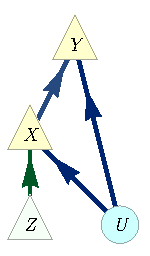
\includegraphics[scale=1]{ISorigDAG.pdf}
    \caption{The instrumental scenario of \citet{pearl1995instrumental}.}
    \label{fig:ISorigDAG}
    \end{minipage}\hfill
    \begin{minipage}[t]{0.3\linewidth}      \centering
    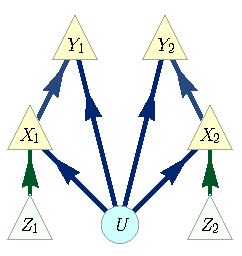
\includegraphics[scale=1]{IScopyDAG.pdf}
    \caption{An inflated DAG of the instrumental scenario which illustrates why coinciding ancestral subgraphs doesn't necessarily imply coinciding marginal distributions.}
    \label{fig:IScopyDAG}
    \end{minipage}\hfill    
    \begin{minipage}[t]{0.3\linewidth}      \centering
    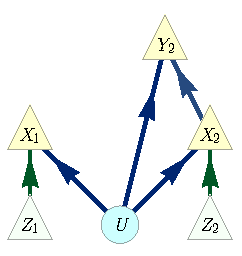
\includegraphics[scale=1]{ISancestorDAG.pdf}
    \caption{The ancestral subgraph of \cref{fig:IScopyDAG} for either $\{X_1 Y_2 Z_1\}$ or $\{X_1 Y_2 Z_2\}$.}
    \label{fig:ancestralsubgraphnotenough}
    \end{minipage}
\end{figure}

In order to avoid any possibility of conclusion, we emphasize that one does not infer constraints on the marginal distributions over $\bm{U}$ and $\bm{V}$ from the mere existence of a copy isomorphism between the subgraphs of $\bm{U}$ and $\bm{V}$ nor from the existence of a copy isomorphism between the ancestral subgraphs of $\bm{U}$ and $\bm{V}$.   Rather, such constraints are inferred from the existence of an inflationary isomorphism between the subgraphs, i.e., the existence of a copy isomorphism between the ancestral subgraphs that restricts to a copy isomorphism between the subgraphs.  
%To be clear, the existence of a copy isomorphism between ancestral subgraphs is \emph{not}, by itself, a sufficient criterion to justify coinciding distributions. Nor is the existence of a copy isomorphism between non-ancestral subgraphs. Rather, the ancestral subgraph isomorphism must reduce to the non-ancestral subgraph isomorphism. 

We emphasize this fact because it might seem, at first glance, that the existence of a copy isomorphism between ancestral subgraphs is {\em by itself} sufficient for deriving constraints on the marginal distributions.  To see why this is not the case, we offer the following example.
%The following example illustrates why the existence of a copy isomorphism between ancestral subgraphs is not, by itself, a sufficient criterion for deriving constraints on the marginal distributions. 
%to justify coinciding distributions.

\begin{comment}
Take as the original DAG the instrumental scenario of \citet{pearl1995instrumental}, and consider the inflation depicted in \cref{fig:IScopyDAG}.  Consider the pair of contexts $\bm{U} = \{ X_1 X_2 Y_1\}$ and $\bm{V}= \{ X_1 X_2 Y_2\}$ on the inflated DAG. 

We will show here that whereas the inflated model satisfies
\begin{align}
P_{X_1 X_2 Y_1} =P_{ X_2 X_1 Y_2},
\end{align}
it does {\em not} satisfy
\begin{align}
P_{X_1 X_2 Y_1} =P_{ X_1 X_2 Y_2}
\end{align}
(where the difference is whether the order of $X_1$ and $X_2$ is the same or different on the two sides of the equation). 

First note that there is a unique copy isomorphism between the subgraphs of $\bm{U}$ and $\bm{V}$, namely,

[NO THIS EXAMPLE DOESN'T WORK!]
\end{comment}



Take as the original DAG the instrumental scenario of \citet{pearl1995instrumental}, and consider the inflation depicted in \cref{fig:IScopyDAG}.  Consider the pair of contexts $\bm{U} = \{ X_1 Y_2 Z_1\}$ and $\bm{V}= \{ X_1 Y_2 Z_2\}$ on the inflated DAG.  Note that these are clearly not pre-injectable sets. 

%Because each context has no two variables that are copy-index equivalent, there is a unique copy isomorphism between them, namely,
The ancestral subgraphs for these two contexts are precisely the same, namely the DAG of~\cref{fig:ancestralsubgraphnotenough}.  This DAG has only the identity map as a graph isomorphism, and therefore this is the unique copy isomorphism between $\ansubgraph{X_1 Y_2 Z_1}$ and $\ansubgraph{X_1 Y_2 Z_2}$.  But if we restrict the domain of this isomorphism to $\subgraph{X_1 Y_2 Z_1}$, we clearly do {\em not} get an isomorphism between $\subgraph{X_1 Y_2 Z_1}$ and $\subgraph{X_1 Y_2 Z_2}$ because $Z_1 \mapsto Z_1$ and we require that $Z_1 \mapsto Z_2$.  (In fact, there are no copy isomorphisms between $\subgraph{X_1 Y_2 Z_1}$ and $\subgraph{X_1 Y_2 Z_2}$ because there are no graph isomorphisms between $\subgraph{X_1 Y_2 Z_1}$ and $\subgraph{X_1 Y_2 Z_2}$.)  %\color{purple} [R: Show the subDAGs in the figure?] \color{black}

%to this copy isomorophism between the ancestral subgraphs does not restrict to a copy isomorphism between the subgraphs. 
%Nevertheless, there is no inflationary isomorphism between ${X_1 Y_2 Z_1}$ and ${X_1 Y_2 Z_2}$, since the non-ancestral subgraphs of these two sets of nodes are not even copy isomorphic, i.e.~$\subgraph{X_1 Y_2 Z_1}\not\sim\subgraph{X_1 Y_2 Z_2}$!

%In general there may exist multiple inflationary isomorphisms, for example the sets $\brackets{A_1 A_2 B_1}$ and $\brackets{A_1 A_2 B_2}$ can be related by either 
%\begin{align}
%    \begin{pmatrix}
%     A_1 \leftrightarrow A_1 \\
%     A_2 \leftrightarrow A_2 \\
%     B_1 \leftrightarrow B_2 \\
%    \end{pmatrix}
%    \qquad\text{or}\qquad
%    \begin{pmatrix}
%     A_1 \leftrightarrow A_2 \\
%     A_2 \leftrightarrow A_1 \\
%     B_1 \leftrightarrow B_2 \\
%    \end{pmatrix}
%\end{align}
% Two inflated DAGs $G'_1$ and $G'_2$ are said to be inflationarily isomorphic if there exists a graph isomorphism between them which is itself also an inflationary isomorphism. This occurs iff $G'_1\sim G'_2$.
% We say that one isomorphim \tblue{contains} another if the rule-set of the latter is a subset of the rule-set of the former.

% If two sets $\bm{X}$ and $\bm{Y}$ are inflationarily isomorphic, then $P(\bm{X}) = P(\bm{Y})$ in any inflated model.

%In other words, $\pdf{\bm{X}}=\pdf{\bm{Y}}$ if and only if an inflationary graph isomorphism exists between $\ansubgraph[G']{\bm{X}}$ and $\ansubgraph[G']{\bm{Y}}$ which preserves the inflationary isomorphism between $\bm{X}$ and $\bm{Y}$. 

One can try to make use of Lemma~\ref{lem:coincide} when deriving polynomial inequalities with inflation via solving the marginal problem, by imposing $P_{\bm{U}} = P_{\bm{\varphi(\bm{U})}}$ as an additional constraint for every inflationary isomorphism $\varphi : \subgraph{\bm{U}}\to\subgraph{\bm{V}}$ between sets of observable nodes. This is advantageous to speed up to the linear quantifier elimination, since one can solve each of the resulting equations for one of the unknown joint probabilities and thereby eliminate that probability directly without Fourier-Motzkin elimination.

Moreover, one could also hope that these additional equations would result in tighter constraints on the marginal problem, which would in turn yielder tighter causal compatibility inequalities. However, our computations have so far not revealed any example of such a tightening. In some cases, this lack of impact can be explained as follows.
% We define two ordered sets of observable nodes $\bm{X}$ and $\bm{Y}$ in some inflated DAG $G'$ to be \tblue{irrelevant to the marginal problem} if there exists a copy bijection $\varphi:\nodes{G'}\to\nodes{G'}$ which satisfies two conditions:
%\begin{enumerate}
%	\item $\varphi$ is a graph isomorphism,
%	\item $\varphi$ maps $\bm{X}$ onto $\bm{Y}$.
%\end{enumerate}
Suppose that $\varphi:\subgraph{\bm{U}}\to\subgraph{\bm{V}}$ is an inflationary isomorphism 
%where the copy isomorphism between the ancestral subgraphs of which it is a restriction is an {\em automorphism} 
which is not just the restriction of a copy isomorphism between the ancestral subgraphs, but even the restriction of a copy automorphism 
$\Phi':G'\to G'$ of the entire inflated DAG onto itself; in particular, this assumption implies that $\Phi'$ also restricts to a copy isomorphism $\Phi:\ansubgraph{\bm{U}}\to\ansubgraph{\bm{V}}$ between the ancestral subgraphs. In this case, the irrelevance of the additional constraint $P_{\bm{U}} = P_{\varphi(\bm{U})}$ to the marginal problem for inflated models can be explained by the following argument. 

Suppose that some joint distribution $P_{\SmallNamedFunction{ObservedNodes}{G'}}$ solves the unconstrained marginal problem, i.e.,~without requiring $P_{\bm{U}} = P_{\varphi(\bm{U})}$. Now apply $\Phi'$ to the variables in $P_{\SmallNamedFunction{ObservedNodes}{G'}}$, switching the variables around, to generate a new distribution $P'=P_{\Phi'(\SmallNamedFunction{ObservedNodes}{G'})}$. Because the set of marginal distributions that arise from inflated models is invariant under this switching of variables, we conclude that $P'$ is also a solution to the unconstrained marginal problem. Taking the uniform mixture of $P$ and $P'$ is therefore still a solution of the unconstrained marginal problem. But this uniform mixture also satisfies the supplementary constraint $P_{\bm{U}} = P_{\varphi(\bm{U})}$. Hence the supplementary constraint is satisfiable automatically whenever the unconstrained marginal problem is solvable, which makes adding the constraint irrelevant.

Note that the argument does not apply if the inflationary isomorphism $\varphi:\bm{U}\to\bm{V}$ cannot be extended to a copy automorphism of the entire inflated DAG. It also does not apply if one uses the $d$-separation conditions beyond ancestral independence  on the inflated DAG as additional constraints, because in this case the set of compatible distributions is not necessarily convex.  In either of these cases, it is not apparent whether or not constraints arising from copy-index equivalence could yield tighter inequalities. 
%We do not know what happens in either of these cases.




\section{Using the Inflation Technqiue to Certify a DAG as ``Interesting"\label{sec:interestingproof}}

By considering all possible $d$-separation conditions implied by a given DAG, one can infer the set of all conditional independence (CI) relations that must hold in any joint distribution over the observed variables that is compatible with the given DAG. In the presence of nontrivial latent nodes, the set of all  \emph{observable} CI relations (that is, CI relations among observed variables) 
%\sout{is a strict subset of the set of all CI relations} 
do not always exhaust the constraints on the joint distribution over the observed variables. \citet{pusey2014gdag} were concerned with identifying DAGs for which an observable distribution satisfying all observable CI relations is \emph{not} a sufficient criterion for compatibility.  They introduced the term \tblue{interesting} to refer to any DAG which exhibits a discrepancy between the set of observable distributions genuinely compatible with it and the set of observable distributions that merely reproduce its observable CI relations.

\citet{pusey2014gdag} derived novel necessary criteria on the structure of a DAG in order for it to be interesting, and they conjectured that their criteria may, in fact, be necessary and sufficient. As evidence in favour of this conjecture, they enumerated all possible DAGs with no more than six nodes satisfying their criteria.
%for further testing. 
They found only 21 unique classes of potentially interesting DAGs.
%after accounting for symmetry \color{purple} [R: I think that the classes contain more than just DAGs that are related by symmetry.] \color{black} 
Of those 21, they further proved that 18 were unambiguously interesting by writing down an explicit incompatible distribution which nevertheless satisfied the DAGs observable CI relations. Incompatibility of the constructed distribution was certified by means of entropic inequalities. 

That left three classes of DAGs  as \emph{potentially} interesting. For each of these, \citet{pusey2014gdag} derived all Shannon-type entropic inequalities in two different ways, once by accounting for non-observable CI relations (that is, CI relations that do not refer exclusively to observed variables) and once without. The existence of \emph{novel} Shannon-type inequalities upon accounting for non-observable CI relations is evidence for the DAG being interesting. The only loophole is that perhaps those novel Shannon-type inequalities are actually non-novel non-Shannon-type inequalities implied by the observable CI relations alone \cite{pusey2014gdag}. %\color{purple} [R: why is this a loophole?] \color{black}

One way to close this loophole would be to show that the novel Shannon-type inequalities imply constraints beyond some inner approximation to the genuine entropy cone absent non-observable CI relations, perhaps along the lines of Ref.~\cite{weilenmann2016entropic}. Another is to use causal compatibility inequalities beyond entropic inequalities to identify some CI-respecting but incompatible distributions. \citet{pianaar2016interesting} accomplished precisely this, and should be credited with the original insight to explicitly consider the different values that an observable root variable might take. In the following, we demonstrate how the inflation technique can be used for this purpose. So far, we have only considered one of the three enigmatic causal structures, namely,~\cref{fig:GDAG15}.

\begin{figure}[b]
\centering
\begin{minipage}[t]{0.4\linewidth}
\centering
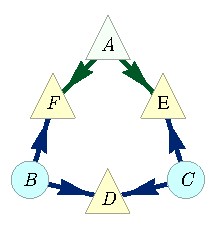
\includegraphics[scale=1]{scen15DAGV2.pdf}
\caption{DAG \#15 in Ref. \cite{pusey2014gdag}.}\label{fig:GDAG15}
\end{minipage}
\hfill
\begin{minipage}[t]{0.5\linewidth}
\centering
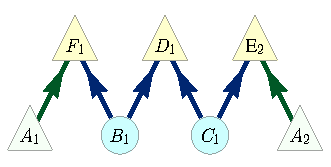
\includegraphics[scale=1]{scen15InflationDAGV2.pdf}
\caption{A useful inflation of \cref{fig:GDAG15}.}\label{fig:Inflated15}
\end{minipage}
\end{figure}

The following representative causal compatibility inequalities for the DAG of~\cref{fig:GDAG15} follow from the inflation technique applied to causal compatibility inequalities for the inflated DAG of \cref{fig:Inflated15}, where the latter are obtained from Hardy-type tautologies as described in \cref{sec:TSEM}:
\begin{align}
\p[A]{0} \p[A D E]{0 0 0} \leq {\p[A E]{0 0} \p[A F]{0 0}  + \p[A]{0} \p[A D F]{0 0 1}}, \\
\p[A]{0}\p[A D E]{1 0 0} \leq {\p[A E]{1 0} \p[A F]{0 0} + \p[A]{1} \p[A D F]{0 0 1}}.
\label{eq:DAG15ineqs}
\end{align}
%\color{purple} [R: Why do we bother to provide the first of these two inequalities given that we do not use it to reject Pienaar's distribution?  Just as something else we can say about this DAG?]\color{black}
For example, the second inequality may be explicitly derived as follows. A Hardy-type tautology on the variables of the inflated DAG implies the following constraint on marginals:
%One Hardy-type probabilistic inequality required for consistency of marginal distributions is
\begin{align}\label{eq:hardyforpienaar}
     \pdf[A_1 A_2 D E_2]{0100} \leq \pdf[A_1 A_2 F_1 E_2]{0100} + \pdf[A_1 A_2 D F_1]{0101} .
\end{align}
Applying factorization as per the ancestral independence relations of the inflated DAG, we obtain 
%the precursor to \cref{eq:DAG15ineqs}, namely
\begin{align}
 \p[A_1]{0} \p[A_2 D E_2]{100} \leq \p[A_1 F_1]{01} \p[A_2 E_2]{00} + \p[A_2]{1} \p[A_1 D F_1]{001},   
\end{align}
and finally translating this into a causal compatibility inequality on the original DAG using \cref{maincorollary}, we obtain \cref{eq:DAG15ineqs}. 
 
%which is equivalent to \cref{eq:DAG15ineqs}.
%A distribution incompatible with \cref{fig:GDAG15} discovered by \citet{pianaar2016interesting} is given by
In \citet{pianaar2016interesting}, it was shown that the following distribution, which is easily verified to satisfy the CI relations among the observed variables of \cref{fig:GDAG15}, namely, $A\indep D$ and $E\indep F | A$~\cite{pusey2014gdag}, is nonetheless incompatible with \cref{fig:GDAG15}:
\begin{align}\label{eq:pienaardistro}
P^{\text{Pien}}_{A D E F}:=\frac{[0000]+[0101]+[1000]+[1110]}{4},\quad\text{i.e.}\quad P^{\text{Pien}}_{A D E F}(a d e f):=\begin{cases}\tfrac{1}{4}&\text{if }  e\eql a\cramp{\cdot} d \text{ and } f\eql  (a\cramp{\oplus} 1)\cramp{\cdot} d , \\ 0&\text{otherwise}.\end{cases}
\end{align}
%which can be easily verified to satisfy the CI relations among the observed variables of the DAG, namely, $A\indep D$ and $E\indep F | A$~\cite{pusey2014gdag}. 

It is easily verified that this distribution violates the causal incompatibility inequality of~\cref{eq:DAG15ineqs}.  It is in this sense that the inflation technique can show that the DAG of \cref{fig:GDAG15} is interesting. 
%demonstrate this incompatibility 
%rules out this distribution because it violates the causal incompatibility inequality~\cref{eq:DAG15ineqs}.

There is another way to see that this distribution is not compatible with~\cref{eq:DAG15ineqs} using the inflation technique.  First, one notes that any marginal distribution on $DEF$ that is compatible with the DAG of \cref{fig:GDAG15} is necessarily also compatible the triangle scenario (where $D$, $E$ and $F$ are the observed variables).
% because making a latent variable observable does not alter serves only to restrict the cardinality of that variable.
Second, one notes that the marginal distribution $P^{\text{Pien}}_{D E F}$ is incompatible with the triangle scenario, since it violates inequality \#8 of~\cref{sec:CCineqs}.  This is the same inequality which rejects the W-distribution of~\cref{eq:wdistribution1}.
Like the W-distribution, the distribution $P^{\text{Pien}}$
 %Yet another interesting point is that $P^{\text{Pien}}$ 
 not only satisfies all Shannon-type entropic inequalities pertinent to~\cref{fig:GDAG15}, but lies within an inner approximation to the genuine entropy cone for that scenario\footnote{This is due to Weilenmann and Colbeck (private correspondence).}. In other words, there exists a distribution with the same joint and marginal entropies as  $P^{\text{Pien}}$ which \emph{is} compatible with \cref{fig:GDAG15}.

Finally, it may be worth noting that the inflation of~\cref{fig:Inflated15} is precisely the ``bilocality scenario'' considered by~\citet{BilocalCorrelations}.  Therefore, the inflation technique permits us to translate every causal compatibility inequality for the bilocality scenario into a causal compatibility inequality for the DAG of~\cref{fig:GDAG15}.

%Interesting, the distribution $P^{\text{Pien}}$ can also be certified incompatible with \cref{fig:GDAG15} using only our results from the Triangle scenario. By marginalizing over the random variable $A$ in \cref{eq:pienaardistro} we obtain tripartite distribution which is rejected by inequality $\#8$ in \cref{tab:machinereadable} and in the table of inequalities on \cpageref{page:nontrivlist}. This is the same inequality which rejects the W-distribution defined in \cref{eq:wdistribution1}.



%\purp{T: I've commented this out since we're not concerned here with observational equivalence, and I have the feeling that it would still require a major clean-up operation. The example of 6 observationally equivalent DAGs is not very good since they are all equivalent to A <-- S --> B, which doesn't contain any latent nodes}
\begin{comment}
\clearpage\section{Recognizing observationally equivalent DAGs}

%\purp{Notes to self: Comment about matching-up latent variables between causal structures, for ObsEquiv test.}

%Without loss of generality we herein consider only deterministic DAGs where all latent variables are parentless. \purp{Either prove this, or remove it. If not invoked we should discuss adding edges TO latent variables.}

One expects that an edge $A\to B$ can be added to DAG $G$ while leaving $G$ observationally invariant if the new connection does not introduce any new information about observable variables to $B$. %If the added connection does inform $B$ about some observable $C$, that's still ok so long as the new informational cannot be exploited to increase the correlation between $B$ and $C$.
We can formalize this notion in the language of sufficient statistics. To do so, however, a few background definitions are in order.

\tblue{Perfectly Predictable:} The random variable $X$ is perfectly predictable from a set of variables $\bm{Z}$, hereafter $\mblue{\bm{Z}\vDash X}$, if $X$ can be completely inferred from knowledge of $\bm{Z}$ alone. In a deterministic DAG, for example, every non-root node is perfectly predictable given its parents, ${\NamedFunction{pa}{\!X\!}\vDash X}$. Indeed, in a deterministic DAG the node $X$ is perfectly predictable from $\bm{Z}$ if $X$ is a deterministic descendant of $\bm{Z}$. Operationally, $X$ is a deterministic descendant of $Z$ if the intersection of {[the ancestors of $X$]} with {[the non-ancestors of $Z$]} is a subset of {[the descendants of $Z$]}. Happily though, perfectly predictability can be extrapolated from a causal structure with minimal effort: ${\bm{Z}\vDash X}$ if every directed path to $X$ from any root node is blocked by $\bm{Z}$. 

\tblue{Markov Blanket:} The Markov Blanket for a set of nodes $\bm{V}$, hereafter $\mblue{\NamedFunction{MB}{\!\bm{V}\!}}$, is the set of all of $\bm{V}$'s children, parents, and co-parents. The Markov Blanket is so defined because the nodes in $\bm{V}$ are conditionally independent of \emph{everything} given $\NamedFunction{MB}{\!\bm{V}\!}$. If the random variables in the Markov Blanket $\NamedFunction{MB}{\!\bm{V}\!}$ are known, then information about nodes inside $\bm{V}$ has no bearing on nodes outside the Markov Blanket and vice versa.

\tblue{Markov Partition:} \purp{New! I made this up Nov 24. Useful do you think?} A set of variables $\bm{Z}$ is a Markov Partition for a pair of random variables $X$ and $Y$, hereafter $\mblue{X\cramp{\dashv}\bm{Z}\cramp{\vdash}Y}$, if the pair are conditionally independent of eachother given \emph{any superset} of $\bm{Z}$. Operationally, this means that $X$ and $Y$ are $d$-separated by every superset of $\bm{Z}$. Equivalently, ${X\cramp{\dashv}\bm{Z}\cramp{\vdash}Y}$ if $\NamedFunction{MB}{\!\bm{V}\!}\subseteq \bm{Z}$ and $X\in \bm{V}$ while $Y\not\in \bm{V}$, or if $\NamedFunction{MB}{\!\bm{V}\!}\subseteq \bm{Z}$ and $Y\in \bm{V}$ while $X\not\in \bm{V}$. Happily though, Markov Partitions can be extrapolated from a causal structure with minimal effort: ${X\cramp{\dashv}\bm{Z}\cramp{\vdash}Y}$ if and only if $X$ and $Y$ would be in \emph{disconnected components} under the deletion of all edges initiation from $\bm{Z}$. 

\tblue{Sufficient Statistic:} A set of nodes $\bm{Z}$ is a sufficient statistic for $A$ relative to $X$, hereafter $\mblue{\bm{Z}\vdash A|X}$,
%$\bm{Z}\in\NamedFunction{SS}{\!A|X\!}$, 
if and only if all inferences about $X$ which can be made given knowledge of $A$ are also inferable \emph{without} knowing $A$ but with knowing $\bm{Z}$ instead. In other words, learning $A$ can never teach anything new about $X$ if $\bm{Z}$ is already known. If $X=A$, then the \emph{only way} $\bm{Z}$ can stand in for $A$ when making inferences about $A$ is if $A$ is perfectly predicable given $\bm{Z}$, i.e. ${\bm{Z}\vdash A|A\iff \bm{Z}\vDash A}$. If $A\neq B$ then there are four \purp{and only four?)} ways that $\bm{Z}\vdash A|X$ can be implied by a DAG: If $\bm{Z}\vDash A$, if $\bm{Z}\vDash X$, if $\NamedFunction{MB}{\!\bm{V}\!}\subseteq \bm{Z}$ and $A\in \bm{V}$ while $X\not\in \bm{V}$, or if $\NamedFunction{MB}{\!\bm{V}\!}\subseteq \bm{Z}$ and $X\in \bm{V}$ while $A\not\in \bm{V}$. \purp{Alternatively:} If $A\neq B$ then there are THREE ways that $\bm{Z}\vdash A|X$ can be implied by a DAG: If $\bm{Z}\vDash A$, if $\bm{Z}\vDash X$, and if ${A\cramp{\dashv}\bm{Z}\cramp{\vdash}X}$.

\begin{theorem}\label{theo:edgeadding}
An edge $A\to B$ can be added to $G$ without observational impact if $\NamedFunction{pa}{\!B\!}$ are a sufficient statistic for $A$ relative to all observable nodes, i.e. $\forall{\text{observable }X}:\NamedFunction{pa}{\!B\!}\vdash A|X$.\\
In particular, the edge $A\to B$ can always be added whenever $\NamedFunction{pa}{\!B\!}\vDash A$, including, but not limited to, the instance  $\NamedFunction{pa}{\!A\!}\subseteq \NamedFunction{pa}{\!B\!}$.\\
Furthermore, the edge $\Lambda\to B$ can be also always be added whenever $\Lambda$ is latent and $\NamedFunction{MB}{\!\Lambda\!}\subseteq\NamedFunction{pa}{\!B\!}$.
\end{theorem}

We can also define an analogous condition for when an edge can be removed from a DAG without impacting it observationally.
\begin{corollary}\label{cor:edgedropping}
An edge $A\to B$ can be dropped from $G$ to form $G'$ such that $G$ and $G'$ are observationally equivalent if \sout{and only if} the edge $A\to B$ can be added (back) to $G'$ while leaving $G'$ observationally invariant per \cref{theo:edgeadding}.
\end{corollary}

On the subject of adding observationally-invariant edges, it is important to recognize when latent nodes can be introduced (or dropped) without observational impact.
\begin{theorem}\label{theo:latentadding}
A (root) latent node $\Lambda$ can be removed from $G$ without observational impact if $\Lambda$ has only one child node and no co-parents ($\Lambda$ is ``equivalent to local randomness"), or if $\Lambda$'s children are also all children of another single latent node ($\Lambda$ is ``covered-for by another latent node"). Conversely, a new root latent node $\Lambda$ can be introduced along with various outgoing edges, without observational impact, if $\Lambda$ would be equivalent to local randomness or covered-for by another latent node.
\end{theorem}

\clearpage
Naturally, two causal structures are observationally equivalent if one can be transformed into the other without observational impact, via \cref{theo:edgeadding,theo:latentadding}. Some examples of observationally equivalent scenarios, and the steps which interconvert them, are given in \cref{fig:equivalences}.
\begin{figure}[hb]
\centering
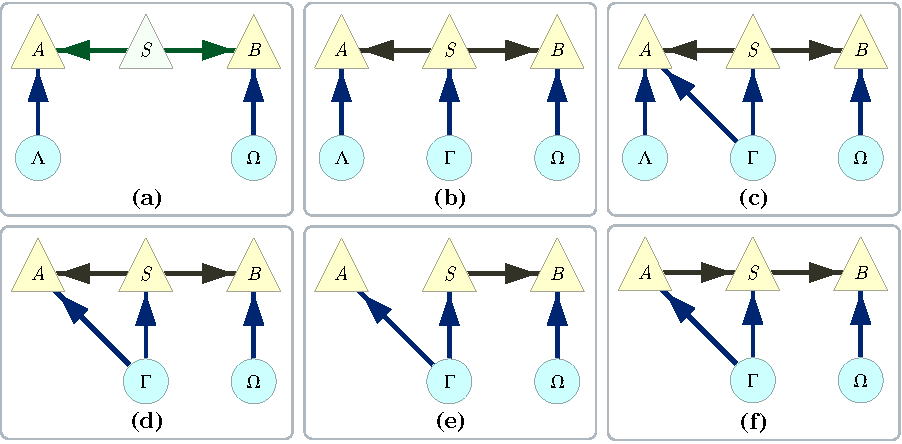
\includegraphics[width=\linewidth]{ObservationalEquivalencesExamples.pdf}
\caption{A set of observational equivalent causal structures. The reasons the changes are observational invariant are as follows: \\
(a)$\sim$(b) because $\Gamma$ is useless in (b), and as such $\Gamma$ can be dropped from (b) per \cref{theo:latentadding}.\\
(b)$\sim$(c) because $\NamedFunction{MB}{\!\Gamma\!}\subseteq\NamedFunction{pa}{\!A\!}$ in (b), and as such $\Gamma\to A$ can be added to (b) per \cref{theo:edgeadding}.\\
(c)$\sim$(d) because $\Lambda$ is redundant to $\Gamma$ in (c), and as such $\Lambda$ can be dropped from (c) per \cref{theo:latentadding}.\\
(d)$\sim$(e) because $\NamedFunction{pa}{\!S\!}\subseteq\NamedFunction{pa}{\!A\!}$ in (e), and as such $S\to A$ can be added to (e) per \cref{theo:edgeadding}.\\
(e)$\sim$(f) because $\NamedFunction{pa}{\!A\!}\subseteq\NamedFunction{pa}{\!S\!}$ in (e), and as such $A\to S$ can be added to (e) per \cref{theo:edgeadding}.
}\label{fig:equivalences}
\end{figure}

%Recall now the two steps of the transformation $\mathsf{ReduceToPCC}$. Imagine after the first step is finished, that an edge $A\to B$ remains, where $A$ is not a root node. Have directly connected all causal pathways, we know that $\NamedFunction{pa}{\!A\!}\subseteq\NamedFunction{pa}{\!B\!}$. As such, $\NamedFunction{pa}{\!B\!}\vDash A$, that is to say, $A$ is perfectly predictable given the parents of $B$. By \cref{theo:edgeadding}, therefore, if the edge $A \to B$ were not in the DAG, we would be able to add that edge without observational impact. By \cref{cor:edgedropping}, therefore, removing that edge has no observational impact. Indeed, the second step of $\mathsf{ReduceToPCC}$ leaves the post-first-step DAG observationally invariant. This allows us to quickly determine if a DAG is PCC-lossless.

%\begin{prop}\label{prop:PCClossless}
%A causal structure $G$ is PCC-lossless if every new edge in $\NamedFunction{ReduceToPCC}{\!G\!}$ relative to $G$ can be accounted for by adding edges to $G$ while leaving $G$ observationally invariant, pursuant to %\cref{theo:edgeadding,theo:latentadding}.
%\end{prop}

%%%%%%%%%%%% Enumeration via lowercase letters
\renewcommand{\labelenumi}{(\alph{enumi})}
\renewcommand{\theenumi}{(\alph{enumi})}
\renewcommand{\labelitemi}{$\circ$}
\end{comment}



\section{The Copy Lemma and Non-Shannon type Entropic Inequalities}\label{sec:NonShannon}

As it turns out, the inflation technique is also useful outside of the problem of causal inference. As we argue in the following, inflation is secretly what underlies the \tblue{Copy Lemma} in the derivation of non-Shannon type entropic inequalities~\cite[Chapter~15]{yeung_network_2008}. The following formulation of the Copy Lemma is the one of \citet{kaced_equivalence_2013}.

\begin{lemma}
	Let $A$, $B$ and $C$ be random variables with distribution $P_{ABC}$. Then there exists a fourth random variable $A'$ and joint distribution $P_{AA'BC}$ such that:
	\begin{enumerate}
		\item $P_{AB} = P_{A'B}$,
		\item $A' \indep AC \:|\: B$.
	\label{copylemma}
	\end{enumerate}
\end{lemma}

The proof via inflation is as follows.
\begin{proof}
We begin by noting that every possible joint distribution $P_{ABC}$ is compatible with a DAG of the form of~\cref{fig:beforecopy}.  This follows from the fact that one may take $X$ to be any \tblue{sufficient statistic} for the joint variable $(A,C)$ given $B$, such as $X := (A,B,C)$.  Next, we consider the inflation of \cref{fig:beforecopy} depicted in~\cref{fig:aftercopy}. The maximal injectable sets are $\{ A_1 B_1 C_1\}$ and $\{A_2 B_1\}$.  By \cref{mainlemma}, because $P_{ABC}$ is assumed to be compatible with~\cref{fig:beforecopy}, it follows that the marginals $\{ P_{A_1 B_1 C_1}, P_{A_2 B_1}\}$, where $P_{A_1 B_1 C_1}:= P_{A B C}$ and $P_{A_2 B_1} := P_{AB}$, are compatible with the inflated DAG of~\cref{fig:aftercopy}.  The fact that $A_2$ is d-separated from $A_1 C_1$ by $B_1$ in ~\cref{fig:aftercopy} implies that the joint distribution can be expressed as $P_{A_1 A_2 B_1 C_1} := P_{A_1 B_1 C_1} \otimes P_{A_2 B_1} \otimes P_{B_1}^{-1}$, which is only defined for those values of $b_1$ such that $P_{B_1}(b_1) \ne 0$.  By construction, $P_{A_1 A_2 B_1 C_1}$ has $P_{A_1 B_1}= P_{A_2 B_1} =P_{AB}$ and satisfies the conditional independence relation $A_2 \indep A_1 C_1 \:|\: B_1$.
%If the original distribution $P_{ABC}$ is compatible with~\cref{fig:beforecopy}, then the associated inflated model marginalizes to a distribution $P_{A_1 A_2 B_1 C_1}$ which has the required properties.
%Consider the original DAG of~\cref{fig:beforecopy} and the associated inflated DAG of~\cref{fig:aftercopy}. If the original distribution $P_{ABC}$ is compatible with~\cref{fig:beforecopy}, then the associated inflated model marginalizes to a distribution $P_{A_1 A_2 B C}$ which has the required properties. To see that every $P_{ABC}$ is compatible with~\cref{fig:beforecopy} one may take $X$ to be any \tblue{sufficient statistic} for the joint variable $(A,C)$ given $B$, such as $X := (A,B,C)$.
\end{proof}


While it is also not hard to write down a distribution with the desired properties explicitly~\cite[Lemma~15.8]{yeung_network_2008}, the fact that one can rederive it using the inflation technique is significant.  For one, all the non-Shannon type inequalities derived by \citet{zeger_2011_nonshannon} are obtained by applying some Shannon type inequality to the distribution that is implied to exist by the Copy Lemma.  Our result shows, therefore, that one can understand these non-Shannon type inequalities for a DAG as arising from Shannon-type inequalities applied to an inflation of the DAG.  Indeed, it may be that the inflation technique may be a more general-purpose tool for deriving non-Shannon-type entropic inequalities.  A natural direction for future research is to explore whether more sophisticated applications of the inflation technique might result  in \emph{new} examples of such inequalities. 
%our purpose in rederiving the lemma via inflation is our hope that more sophisticated applications of the inflation technique will result in \emph{new} non-Shannon type entropic inequalities. 
%For example, all the non-Shannon type inequalities derived by \citet{zeger_2011_nonshannon} are applications of the Copy Lemma, and each proof therein can be recast in terms of some Shannon type inequalities appied to a suitable inflation.

%Note that this inflation is non-broadcasting. The Copy Lemma is therefore valid even in the paradigm of quantum mechanics or any generalized probability theory, as we would expect. \color{purple} [R:Why do we expect this?  Elie's answer: I was thinking that the Copy Lemma should hold regardless of the classical/quantum paradigm, because it is just a way of obtaining non-Shannon type inequalities. The set of jointly-observable variables may differ in classical and quantum theories, but the validity of all Shannon and non-Shannon type inequalities regarding any jointly-observable set is never in question.]\color{black}

\begin{figure}[H]
\centering
\begin{minipage}[t]{0.4\linewidth}
\centering
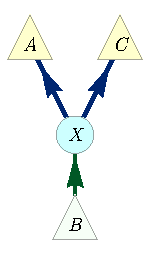
\includegraphics[scale=1]{shannonNOcopyV1.pdf}
\caption{A causal structure that is compatible with any distribution $P_{ABC}$.}\label{fig:beforecopy}
\end{minipage}
\hfill
\begin{minipage}[t]{0.4\linewidth}
\centering
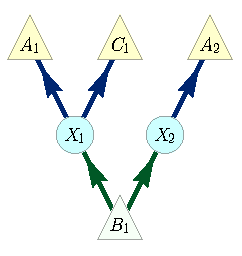
\includegraphics[scale=1]{shannonYEScopyV1.pdf}
\caption{An inflation of \cref{fig:beforecopy}.}\label{fig:aftercopy}
\end{minipage}
%\hfill
%\begin{minipage}[t]{0.3\linewidth}
%\centering
%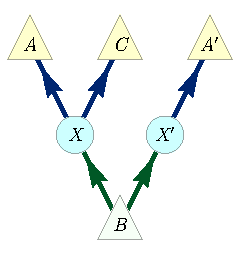
\includegraphics[scale=1]{shannonYEScopyKacedV1.pdf}
%\caption{An equivalent representation of inflation of \cref{fig:aftercopy} so as to match the terminology of \citet{kaced_equivalence_2013}.}
%\end{minipage}
\end{figure}

%\section{Classifying polynomial inequalities for the Triangle scenario}
\section{Causal compatibility inequalities for the Triangle scenario in machine-readable format}
\label{sec:38ineqs}

The following polynomial inequalities for the Triangle scenario with binary observed variables have been derived via the linear quantifier elimination method of~\cref{sec:ineqs} using the inflated DAG of~\cref{fig:Tri222}. Initially this has resulted in 64 symmetry classes of inequalities, where the symmetries are given by permuting the variables and inverting the outcomes. For the resulting 64 inequalities, numerical checks have found violations of only 37 of them: although they are all facets of the marginal polytope over the distributions on pre-injectable sets, there is no guarantee that they are also nontrivial inequalities at the level of the original DAG, and this has indeed turned out not to be the case for 26 of these symmetry classes of inequalities. Moreover, it is still likely to be the case that some of these inequalities are redundant; we have not yet checked whether for every inequality there is a distribution which violates the inequality but satisfies all others.

In the following table, the inequalities are listed in expectation-value form, where we assume the two possible outcomes of each variables to be $\{-1,+1\}$. Each row in the table gives the coefficients with one inequality, which is then $\geq 0$. Inequalities $\#'s (1, 3, 4, 8-17, 19-24)$ in the table are also implied by the hypergraph transversals technique per \cref{sec:TSEM}.

\begin{table*}[ht]\centering\caption{List of inequalities as table of coefficients. This is a machine-readable version of the table in \cref{sec:CCineqs}.\medskip}\label{tab:machinereadable}
\resizebox{\textwidth}{!}{
\begin{tabular}{lc@{\hspace{1em}}ccc@{\hspace{1em}}ccc@{\hspace{1em}}c@{\hspace{1em}}ccc@{\hspace{1em}}ccc@{\hspace{1em}}c} 
%\begin{array}{rrrrrrrrrrrrrrrr}
  & constant & \(\expec{A}\) & \(\expec{B}\) & \(\expec{C}\) & \(\expec{A B}\) & \(\expec{A C}\) & \(\expec{B C}\) & \(\expec{A B C}\) & \(\expec{A}\expec{B}\) & \(\expec{A}\expec{C}\) & \(\expec{B}\expec{C}\) & \(\expec{C}\expec{A B}\) & \(\expec{B}\expec{A C}\) &
   {\(\expec{A}\expec{B C}\)} & {\(\expec{A}\expec{B}\expec{C}\)}   \\\bottomrule
\text{($\#$1):} & 1 & 0 & 0 & 0 & 1 & 1 & 0 & 0 & 0 & 0 & 1 & 0 & 0 & 0 & 0 \\
 \text{($\#$2):} & 2 & 0 & 0 & 0 & 0 & -2 & 0 & 0 & 0 & 0 & 0 & -1 & 0 & 0 & 1 \\
 \text{($\#$3):} & 3 & 1 & -1 & 1 & 1 & 3 & 0 & 0 & 0 & 0 & 1 & -1 & -1 & 0 & 1 \\
 \text{($\#$4):} & 3 & 1 & -1 & 1 & 1 & 3 & 0 & 0 & 0 & 0 & 1 & 1 & -1 & 0 & -1 \\
 \text{($\#$5):} & 3 & 0 & 1 & 0 & 1 & 0 & -2 & 0 & -1 & 1 & 0 & 1 & -1 & 0 & 1 \\
 \text{($\#$6):} & 3 & 0 & 1 & 0 & 0 & -2 & -2 & 0 & 0 & 1 & 0 & -1 & -1 & 0 & 1 \\
 \text{($\#$7):} & 3 & 0 & 1 & 0 & 1 & 0 & -2 & 0 & 1 & -1 & 0 & 1 & 1 & 0 & -1 \\
 \text{($\#$8):} & 3 & 1 & 1 & 1 & 2 & 2 & 2 & -1 & 1 & 1 & 1 & 1 & 1 & 1 & -1 \\
 \text{($\#$9):} & 3 & 1 & 1 & 1 & 0 & 2 & -2 & 1 & -1 & 1 & 1 & 1 & 1 & -1 & -1 \\
 \text{($\#$10):} & 4 & 0 & 0 & 2 & -2 & -2 & 0 & -1 & 2 & 0 & 2 & 1 & 1 & 1 & 0 \\
 \text{($\#$11):} & 4 & 0 & -2 & 0 & -2 & 0 & -3 & 1 & 0 & 0 & 1 & 1 & -1 & 0 & 1 \\
 \text{($\#$12):} & 4 & 0 & -2 & 0 & -2 & -2 & -3 & 1 & 0 & 2 & 1 & 1 & 1 & 0 & -1 \\
 \text{($\#$13):} & 4 & 0 & 0 & 0 & 2 & -2 & 1 & 1 & -2 & -2 & -1 & -1 & 1 & 0 & -1 \\
 \text{($\#$14):} & 4 & 0 & 0 & 0 & 2 & -2 & 1 & 1 & -2 & 2 & -1 & 1 & 1 & 0 & 1 \\
 \text{($\#$15):} & 4 & 0 & 0 & 0 & 0 & -2 & 3 & 1 & 0 & 2 & 1 & -1 & -1 & 0 & 1 \\
 \text{($\#$16):} & 4 & 0 & -2 & 0 & -2 & -2 & -2 & 1 & 0 & 2 & 0 & 1 & 1 & -1 & 0 \\
 \text{($\#$17):} & 4 & 0 & 0 & 0 & -2 & -2 & -2 & 1 & 2 & 2 & 2 & 1 & 1 & 1 & 0 \\
 \text{($\#$18):} & 5 & 1 & 1 & 1 & 3 & 1 & -4 & 0 & -2 & 0 & 1 & 1 & -1 & 0 & 1 \\
 \text{($\#$19):} & 5 & 1 & 1 & 1 & 3 & -1 & -4 & 0 & 2 & -2 & 1 & 1 & 1 & 0 & -1 \\
 \text{($\#$20):} & 5 & 1 & -1 & 1 & 1 & 2 & -2 & -2 & -2 & -1 & 1 & 1 & -2 & -2 & 0 \\
 \text{($\#$21):} & 5 & 1 & 1 & 1 & 1 & 2 & -2 & -1 & 0 & -1 & -1 & 2 & 1 & 1 & -2 \\
 \text{($\#$22):} & 5 & -1 & 1 & 1 & 1 & 1 & -1 & 1 & -2 & -2 & 2 & -2 & -2 & -2 & 0 \\
 \text{($\#$23):} & 5 & 1 & 1 & 1 & 2 & 1 & -1 & 1 & -1 & 0 & 2 & -1 & -2 & -2 & 1 \\
 \text{($\#$24):} & 5 & 1 & 1 & 1 & -1 & 2 & 2 & 1 & -2 & -1 & -1 & 2 & 1 & -1 & -2 \\
 \text{($\#$25):} & 6 & 0 & 0 & 0 & -4 & -3 & 0 & 0 & 2 & 1 & 2 & -2 & -1 & -2 & 1 \\
 \text{($\#$26):} & 6 & -2 & 0 & 2 & -5 & -3 & 0 & 0 & 1 & 1 & 0 & -1 & 1 & -2 & 2 \\
 \text{($\#$27):} & 6 & 0 & 0 & 2 & -4 & 3 & 0 & 0 & 2 & 1 & 0 & -2 & 1 & -2 & 1 \\
 \text{($\#$28):} & 6 & 0 & 0 & 0 & 1 & -3 & 2 & 0 & 1 & 1 & -4 & 1 & -1 & -2 & -2 \\
 \text{($\#$29):} & 6 & 0 & 2 & 0 & 3 & 0 & -5 & 0 & 1 & -2 & 1 & 1 & 2 & 1 & -2 \\
 \text{($\#$30):} & 6 & 0 & 2 & 0 & 2 & -2 & 1 & 0 & -2 & 4 & -1 & 2 & 2 & 1 & 1 \\
 \text{($\#$31):} & 6 & 0 & 0 & 0 & -2 & -3 & -2 & -2 & 0 & 1 & 4 & -2 & -1 & 0 & 1 \\
 \text{($\#$32):} & 7 & 1 & 1 & 1 & 2 & 1 & -3 & 3 & 1 & -2 & 2 & 3 & 2 & -2 & -1 \\
 \text{($\#$33):} & 8 & 0 & 0 & 0 & -2 & -4 & -2 & -3 & 2 & 4 & -2 & -1 & 1 & -3 & 2 \\
 \text{($\#$34):} & 8 & 2 & 0 & -2 & -6 & 1 & 0 & 1 & 0 & -1 & 2 & 1 & 2 & -3 & 3 \\
 \text{($\#$35):} & 8 & 2 & 0 & 0 & 6 & 1 & -2 & 1 & 0 & 1 & 2 & -1 & -2 & -3 & 3 \\
 \text{($\#$36):} & 8 & 0 & -2 & -2 & 0 & -6 & 1 & 1 & 2 & 0 & -1 & 3 & 1 & -2 & -3 \\
 \text{($\#$37):} & 8 & 0 & 2 & 0 & 1 & 2 & -6 & 1 & 1 & -2 & 0 & 2 & 3 & -1 & -3 
\end{tabular}}
\end{table*}


\section{Recovering the Bell inequalities from the inflation technique}
\label{sec:Bellscenarios}


To further illustrate the power of our inflated DAG approach, we now demonstrate how to recover all Bell inequalities~\cite{Brunner2013Bell,bell1966lhvm,CHSHOriginal} via our method. To keep things simple we only discuss the case of a bipartite Bell scenario with two values for both ``settings'' and ``outcome'' variables here, but the case of more parties and/or more values per variable is totally analogous.
%It is critical that our method should be able to derive these seminal criteria, as Bell inequalities have been a foundational component of quantum information theory for the last half century \cite{scarani2012device,BancalDIApproach}.

The causal structure associated to the Bell \cite{bell1964einstein,Brunner2013Bell,bell1966lhvm,CHSHOriginal} experiment [\citealp{pusey2014gdag}~(Fig.~E\#2), \citealp{WoodSpekkens}~(Fig.~19), \citealp{chaves2014novel}~(Fig.~1), \citealp{BeyondBellII}~(Fig.~1), \citealp{wolfe2015nonconvexity}~(Fig.~2b), \citealp{steeg2011relaxation}~(Fig.~2)] is depicted here in \cref{fig:NewBellDAG1}. The observable variables are $A,B,X,Y$, and $\Lambda$ is the latent common cause of $A$ and $B$. In a Bell scenario, one traditionally works with the conditional distribution $P_{AB|XY}$, to be understood as an array of distributions indexed by the possible values of $X$ and $Y$, instead of with the original distribution $P_{ABXY}$, which is what we do.

In the Bell scenario DAG, the maximal pre-injectable sets are
\begin{align}\begin{split}
	\label{eq:bellcontexts}
&\brackets{A_1 B_1 X_1 X_2 Y_1 Y_2} \\
&\brackets{A_1 B_2 X_1 X_2 Y_2 Y_2} \\
&\brackets{A_2 B_1 X_1 X_2 Y_2 Y_2} \\
&\brackets{A_2 B_2 X_1 X_2 Y_2 Y_2} ,
\end{split}\end{align}
where notably every maximal pre-injectable set contains all ``settings'' variables $X_1$ to $Y_2$. The marginal distributions on these pre-injectable sets are then specified by the original observable distribution via
\begin{align}\begin{split}&\forall{a b x_1 x_2 y_1 y_2}:\; \begin{cases}
	P_{A_1 B_1 X_1 X_2 Y_1 Y_2}(a b x_1 x_2 y_1 y_2)  = P_{A B X Y}(a b x_1 y_1) P_X(x_2) P_Y(y_2), \\
	P_{A_1 B_2 X_1 X_2 Y_1 Y_2}(a b x_1 x_2 y_1 y_2)  = P_{A B X Y}(a b x_1 y_2) P_X(x_2) P_Y(y_1), \\
	P_{A_2 B_1 X_1 X_2 Y_1 Y_2}(a b x_1 x_2 y_1 y_2)  = P_{A B X Y}(a b x_2 y_1) P_X(x_1) P_Y(y_2), \\
	P_{A_2 B_2 X_1 X_2 Y_1 Y_2}(a b x_1 x_2 y_1 y_2)  = P_{A B X Y}(a b x_2 y_2) P_X(x_1) P_Y(y_1), \\
\hspace{2.5pc}	P_{X_1 X_2 Y_1 Y_2}(x_1 x_2 y_1 y_2)  = P_X(x_1) P_X(x_2) P_Y(y_1) P_Y(y_2).
\end{cases}\end{split}\end{align}
%where it should be understood implicitly that the inequalities hold for all values of $\{a b x_1 x_2 y_1 y_2\}$.
%The last equations follows from each of the others by making use of the Markov condition $P_{XY} = P_X P_Y$ for the original distribution, it nevertheless
By dividing each of the first four equations by the fifth, we obtain
\begin{align}\begin{split}
	\label{eq:bellfactor}
	\forall{a b x_1 x_2 y_1 y_2}:\; \begin{cases}
	P_{A_1 B_1 | X_1 X_2 Y_1 Y_2}(a b | x_1 x_2 y_1 y_2)  = P_{A B | X Y}(a b | x_1 y_1), \\
	P_{A_1 B_2 | X_1 X_2 Y_1 Y_2}(a b | x_1 x_2 y_1 y_2)  = P_{A B | X Y}(a b | x_1 y_2), \\
	P_{A_2 B_1 | X_1 X_2 Y_1 Y_2}(a b | x_1 x_2 y_1 y_2)  = P_{A B | X Y}(a b | x_2 y_1), \\
	P_{A_2 B_2 | X_1 X_2 Y_1 Y_2}(a b | x_1 x_2 y_1 y_2)  = P_{A B | X Y}(a b | x_2 y_2).
\end{cases}\end{split}\end{align}
The existence of a joint distribution over all six variables---i.e.~the existence of a solution to the marginal problem---implies in particular
%If we then impose marginal compatibility according the the marginal problem we find that the (minimal!) consequence of the inflation hypothesis is 
\begin{align}
	\forall{a b x_1 x_2 y_1 y_2}: \quad P_{A_1 B_1 | X_1 X_2 Y_1 Y_2}(a b | x_1 x_2 y_1 y_2)  =  \sum\nolimits_{a',b'} P_{A_1 A_2 B_1 B_2 X_1 X_2 Y_1 Y_2}(a a' b b'|x_1 x_2 y_1 y_2),
\end{align}
and similarly for the other three conditional distributions under consideration. For consistency with the causal hypothesis, therefore, the original distribution must satisfy in particular
\begin{align}\begin{split}\label{eq:finalBellstep}\forall{a b}:\; \begin{cases}
	P_{A B | X Y}(a b | 0 0)  =  \sum\nolimits_{a',b'} P_{A_1 A_2 B_1 B_2 X_1 X_2 Y_1 Y_2}(a a' b b'|0101) \\
	P_{A B | X Y}(a b | 1 0)  =  \sum\nolimits_{a',b'} P_{A_1 A_2 B_1 B_2 X_1 X_2 Y_1 Y_2}(a' a b b'|0101) \\
	P_{A B | X Y}(a b | 0 1)  =  \sum\nolimits_{a',b'} P_{A_1 A_2 B_1 B_2 X_1 X_2 Y_1 Y_2}(a a' b' b|0101) \\
	P_{A B | X Y}(a b | 1 1)  =  \sum\nolimits_{a',b'} P_{A_1 A_2 B_1 B_2 X_1 X_2 Y_1 Y_2}(a' a b' b|0101)
\end{cases}\end{split}\end{align}
The possibility to write the conditional probabilities in the Bell scenario in this form is equivalent to the existence of a latent variable model, as noted in Fine's Theorem~\cite{FineTheorem}. Thus, if an inflated model exists with the required marginals, then a latent variable model of the original distribution exists as well (and conversely, trivially). Hence the inflated DAG of~\cref{fig:BellDagCopy1} provides necessary and sufficient conditions for the consistency of the original observed distribution with the Bell scenario causal structure.

%The last equations turns out to be rather useful to write down explicitly: putting $x_1 = y_1 = 0$ and $x_2 = y_2 = 1$ and dividing the first equation by the last one results in
%\begin{align*}
%	P_{A B X Y}(a b | 0 0)  =  \sum_{a',b'} P_{A_1 A_2 B_1 B_2 X_1 X_2 Y_1 Y_2}(aa'bb'|0101).
%\end{align*}
%Similarly, $P_{A B X Y}(a b | 0 1)$, $P_{A B X Y}(a b | 1 0)$ and $P_{A B X Y}(a b | 1 1)$ can also be written as marginals of a conditional distribution. 
%By Fine's Theorem~\cite{FineTheorem}, this implies the existence of a hidden-variable model. Conversely, if a hidden-variable model exists, then the existence of the inflated model implies the existence of a solution to the marginal problem.

% In conclusion, we therefore find in the case of the inflated DAG~\cref{fig:BellDagCopy1}, the inflation method yields necessary and sufficient infeasibility criteria for the Bell causal structure, i.e. the Bell/CHSH inequalities, just by requiring marginal compatibility of the pre-injectable sets.
% More generally, we can use Fine's theorem to show that applying the marginal problem to suitable inflated DAGs can reproduce \emph{all} Bell inequalities, for any standard Bell scenario, no matter how many parties or settings or possible outcomes. 

Moreover, it is possible to describe the marginal polytope over the pre-injectable sets of~\cref{eq:bellcontexts}, due to the fact that the ``settings'' variables $X_1$ to $Y_4$ occur in all four contexts. This description is easier to state for the marginal \emph{cone}, by which we mean the convex cone spanned by the marginal polytope, i.e.~the convex cone consisting of all nonnegative linear combinations of deterministic assignments of values, or equivalently the convex cone of all measures on the set of joint outcomes. This cone lives in $\oplus_{i=1}^4 \mathbb{R}^{2^6} = \oplus_{i=1}^4 (\mathbb{R}^2)^{\otimes 6}$, where each tensor factor has basis vectors corresponding to the two possible outcomes of each variable, and the direct summands enumerate the four contexts. Now the marginal cone is precisely the set of all nonnegative linear combinations of the points
\begin{align*}
	(e_{A_1} & \otimes e_{B_1} \otimes e_{X_1} \otimes e_{X_2} \otimes e_{Y_1} \otimes e_{Y_2}) \\
	\oplus\: (e_{A_1} & \otimes e_{B_2} \otimes e_{X_1} \otimes e_{X_2} \otimes e_{Y_1} \otimes e_{Y_2}) \\
	\oplus\: (e_{A_2} & \otimes e_{B_1} \otimes e_{X_1} \otimes e_{X_2} \otimes e_{Y_1} \otimes e_{Y_2}) \\
	\oplus\: (e_{A_2} & \otimes e_{B_2} \otimes e_{X_1} \otimes e_{X_2} \otimes e_{Y_1} \otimes e_{Y_2}),
\end{align*}
where all six variables range over their deterministic outcomes. Since the last four tensor factors occur in every direct summand in exactly the same way, the resulting marginal cone is linearly isomorphic to the cone generated by all vectors of the form
\[
	\left[ (e_{A_1} \otimes e_{B_1}) \oplus (e_{A_1} \otimes e_{B_2}) \oplus (e_{A_2} \otimes e_{B_1}) \oplus (e_{A_2} \otimes e_{B_2})\right] \otimes \left[ e_{X_1} \otimes e_{X_2} \otimes e_{Y_1} \otimes e_{Y_2}\right]
\]
in $\mathbb{R}^{2^2}\otimes \mathbb{R}^{2^4}$. Now since the first four variables in the first tensor factor vary completely independently of the latter four variables in the second tensor factor, the resulting cone will be precisely the tensor product~\cite{namioka_tensor_1969} of two cones: first, the cone generated by all vectors of the form
\[
	(e_{A_1} \otimes e_{B_1}) \oplus (e_{A_1} \otimes e_{B_2}) \oplus (e_{A_2} \otimes e_{B_1}) \oplus (e_{A_2} \otimes e_{B_2}),
\]
and second the one spanned by all $e_{X_1} \otimes e_{X_2} \otimes e_{Y_1} \otimes e_{Y_2}$. While the latter cone is simply the standard positive cone of $\mathbb{R}^8$, the former cone is the cone generated by the ``local polytope'' or ``Bell polytope'' that is traditionally used in the context of Bell scenarios~\cite[Sec.~II.B]{Brunner2013Bell}. Standard results on tensor products of cones and polytopes~\cite{bogart_hom_2013} therefore imply that our marginal polytope is the tensor product of the Bell polytope, corresponding to the $A_1$ to $B_2$ part, with a simplex corresponding to the $X_1$ to $Y_2$ ``settings'' part. This implies that the facets of our marginal polytope are precisely the pairs consisting of a facet of the Bell polytope and a facet of the simplex. For example, in this way we obtain one version of the CHSH inequality as a facet of the marginal polytope,
\[
	\sum_{a,b,x,y} (-1)^{a + b + xy} P_{A_x B_y X_1 X_2 Y_1 Y_2}(a b 0 1 0 1) \leq 2 P_{X_1 X_2 Y_1 Y_2}(0101).
\]
Upon using~\cref{eq:bellfactor}, this becomes
\begin{align*}
	\sum_{a,b} (-1)^{a + b} \big( & P_{A B X Y}(ab00)P_X(1)P_Y(1) + P_{A B X Y}(ab01)P_X(1)P_Y(0) \\
	& + P_{A B X Y}(ab10)P_X(0)P_Y(1) - P_{A B X Y}(ab11)P_X(0)P_Y(0) \big) \leq P_X(0)P_X(1)P_Y(0)P_Y(1),
\end{align*}
so that dividing by the right-hand side results in essentially the conventional form of the CHSH inequality,
\[
	\sum_{a,b} (-1)^{a + b} \left( P_{AB|XY}(ab|00) + P_{AB|XY}(ab|01) + P_{AB|XY}(ab|10) - P_{AB|XY}(ab|11) \right) \leq 2.
\]
In conclusion, the inflation technique is powerful enough to get a precise characterization of all distributions consistent with the Bell causal structure, and our technique for generating polynomial inequalities while solving the marginal problem recovers all Bell inequalities.

It is worth noting that the Bell inequalities may also be derived using the hypergraph-transversals / logical-tautologies technique discussed in \cref{sec:TSEM}. For example, the inequality
\begin{align}\label{eq:preBell}\begin{split}
& \p[A_1 B_1 X_1 Y_1]{1111}\p[X_2]{0} \p[Y_2]{0} \\
&\leq
 \p[A_1 B_2 X_1 Y_2]{1010}\p[X_2]{0} \p[Y_1]{1} +\p[A_2 B_1 X_2 Y_1]{0101}\p[X_1]{1}\p[Y_2]{0}+  \p[A_2 B_2 X_2 Y_2]{1100}\p[X_1]{1} \p[Y_1]{1}
\end{split}\end{align}
is a clear precursor of the Bell inequality
\begin{align}\label{eq:aBell}
 \p[A B | X Y]{11|11} &\leq \p[A B | X Y]{10|10} +\p[A B | X Y]{01|01}+  \p[A B | X Y]{11|00}
\end{align}
as \cref{eq:aBell} is obtained from \cref{eq:preBell} by dividing both sides by $\p[X_1 Y_1 X_2 Y_2]{1100}=\p[X_1]{1} \p[Y_2]{1}\p[X_2]{0} \p[Y_2]{0}$ and then dropping copy indices. On the other hand, \cref{eq:preBell} follows directly from factorization of preinjectable sets and the tautology
\begin{align}\begin{split}
&[ \mgreen{A_1 \eql 1}, \mgreen{B_1 \eql 1}, \mgreen{X_1 \eql 1}, \mgreen{Y_1\eql 1}, \mgreen{X_2 \eql 0}, \mgreen{Y_2 \eql 0}]\\
 & \implies 
 [ \mgreen{A_1 \eql 1}, B_2 \eql 0, \mgreen{X_1 \eql 1}, \mgreen{Y_1\eql 1}, \mgreen{X_2 \eql 0}, \mgreen{Y_2 \eql 0}]
\lor [ A_2 \eql 0, \mgreen{B_1 \eql 1}, \mgreen{X_1 \eql 1}, \mgreen{Y_1\eql 1}, \mgreen{X_2 \eql 0}, \mgreen{Y_2 \eql 0}] \\&\lor [ A_2 \eql 1, B_2 \eql 1, \mgreen{X_1 \eql 1}, \mgreen{Y_1\eql 1}, \mgreen{X_2 \eql 0}, \mgreen{Y_2 \eql 0}].
\end{split}\end{align}

\begin{comment}


\color{purple} Worth noting that possibilistic marginal problem is sufficient to get the Bell inequalities?  If so, here's the beginning of the story. 

The tautology that we have used can be expressed as
\begin{align}
&[ X_1 \eql 0 \land X_2\eql 1 \land Y_1 \eql 0 \land Y_2 \eql 1]\\
& \implies 
 [ X_1 \eql 0 \land Y_1 \eql 0 \land A_1\ne B_1] \lor  [ X_1 \eql 0 \land Y_2 \eql 1 \land A_1\ne B_2]\\
&\lor [ X_2 \eql 1 \land Y_1 \eql 0 \land A_2\ne B_1] \lor [ X_2 \eql 1 \land Y_2 \eql 1 \land A_2 \eql  B_2].
\end{align}
which implies, by the union bound that
\begin{align}
%P_{X_1 X_2Y_1  Y_2}(0101) \le \sum_{x} P_{ X_1 Y_1 A_1 B_1] }(00 x\bar{x} ) + \sum_{ x} P_{ X_1 Y_2 A_1 B_2] }(01 x\bar{x} ) + \sum_{ x} P_{ X_2 Y_1 A_2 B_1] }(01 x\bar{x} ) + \sum_{x} P_{ X_2 Y_2 A_1 B_2 }(01 xx ).
 \p{a_1 b_1 x_1 y_1}\p{\n{x}_2} \p{\n{y}_2}
&\leq
 \p{a_1 \n{b}_2 x_1 \n{y}_2}\p{\n{x}_2} \p{y_1} +\p{\n{a}_2 b_1 \n{x}_2 y_1}\p{x_1}\p{\n{y}_2}+  \p{a_2 b_2 \n{x}_2 \n{y}_2}\p{x_1} \p{y_1}
\end{align}



Using the ancestral independence of $X_1$, $X_2$, $Y_1$, and $Y_2$, we infer that $P_{X_1 X_2Y_1  Y_2} = P_{X_1} P_{ X_2} P_{Y_1} P_{Y_2}$.  

Dividing through by $P_{X_1} P_{ X_2} P_{Y_1} P_{Y_2}$, we get...

\color{black}
\end{comment}
\begin{comment}
Analysis of the inflated DAG in \cref{fig:BellDagCopy1} shows that  
\begin{align}\label{eq:bellypolymapped}
 \p{a b x y}\p{\n{x}} \p{\n{y}}
&\leq
 \p{a \n{b} x \n{y}}\p{\n{x}}\p{y} +  \p{\n{a} b \n{x} y}\p{x} \p{\n{y}}+\p{a b \n{x} \n{y}}\p{x} \p{y}
\\
\shortintertext{by virtue of the unmapped (but factored) inequality}
\label{eq:bellypolyunmapped}
 \p{a_1 b_1 x_1 y_1}\p{\n{x}_2} \p{\n{y}_2}
&\leq
 \p{a_1 \n{b}_2 x_1 \n{y}_2}\p{\n{x}_2} \p{y_1} +\p{\n{a}_2 b_1 \n{x}_2 y_1}\p{x_1}\p{\n{y}_2}+  \p{a_2 b_2 \n{x}_2 \n{y}_2}\p{x_1} \p{y_1}
\end{align}
where \emph{every} probability appearing in \cref{eq:bellypolyunmapped} maps to the original scenario, hence yielding \cref{eq:bellypolymapped}. To derive the usual Bell inequalities from \cref{eq:bellypolymapped} we switch to conditional probabilities via ${\p{a b x y}\to\p{a b | x y}\p{x y}=\p{a b | x y}\p{x}\p{y}}$ which, after dividing both sides of \cref{eq:bellypolymapped} by $\p{x}\p{\n{x}}\p{y}\p{\n{y}}$, yields
\begin{align}\label{eq:chwithneg}
&\p{a b | x y}
\leq
{\p{a \n{b} | x \n{y}} + \p{\n{a} b | \n{x} y}+\p{a b | \n{x} \n{y}}}
\\
\hspace{-\mathindent}\text{or, equivalently,}\quad
\label{eq:chwithoutneg}
&{\p{a b | x y}+\p{a b | x \n{y}} + \p{a b | \n{x} y}}
\leq
{\p{a|\n{x}}+\p{b|\n{y}} + \p{a b | \n{x} \n{y}}}
\end{align}
which is precisely the Clauser-Horne (CH) inequality \cite{CHInequality} for the Bell scenario. Note that to obtain \cref{eq:chwithoutneg} from \cref{eq:chwithneg} we implicitly made use of the no-signalling assumptions, namely $\p{a|x y}=\p{a|x}$ and $\p{b| x y}=\p{b | y}$. The CH inequality is the \emph{unique} Bell inequality (up to permutations) for the Bell scenario if $\brackets{A,B,X,Y}$ are all binary, and hence the CH inequality is a necessary and sufficient criterion to ascertain if correlations are compatible with that Bell scenario variant.

The causal structure of a Bell scenario can also be formulated directly in terms of conditional random variables. For example, the conditional-structure interpretation of \cref{fig:BellDagCopy1} is \cref{fig:BellConditionalDAG}. 

\begin{figure}[t]
\centering
\begin{minipage}[t]{0.45\linewidth}
\centering
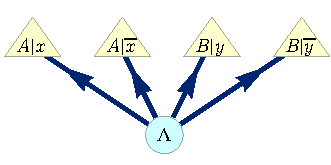
\includegraphics[scale=1]{BellDagConditionForm.pdf}
\caption{The causal structure of the Bell scenario expressed in a form which makes use of conditional random variables.}\label{fig:BellConditionalDAG}
\end{minipage}
%\hfill
%\begin{minipage}[t]{0.45\linewidth}
%\centering
%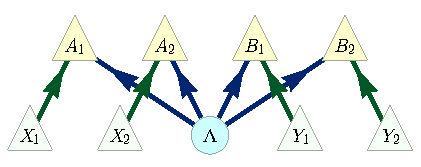
\includegraphics[scale=1]{BellDagCopy.pdf}
%\caption{An inflated DAG of the Bell scenario, where both local settings variables have been duplicated.}\label{fig:BellDagCopy}
%\end{minipage}
\end{figure}

The Bell inequalities are then self-evident from \cref{fig:BellConditionalDAG} without the need for an inflated DAG. The conditional-structure formulation innately implies its own inaccessible gedankenprobabilities, such as $\{\p{a|x , a|\n{x}}$, $\p{a|x , \n{a}|\n{x}},...\}$ etc. By eliminating these gedankenprobabilities from the set of inequalities generated by $0\leq \pdf{A|x , A|\n{x} , B|y , B|\n{y}}$ we obtain
\begin{align}\label{eq:bellcondeq}
0
\leq
{\p{a|\n{x}} + \p{b|\n{y}} + \p{a|x , b|y} -\p{a|x ,b|\n{y}} -\p{a|\n{x} , b|y} -\p{a|\n{x} , b|\n{y}}}\,,
\end{align}
for example. It should be clear that \cref{eq:bellcondeq} is equivalent to \cref{eq:chwithoutneg}.
\end{comment}

%We can perform quantifier elimination on the set of (polynomial) inequalities given by $0\leq \pdf{A|x , A|\n{x} , B|y , B|\n{y}}$. The use of a conditional-structure DAG innately implies certain inaccessible gedankenprobabilities, such as $\{\p{a|x , a|\n{x}}$, $\p{a|x , \n{a}|\n{x}},...\}$ etc. 
%\purp{Rob says kill next two paragraphs?}

%Conditional-structure gedankenprobabilities are somewhat different from the inflated DAG kind, in that they reference multiple counterfactual events, such as ``What is the probability that Alice would choose to visit the museum \emph{IF} (given that) it's a rainy day in Maryland \emph{AND} that Alice would choose to go the beach \emph{IF} (given that) it's sunny in Maryland?". By contrast, unconditional gedankenprobabilities which live on an inflated DAG reference multiple heterofactual (for lack of a better word) events, such as ``What is the probability that Alice-copy-\#1 chooses to visit the museum \emph{AND} that it's raining in Maryland-copy-\#1 \emph{AND} that Alice-copy-\#2 chooses to go the beach \emph{AND} that it's sunny in Maryland-copy-\#2?". 

%Joint counterfactual probabilities are experimentally inaccessible, just the same as joint heterofactual probabilities are. Suppose one could establish both Alice's propensity for going to the museum when it rains and her propensity for going to the beach when it's sunny. Even so, neither the joint counterfactual probability nor the joint heterofactual probability can be established from that limited data. For example, the value of the hidden variable ${\Lambda\cramp{=}\lambda}$ may influence Alice's willingness to get out of bed at all, or determine if she is on-call as a volunteer EMT on a particular day, or $\lambda$ might encode if Alice is travelling out-of-state. If we could measure $\p{a|x , \n{a}|\n{x}},...\}$ we might learn that Alice's likelihood of visiting the museum if it rains in Maryland is highly correlated with her likelihood of visiting the beach when it's sunny in Maryland. Or we might learn that those two counterfactual probabilities are relatively statistically independent. The ``hidden-ness" of the classical variable corresponding to the latent node shields the gedankenprobabilities from being determined. 




%\section*{References}
%\nocite{*}
%\setlength{\bibsep}{\smallskipamount}
%\clearpage
\renewcommand\section{\stdsection}
\let\cleardoublepage\clearpage
\setlength{\bibsep}{3pt plus 3pt minus 2pt}
\bibliographystyle{apsrev4-1}
\nocite{apsrev41Control}
\bibliography{hardyinference}
\end{document}
